% !TeX encoding = UTF-8
% !TeX program = xelatex
% !TeX spellcheck = en_US

\documentclass[
    degree=master, 
    degree-type=professional,
    language=chinese,
    fontset=windows
]{ustcthesis}
% \documentclass[degree-type=professional]{ustcthesis}
% \documentclass[language=chinese]{ustcthesis}
% \documentclass[fontset=windows]{ustcthesis}
% degree      = doctor | master | bachelor
% degree-type = academic | professional
% language    = chinese | english
% fontset     = windows | mac | ubuntu | fandol

% 加载宏包、全部的配置
% !TeX root = ./main.tex

\ustcsetup{
  title              = {容器化CI/CD流水线调度系统设计与实现},
  title*             = {Design and Implementation of a Containerized CI/CD Pipeline Scheduling System},
  author             = {冯嘉泰},
  author*            = {Feng Jiatai},
  speciality         = {软件工程},
  speciality*        = {Software Engineering},
  supervisor         = {李曦~教授, 张文平~高级工程师},
  supervisor*        = {Prof. Li Xi, SE. Zhang Wenping},
  date               = {2024-03-09},  % 默认为今日
  % professional-type  = {专业学位类型},
  % professional-type* = {Professional degree type},
  % department         = {数学科学学院},  % 院系,本科生需要填写
  % student-id         = {PB11001000},  % 学号,本科生需要填写
  % secret-level       = {秘密},     % 绝密|机密|秘密|控阅,注释本行则公开
  % secret-level*      = {Secret},  % Top secret | Highly secret | Secret
  % secret-year        = {10},      % 保密/控阅期限
  % reviewer           = true,      % 声明页显示“评审专家签名”
  %
  % 数学字体
  % math-style         = GB,  % 可选:GB, TeX, ISO
  math-font          = xits,  % 可选:stix, xits, libertinus
}


% 加载宏包

% 定理类环境宏包
\usepackage{amsthm}

% 插图
\usepackage{graphicx}

% 三线表
\usepackage{booktabs}

% 跨页表格
\usepackage{longtable}

% 算法
\usepackage[ruled,linesnumbered]{algorithm2e}

% SI 量和单位
\usepackage{siunitx}

% 参考文献使用 BibTeX + natbib 宏包
% 顺序编码制
\usepackage[sort]{natbib}
\bibliographystyle{ustcthesis-numerical}

% 著者-出版年制
% \usepackage{natbib}
% \bibliographystyle{ustcthesis-authoryear}

% 本科生参考文献的著录格式
% \usepackage[sort]{natbib}
% \bibliographystyle{ustcthesis-bachelor}

% 参考文献使用 BibLaTeX 宏包
% \usepackage[style=ustcthesis-numeric]{biblatex}
% \usepackage[bibstyle=ustcthesis-numeric,citestyle=ustcthesis-inline]{biblatex}
% \usepackage[style=ustcthesis-authoryear]{biblatex}
% \usepackage[style=ustcthesis-bachelor]{biblatex}
% 声明 BibLaTeX 的数据库
% \addbibresource{bib/ustc.bib}

% 配置图片的默认目录
\graphicspath{{figures/}}

% 数学命令
\makeatletter
\newcommand\dif{%  % 微分符号
  \mathop{}\!%
  \ifustc@math@style@TeX
    d%
  \else
    \mathrm{d}%
  \fi
}
\makeatother
\newcommand\eu{{\symup{e}}}
\newcommand\iu{{\symup{i}}}

% 用于写文档的命令
\DeclareRobustCommand\cs[1]{\texttt{\char`\\#1}}
\DeclareRobustCommand\env[1]{\texttt{#1}}
\DeclareRobustCommand\pkg[1]{\textsf{#1}}
\DeclareRobustCommand\file[1]{\nolinkurl{#1}}

% hyperref 宏包在最后调用
\usepackage{hyperref}



\begin{document}

\maketitle
\copyrightpage

\frontmatter
% !TeX root = ../main.tex

\ustcsetup{
  keywords  = {持续集成, 持续交付, 研发效能, 敏捷开发, 任务调度},
  keywords* = {Continue Integration, Continuous Delivery, Development Efficiency, Agile Development, Task Scheduling},
}

\begin{abstract}
  摘要分中文和英文两种,中文在前,英文在后,博士论文中文摘要一般 800~1500 个汉字,硕士论文中文摘要一般 500~1000 个汉字。
  英文摘要的篇幅参照中文摘要。

  关键词另起一行并隔行排列于摘要下方,左顶格,中文关键词间空一字或用分号“,”隔开,英文关键词之间用逗号“,”或分号“;”隔开。

  中文摘要是论文内容的总结概括,应简要说明论文的研究目的、基本研究内容、研究方法或过程、结果和结论,突出论文的创新之处。
  摘要应具有独立性和自明性,即不用阅读全文,就能获得论文必要的信息。
  摘要中不宜使用公式、图表,不引用文献。

  中文关键词是为了文献标引工作从论文中选取出来用以表示全文主题内容信息的单词和术语,一般 3~8 个词,要求能够准确概括论文的核心内容。
\end{abstract}

\begin{abstract*}
  This is a sample document of USTC thesis \LaTeX{} template for bachelor,
  master and doctor. The template is created by zepinglee and seisman, which
  orignate from the template created by ywg. The template meets the
  equirements of USTC thesis writing standards.

  This document will show the usage of basic commands provided by \LaTeX{} and
  some features provided by the template. For more information, please refer to
  the template document ustcthesis.pdf.
\end{abstract*}

\tableofcontents
\listoffigures
\listoftables
% \input{chapters/notation.tex}

\mainmatter
% !TeX root = ../main.tex

\chapter{绪论}

\section{系统开发背景和意义}
随着软件行业的快速发展,软件产品逐渐产生了需求变更频繁、产品迭代加快的趋势,这对软件的开发模式提出了新的挑战。
在过去,传统的软件开发团队普遍遵循瀑布模型,这一模型强调阶段划分,各个阶段必须严格按照时间先后进行,而且每个阶段都必须有产出物才能开始下个阶段\cite{瀑布模型}。
但是由于瀑布模型需要详尽的文档,这就要求在软件开发之初就对用户需求有着全面的了解,这在当下需求频繁变更的互联网时代几乎不可能;
同时,由于瀑布模型的集成式、阶段式的特点,产品的更迭速度势必缓慢,这也不符合现代的快速产品更迭的需求。
所以在当下,瀑布模型已经不符合大部分企业的要求,于是敏捷开发、DevOps、持续集成、持续交付等概念应运而生。

敏捷开发模型强调一组开发流程的反复迭代,要求开发人员采用XP、SCRUM等方法,通过紧密协作实现快速开发和交付。
敏捷开发鼓励以开发人员之间的频繁交流取代严格的文档,同时强调快速发布出软件的初代原型,以满足用户的基本需求,其余的功能和优化点将在后续的反复迭代中逐步完善\cite{敏捷开发}。
敏捷开发比瀑布模型更为灵活,但同时在开发人员和运维人员之间产生了矛盾:
开发人员追求快速迭代交付,而频繁的版本交付势必会加剧软件风险,与运维人员追求系统稳定形成了矛盾。

在开发与运维人员矛盾不断增加的背景下,DevOps(Development和Operations)理念产生并开始成为主流。
DevOps理念强调开发与运维的联合,旨在促进开发和运维过程中信息的流通,打破不同团队间的隔阂,以应对软件的快速变化\cite{DevOps}。
它要求运维人员不应等到软件交付后再进行运维,而是参与进软件的开发初期阶段,与开发人员的迭代周期进行同步的集成与交付。
但是,高频的测试、部署与交付显然不能依赖人力进行操作,这就要求DevOps拥有一套能够持续集成和持续交付的自动化工具。

持续集成(Continuous Integration,CI)和持续交付(Continuous Delivery,CD)是DevOps理念中重要的方法论。
持续集成是软件开发的迭代过程,团队成员不断上传代码至代码仓库,进行集成和测试,实现软件的快速迭代\cite{绪论持续集成1}。
这种方法不仅实现了DevOps的理念,及早发现问题和在早期交付可用原型,还通过强化开发团队与运维团队的联系,降低了团队成员的人工任务。
团队成员在持续集成中频繁集成工作成果,每日至少一次,通过自动构建的检验迅速发现集成错误。
与此同时,持续交付的核心思想是通过创建可重复、可靠的操作过程(一般称为流水线),将软件从概念变为现实\cite{绪论持续集成2}。
持续交付流水线将软件交付过程分成多个阶段,每个阶段验证新特性的质量,确认新功能,防止潜在错误对用户造成不良影响。
持续集成与持续交付继承了DevOps开发理念,成为现代软件工程中的必要环节,这种综合应用不仅简化了开发流程,也提高了软件开发的效率和质量。

当前,各个企业内均普遍使用持续集成与持续交付流水线(下文称“CI/CD流水线”)服务来完成内部的系统集成与交付\cite{1013369056.nh}。
市面上以Jenkins为代表的CI/CD流水线服务可以满足企业的基本开发需求,但随着企业业务的拓展与系统数量的增加,已经越来越难以满足不同团队的个性化需求。

结合以上背景,设计并且研发一套能够满足不同类型开发团队需求,且能保证高易用性、高稳定性的CI/CD流水线系统是非常有必要的。


\section{国内外研究现状}
CI/CD的概念,最早由ThoughtWorks公司的Martin Fowler系统性的阐述及推广\cite{CI首作},同时ThoughtWorks公司也开发第一个真正意义的持续集成工具:
Cruise Control\cite{绪论持续集成1},自此以后,企业和软件团队逐渐意识到了持续集成的价值和必要性。

与此同时,容器技术以及容器集群管理技术的高速发展,为CI/CD的自动化部署提供了很好的载体\cite{docker},也使得容器化成为CI/CD系统的主要特征。
Docker作为轻量级的容器解决方案,它可以快速启动,快速部署,容易移植,天生就适合做持续交付。
而谷歌的Kubernetes作为大规模容器集群编排管理引擎,支持自动化部署、管理大规模可伸缩的容器集群,也促进了CI/CD的发展。
这些技术使得CI/CD工具如雨后春笋一般涌现出来,如 Jenkins、ThoughtWorks Go CD、Codeship等,它们都旨在解决应用持续交付的问题,简化应用的开发和部署过程。
在工业界,各大云服务商以及公司也逐渐选择Kubernetes与Docker作为构建持续交付平台的技术体系。

国内的CI/CD系统主要由一些大型互联网企业和云服务商打造,以满足企业内部软件团队的需要,提高企业研发效能,同时也向外部用户提供服务。
如腾讯的蓝盾平台、华为的DevCloud平台、阿里巴巴的云效平台等等。
这些平台往往基于企业自身在互联网行业的一系列成功实践,以Web的形式为用户提供可视化的友好界面,对内承载企业自有业务的CI/CD任务,对外也可以满足不同类型客户的多元化需求。

现如今,CI/CD流水线平台得到了极为广泛的应用。据调查,有六成的企业和软件团队使用Jenkins作为CI/CD平台\cite{DevOps中国调查研究};另一部分则自行搭建自有持续交付平台,而大型公司则更多的
侧重自研持续交付平台,一方面是因为大型公司的需求更为复杂,业界所提供的云平台不能够满足他们的需求,另一方面是自研持续交付平台可以与自有基础工具等系统实现联动,实现更高效的开发,其他则是考虑到数据安全性等原因。然
而,持续交付平台在真实场景下的落地实践中却困难重重,第一,持续交付平台的建设涉及不同的人员角色,如开发人员、运维人员、质量保证人员,如何让不同角色人员进行良好的协同工作是建设过程中需要考虑的问题,第二,平台的建
设涉及多种基础条件,如自动化测试条件、测试环境隔离系统的成熟度等等\cite{rangnau2020continuous},第三,平台需要改变用户习惯,如何让用户平滑的过渡到新的持续交付平台也是建设过程中亟待解决的问题。但是这些问题却阻止不了持续交付平台的建设脚步,
因为持续交付平台对于开发团队所带来的收益是有目共睹的。

\section{解决的主要问题}
本系统致力于解决现有以Jenkins为代表的主流CI/CD流水线的一系列痛点问题:

一、运维成本高,使用效率底下。Jenkins中可以通过编写Jenkinsfile的方式来构建一条流水线,
但是编写Jenkinsfile需要开发人员有Groovy语言基础,普通开发和运维人员想要自己定义个性化的流水线的成本较高,使用效率底下。

二、流水线层级划分粒度较粗。Jenkins中的一条流水线包括阶段(stage)和步骤(step)两个层级,一个stage中可以包含多个step,
但一个stage中的一部分step往往在处理同一个大的业务逻辑。这种层级的划分粒度较粗,不能很好地划分流水线内不同步骤之间的逻辑边界。

三、功能不够丰富。Jenkins流水线在功能性上不够丰富,当流水线运行后,Jenkins只支持流水线层面的取消和重试,无法满足用户在流水线执行过程中多样化的人工干预需求。


\section{本文的主要工作}

为了解决原有基于 Jenkins 所搭建CI/CD系统的种种问题,本系统将设计与实现一种容器化的CI/CD流水线调度系统:第一、功能丰富,支持对流水线中各个层级的跳过、取消和重试等Jenkins不具备的功能;第二、灵活性好,流水线可自由编辑和编排;第三、性能优异,稳定性好。新的CI/CD平台可定制化的满足公司内部不同开发和测试人员的需求,集成内部成熟的基础工具服务,在业务高峰期提供可靠且稳定的服务,高效协同不同角色人员参与软件开发过程,缩短软件版本迭代周期,提高团队开发的效率。

\section{论文的组织结构}
本文一共有七个章节,结构如下:

第一章为绪论,开篇介绍了CI/CD流水线调度系统的开发背景,然后对国内外CI/CD相关理论研究和系统开发进行介绍,梳理出本文的主要工作和解决的主要问题,最后给出了论文的组织结构。

第二章为相关技术概括,精简地介绍了系统中涉及以及使用的各项关键技术,包括CI/CD流水线、Docker容器化技术、容器集群调度引擎Kubernetes、GitLab Runner和消息队列RocketMQ,
这些技术将设计与实现CI/CD流水线调度系统的过程中被使用。

第三章为需求分析,首先进行了系统概述,接下来从开发团队、测试团队和运维团队三种不同的利益相关者的角度识别需求,进行了初步的需求导出。
然后阐述了系统的功能性需求,以用例为主要载体分析了系统中应当实现的各种功能。最后进行了非功能性需求分析,从性能、稳定性等角度给出了系统需要满足的非功能性需求。

第四章为系统概要设计,这一部分主要描述CI/CD流水线调度系统的总体框架,主要关注于系统的主要部件与部件间的连接。
首先进行了系统总体设计,分解出了系统架构。然后分别从模块设计的角度,将系统分为了Backend模块、调度器模块、执行器模块和消息队列,并分别介绍其设计思想和架构设计。
接下来根据功能模块将系统划分为流水线管理、节点管理和镜像管理三个模块,并分析了各个模块中重点功能的设计思路。最后进行了数据模型设计,分析了系统中数据表与实体之间的关系。

第五章为系统详细设计与实现,这一部分依据系统概要设计中的划分方式,将系统中的重点功能和模块通过类图、状态图和时序图等方式,详细阐述了功能与模块的内部实现逻辑。

第六章为系统测试,首先介绍了测试环境的配置,然后分别为流水线管理、人工干预、镜像管理和节点管理四个模块设计了详尽的测试用例。
同时进行了性能测试,对Backend内接口的响应时间和调度器与执行器的响应时长进行了测试,并最终得出测试结论。

第七章为结论与展望,首先总结了本文的内容,最后分析了系统的不足以及未来可以改进的方向。
% !TeX root = ../main.tex

\chapter{相关技术概述}
本章简单阐述系统开发中使用到的关键技术,并简要分析了其与CI/CD系统相关性和适用性,
包括CI/CD流水线概念与实践、Docker容器化技术、容器集群调度引擎Kubernetes、 GitLab Runner和消息队列RocketMQ。

\section{CI/CD流水线}
软件开发领域的“流水线”概念来源于工业上的产品流水线。
工业流水线指的是每个生产单位专注于处理某个片段的工作,以提高工作效率和产量。
CI/CD流水线与之类似,将软件开发中的各个环节拆分,产生一条标准化的研发流程,在流水线的运行中产生不断更迭的软件版本。
在一个软件产品的迭代过程中,会有一系列的研发阶段,从需求收集开始,经过编译、测试、部署等阶段,最终会产生软件的一个版本,
而在当今以敏捷开发为主流的模式下,这一套流程会被不断的重复,从而成为一套自动化的流水线。图~\ref{fig:典型流水线示意图} 是一条典型的CI/CD流水线包含的内容。

\begin{figure}[h]
    \centering
    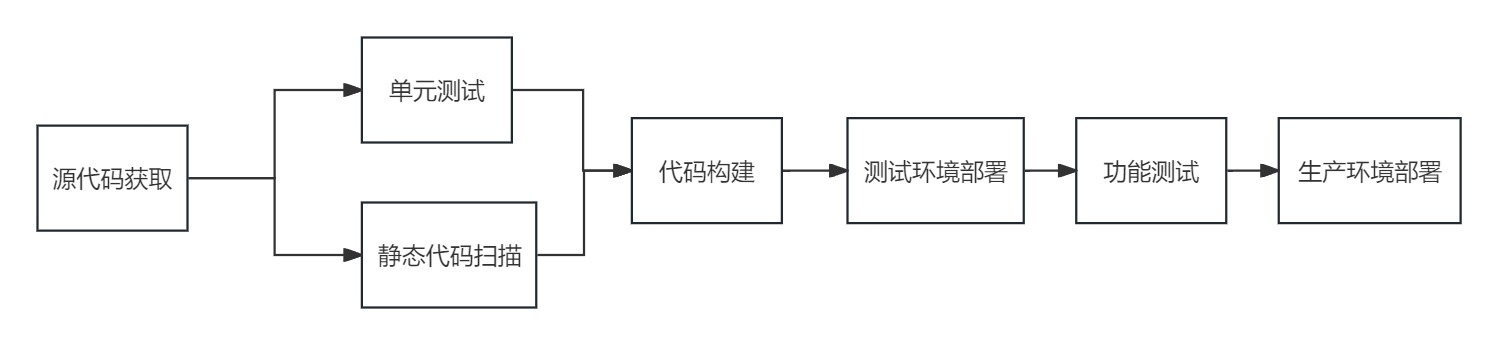
\includegraphics[width=1\textwidth]{典型流水线示意图.jpg}
    \caption{典型流水线示意图}
    \label{fig:典型流水线示意图}
  \end{figure}

CI/CD流水线使得软件的开发、测试和交付变得更加高效、可靠和可控\cite{mohammad2016continuous}。
同时,这种自动化的流程有助于加速软件交付周期,减少人工操作带来的错误,并提高整体团队的协作效率。

\section{Docker容器化技术}
容器化技术是一种轻量级的虚拟化方法,通过将应用程序及其依赖项打包到一个独立的、可移植的容器中,实现了在不同环境中一致性的部署和运行。
基于Docker的容器化技术在这一领域取得了显著的成功。

Docker 是一个由 Golang 语言开发的,开源的容器化平台,它采用了操作系统层面的虚拟化技术,允许开发人员将应用程序及其所有依赖项打包为一个称为容器的标准单元\cite{第二章Docker}。
这个容器包括应用程序的代码、运行时、系统工具、系统库和设置,确保在不同的环境中能够以一致的方式运行。

Docker容器与传统的虚拟机技术(VM)有一定相似之处,但又拥有着一系列优势。首先,Docker 容器在资源利用率方面表现出色\cite{张忠琳2014基于}。与传统虚拟机相比,它们不需要为每个虚拟机加载一个完整的操作系统,而是与宿主机共享核心,这大大减少了硬盘使用、内存占用和启动时间。
此外,Docker 容器提供了更高的效率和更快的部署速度,使得在几秒钟内就可以创建和启动容器,而虚拟机可能需要几分钟\cite{JSJY201704001}。
Docker 容器还促进了环境一致性,确保应用程序在开发、测试和生产环境中运行时的一致性和可预测性。
最后,Docker 的生态系统和工具链提供了广泛的支持\cite{DGJB201806026},包括容器编排、管理和安全,这些都是在现代云原生应用开发中不可或缺的部分。
Docker容器与传统虚拟机的对比如表~\ref{tab:Docker容器与传统虚拟机对比}所示。

\begin{table}[h]
  \centering
  \caption{Docker容器与传统虚拟机对比}
  \label{tab:Docker容器与传统虚拟机对比}
  \begin{tabular}{lcc}
    \toprule
      特性           & Docker 容器            & 传统虚拟机               \\
    \midrule
      启动时间       & 秒级                   & 分钟级                   \\
      硬盘使用       & 一般为MB               & 一般为GB                  \\
      性能           & 接近原生               & 较低   \\
      资源占用       & 低                     & 高                       \\
      系统支持数量   & 单机支持上千个容器       & 一般为几十个              \\
      部署速度       & 快                     & 慢                        \\
      环境一致性     & 高                     & 中等,受到底层VM配置的影响  \\
    \bottomrule
  \end{tabular}
  \end{table}

Docker中有两个基本概念:镜像和容器,这是CI/CD系统实现容器化的基础\cite{boettiger2015introduction}。

Docker 镜像是一个轻量级、可执行的软件包,包含了应用程序的代码、运行时、系统工具、系统库和设置。
镜像的构建规则通过 Dockerfile 文件定义,形成一个静态的快照,具有版本控制和分层结构,确保了构建的可重复性和高效性。
这些镜像可以被推送到 Docker 镜像仓库,以供后续的CI/CD环节使用。

Docker 容器是基于 Docker 镜像运行的实例,拥有独立的命名空间、进程空间、文件系统、网络配置和用户ID空间,提供了一个隔离的执行环境。
每个容器都是独立的运行单元,可以快速启动、停止和删除。
容器解决了环境一致性的问题,确保应用程序在不同的阶段和环境中能够以相同的方式运行。
容器的快速部署和回滚特性加速了CI/CD流程,使得团队能够更灵活、高效地进行应用程序的开发、测试和部署。

以下是 Docker 的关键特点和为何它适用于CI/CD系统的原因:

\paragraph{轻量级}Docker容器比虚拟机更轻量,容器的启动与销毁都是秒级,同时占用更少的资源。

\paragraph{一致性}Docker提供一致的运行环境,当Docker镜像被打包好以后,所有根据该镜像启动的容器拥有完全一致、标准化的环境。

\paragraph{可移植性}Docker容器可以在任何支持 Docker 引擎的环境中运行,无论是开发者的本地机器、测试服务器还是生产环境。这种可移植性确保了应用程序在不同阶段和环境中的一致性,简化了部署流程。

\paragraph{隔离性}Docker提供了一定程度的隔离,每个容器都运行在独立的用户空间中,不受其他容器或宿主系统的影响。这种隔离性确保了不同的流水线作业可以并行运行,同时避免了冲突和资源争用\cite{JSJC201708006}。

\paragraph{快速构建和部署}Docker的快速构建能力使得在CI/CD过程中能够更迅速地生成新的镜像,同时容器的快速启动和停止加速了部署过程。这对于频繁进行集成和部署的 CI/CD 系统至关重要。

基于以上特性,Docker几乎成为当今Devops以及CI/CD实践中不可或缺的完美解决方案\cite{第二章Devops}。

\section{容器集群调度引擎Kubernetes}
在现代软件开发领域,Kubernetes(K8s)已经成为最受欢迎的容器集群调度引擎之一,特别是在CI/CD流程的高效实现中展示了其无与伦比的优势\cite{XTYY202012038}\cite{mahboob2021kubernetes}。

Kubernetes不仅促进了DevOps文化的快速发展,还为敏捷开发提供了坚实的技术支持,极大地提高了研发团队交付高质量软件产品的能力\cite{carrion2022kubernetes}。

Kubernetes与Docker之间的关系构成了容器化技术生态系统的核心\cite{XDDS202202023}。
Docker作为容器技术的领导者,为应用提供了轻量级和可移植的封装环境。
Kubernetes则为这些容器提供了自动化的部署、扩展和管理平台。
通过将Docker容器部署到Kubernetes集群中,开发团队能够以前所未有的灵活性和自动化水平管理服务的生命周期,包括部署、扩展和更新。这种结合最大化地利用了Docker容器的隔离性和资源轻量化的优点,并通过Kubernetes的管理能力实现了更高级的自动化操作和系统灵活性。

Kubernetes的设计理念是提供一个分布式系统友好的环境,支持多种容器工具和跨云及本地部署,这使得它成为企业实现云原生应用的关键工具。其架构中包含多个关键组件,例如控制平面、节点、Pod以及服务,这些组件共同工作以确保应用的高可用性和可扩展性,并提供了负载均衡、自我修复、服务发现和配置管理等关键功能。

在CI/CD系统中,Kubernetes提供的自动化和灵活性特性尤其突出\cite{janani2022analysis}。它能够自动化CI/CD流程的各个阶段,支持声明式配置和自动化部署,使得应用的更新和回滚过程无需人工干预。此外,Kubernetes的服务发现和负载均衡功能使得服务间的通信变得更加高效,为基于微服务架构的应用提供了坚实的基础。

Kubernetes在横向扩展和故障转移方面的能力非常出色\cite{JSSG201909023}。它可以根据应用负载自动增加或减少容器实例的数量,同时监控容器健康状态并在必要时自动替换故障容器,确保了系统的高可用性。这种弹性不仅优化了资源利用率,还支持了应用性能的维护。

Kubernetes的生态系统是其另一个显著特点,随着行业内的广泛采用,出现了大量围绕Kubernetes开发的工具和扩展,如Helm、Prometheus、Istio和Knative。这些工具和扩展进一步增强了Kubernetes的功能,支持复杂的微服务架构和无服务器计算。

综上所述,Kubernetes通过其与Docker的深度整合、对DevOps实践的支持、在自动化、扩展性和可靠性方面的优势,成为构建现代软件开发管道的理想选择。其在促进软件快速开发和迭代、提高系统稳定性和可靠性方面的能力,为企业创造了巨大的业务价值,使其在实现敏捷开发和持续集成/持续部署(CI/CD)过程中扮演了不可或缺的角色。


\section{GitLab Runner}
GitLab Runner是一个开源项目,是Gitlab中CI/CD Pipeline服务中的一个核心组件,用于运行用户定义的的CI/CD作业并发送结果回GitLab\cite{eguzo2023automating}。
用户在使用GitLab代码管理服务时,可以仓库中添加以".gitlab-ci.yaml"为后缀的文件以定义流水线的配置与结构,同时完成GitLab Runner的相关设置,即可在GitLab中使用流水线服务。

GitLab Runner的设计和实现体现了敏捷开发和研发效能的提升。它能够并行执行多个作业,并且可以根据项目的需求动态地扩展和缩减计算资源,极大地提高了资源的利用效率和作业的执行速度。此外,GitLab Runner提供了丰富的执行器选项,包括Shell、SSH、Docker等,用户可以根据自己的需求选择最合适的执行器。例如,在容器化的CI/CD流水线中,Docker执行器允许每个作业在隔离的容器环境中运行,这不仅提高了作业的安全性,也保证了环境之间的一致性。

GitLab Runner的灵活性和可扩展性使其不仅在GitLab CI的场景下发挥作用,还可以被复用到其他系统中。
借助GitLab Runner,开发团队可以构建一个高度定制化的CI/CD环境,将自动化测试、代码部署等步骤无缝集成。由于其开放性和模块化设计,GitLab Runner可以与市场上的大多数主流技术栈兼容,这意味着企业可以在不重建整个CI/CD系统的情况下,将GitLab Runner集成进现有的工作流程中。

进一步地,GitLab Runner对于提高研发效能可以起到重要作用。
它支持缓存依赖项和工件,可以显著减少构建时间,并且能够自动化执行复杂的部署策略,从而加快从开发到部署的整个过程。
同时,GitLab Runner提供了详细的日志和历史记录,使得问题定位和性能监控变得更加高效\cite{vassallo2020configuration}。

在容器化的CI/CD流水线中,GitLab Runner与Docker、Kubernetes等技术的结合尤为紧密。它不仅能够在Docker容器中运行作业,还能够在Kubernetes集群中进行作业调度,这大大增强了其在容器化环境下的适用性和效率。此外,通过与消息队列系统如RocketMQ的集成,GitLab Runner可以更好地管理作业队列,优化资源分配,进一步提高流水线的性能和稳定性。

总而言之,GitLab Runner不仅是实现持续集成、持续交付的关键组件,它的高度可配置性和强大功能也使其成为了连接开发、测试和部署各环节的重要纽带。通过充分利用GitLab Runner,企业不仅能够构建高效、可靠的CI/CD流水线,还能够提升整个软件开发生命周期的质量和效率。因此,在自研的CI/CD流水线系统中深入整合和优化GitLab Runner,将为实现更敏捷、更高效的研发流程提供坚实的基础。


\section{消息队列RocketMQ}
RocketMQ是由阿里巴巴最初开发,并于2016年捐赠给Apache软件基金会的开源分布式消息队列中间件。
所谓消息队列,是一种遵循先进先出规则的高级数据结构,生产者将消息推送到消息队列中,消费者则按照次序从消息队列中获取消息,RocketMQ就是消息队列的一种。
相比与其他消息队列中间件,RocketMQ在处理重复消费、延迟消息、顺序性消息和延迟消息上有着独特的解决方案,是现今最广泛使用的消息中间件之一\cite{分布式消息系统研究综述}。

RocketMQ具备高可靠、高性能、高可用等特点。它支持丰富的消息通信模式,包括顺序消息、延时消息和批量消息等,满足不同场景下的消息处理需求\cite{RJSJ201811013}。
在容器化CI/CD流水线中,这些特性使得RocketMQ成为连接各个组件、传递任务指令和状态信息的理想选择\cite{1023416528.nh}。
通过利用RocketMQ,开发团队可以确保代码提交后的各项任务,如构建、测试和部署能够准确无误且高效地执行。

RocketMQ的高扩展性和高可用性对于构建现代化的CI/CD系统尤为重要。它能够支持上万亿级别的消息堆积,为系统提供强大的数据处理能力。此外,RocketMQ的分布式特性意味着它能够在不同的服务器节点间自动分配消息,实现负载均衡,并且在节点发生故障时,能够快速进行故障转移,保证CI/CD流水线的高可用性和稳定性。

在敏捷开发的环境下,开发、测试和部署过程频繁且迭代速度快。RocketMQ的低延迟和高吞吐量特性可以确保消息在系统内部快速流转,不会成为提升研发效能的瓶颈。
此外,RocketMQ支持跨语言的客户端,这意味着不同的服务可以使用最适合自己的技术栈,同时能够通过RocketMQ高效地进行通信。

对于任务调度而言,RocketMQ提供了稳定可靠的消息保障机制。无论是在Docker容器内还是在Kubernetes集群中,RocketMQ都能保证消息的正确送达和顺序处理。
在CI/CD流水线中,各个微服务、构建任务和测试用例经常需要根据特定的顺序和条件来触发和执行,RocketMQ的消息顺序控制和消息事务功能确保了整个流程的有序性和一致性\cite{1018841702.nh}。

总结来说,RocketMQ在容器化CI/CD流水线调度系统中发挥着核心作用。它不仅提供了高效、可靠的消息服务,还支持系统的高可用性和可扩展性,是连接持续集成和持续交付各个环节的重要纽带。通过合理利用RocketMQ,可以大大提高研发团队的工作效率,加快产品从开发到上线的整个流程,同时保证系统的稳定性和可维护性。

\section{本章小结}

本章节对CI/CD流水线、Docker容器化技术、容器集群调度引擎Kubernetes、GitLab Runner以及消息队列RocketMQ等相关技术进行了详细的概述。

首先,CI/CD流水线的概念与实践为软件开发提供了一条高效、可靠、可控的自动化路径。
Docker容器化技术则在环境一致性、资源利用率、部署速度等方面带来了显著的优势。
它通过轻量级的虚拟化手段,确保了应用在开发、测试、生产等不同环境下的一致性运行,同时提升了资源的利用效率和应用的部署速度。
Kubernetes作为容器集群的调度引擎,不仅优化了容器的部署和管理,还通过其横向扩展和故障转移等能力,可以为系统提供了高可用性和高稳定性。
GitLab Runner作为GitLab CI/CD的执行器,提供了灵活的作业执行环境,支持并行执行作业、动态扩展计算资源等特性,可以为CI/CD流水线作业提供运行支持。
最后,RocketMQ作为高性能、高可靠的消息队列中间件,在容器化CI/CD流水线调度系统中扮演着消息传递的核心角色,同时完成异步和流量削峰。
以上技术各自在CI/CD系统中扮演着不可或缺的角色,并且相互协作,共同推动CI/CD流水线系统的自动化、标准化以及高效化。
% !TeX root = ../main.tex

\chapter{需求分析}

本章叙述了系统的需求分析,首先描述了系统的总体需求分析概述,并
将用户分为三个团队角色进行了需求导出,最后从功能性和非功能性两个方面阐述了系统需要达到的目标。

\section{系统概述}
容器化 CI/CD 流水线调度系统是一个自动化的工具,旨在提高软件开发的效率和速度。
它通过自动化编译、测试和部署过程,实现持续集成和持续交付。
该系统将支持敏捷开发的实践,通过自动化任务调度来优化研发团队的工作流程。
\section{需求导出}

首先,我们要明确我们的目标是设计一个高效、灵活且可靠的容器化CI/CD流水线调度系统。
该系统不仅要能够让用户根据自己的需求高度定制化自己的流水线,并提供稳定的执行,而且还要确保这一过程尽可能自动化,减少手动干预,提高开发效率和代码质量。
此外,系统还需要能够适应不断变化的开发需求,支持快速迭代,以满足敏捷开发的要求。

在了解这些基本目标之后,本文通过与企业内各个利益相关者的深入访谈,识别出了以下具体需求:

\subsubsection{开发团队需求}
开发团队期望系统能提供一站式服务,自动完成从代码提交到部署的整个流程。
并且对系统的定制性有一定要求,开发团队希望流水线系统支持丰富的功能支持,以便满足多样化的需求。
同时开发人员希望流水线中的拓扑结构能够以图块拖拽的形式进行组合,以便开发人员能够以最高的效率完成流水线的定义与配置,从而将更多精力投入到开发工作本身。

\subsubsection{测试团队需求}
测试团队希望流水线平台能够充分自动化,以缓解测试的人力资源需求,希望系统能够自动执行各种测试,包括单元测试、集成测试和性能测试等;
同时希望系统能够生成详细的测试报告,帮助测试人员快速发现和跟踪问题。

\subsubsection{运维团队需求}
运维团队更加注重功能性和稳定性。运维团队希望系统支持庞大而复杂的流水线,以支持企业软件栈全面的集成与交付。
同时希望流水线能够支持一系列的人工操作,以便在流水线的执行过程中对流水线进行干预和把控。
稳定性方面,由于企业内存在周期性的发布高峰,运维团队希望系统能够应对高峰期时的突发流量,并且出现异常时能快速恢复,以保证高可用性。

结合以上需求,我们希望能够设计出一个不仅功能强大,而且可用性强、稳定可靠的CI/CD流水线调度系统。

\section{功能性需求}

\subsection{术语描述}
为了清晰地描述系统需求,首先需要对CI/CD流水线中一些基本术语进行解释:

\subsubsection{任务(Task)}
任务表示流水线中执行的一个单独的、不可再分的原子任务。
一个原子任务只完成一件事,如拉取Gitlab仓库代码、开源合规扫描、执行一个Shell脚本等。
任务必须包含在作业(Job) 内,同一个作业内的任务按顺序串行执行。

\subsubsection{作业(Job)}
作业表示流水线中将要调度到执行器中执行的一系列原子任务的集合,是执行器执行的最小单位。
一个作业将运行在一个独立的运行环境中,它有以下特性:
\subparagraph{由多个任务组成;}
\subparagraph{作业内一个任务失败,则整个作业失败,其余任务将不会运行。}

\subsubsection{阶段(Stage)}
阶段是一系列作业的逻辑集合。它的存在是为了更清晰的描述和管理流水线,它有以下特性:
\subparagraph{由多个作业组成;}
\subparagraph{同一个阶段下的不同作业执行方式为并行,当某个作业失败后,其它的作业会继续运行;}
\subparagraph{阶段内一个作业失败,则整个阶段失败。}

\subsubsection{流水线(Pipeline)}
流水线是一个执行一系列作业的自动化工作流,它有以下特性:
\subparagraph{由多个阶段组成;}
\subparagraph{同一个流水线下的阶段串行执行,一个阶段失败,将不会执行后续阶段;}
\subparagraph{流水线内一个阶段失败,则该流水线失败。}

图~\ref{fig:流水线示意图}是图~\ref{fig:典型流水线示意图}的流水线按照以上概念进行的逻辑边界划分,它反映了流水线、流水线阶段、流水线作业和流水线任务的层级关系。
当该流水线被手动触发后则进入第一个阶段,该阶段包括两个作业——单元测试和静态代码检查,这两个作业将并行执行,在作业执行的过程中,每个作业内部的任务将顺序执行。
当这两个作业都成功后,流水线进入第二个阶段,再执行第二个阶段中的作业——编译并上传镜像。
以此类推,在没有人工干预的情况下,流水线将自动化地执行下去,直到某个作业执行失败则流水线失败,所有作业都执行成功则流水线成功。

\begin{figure}[h]
  \centering
  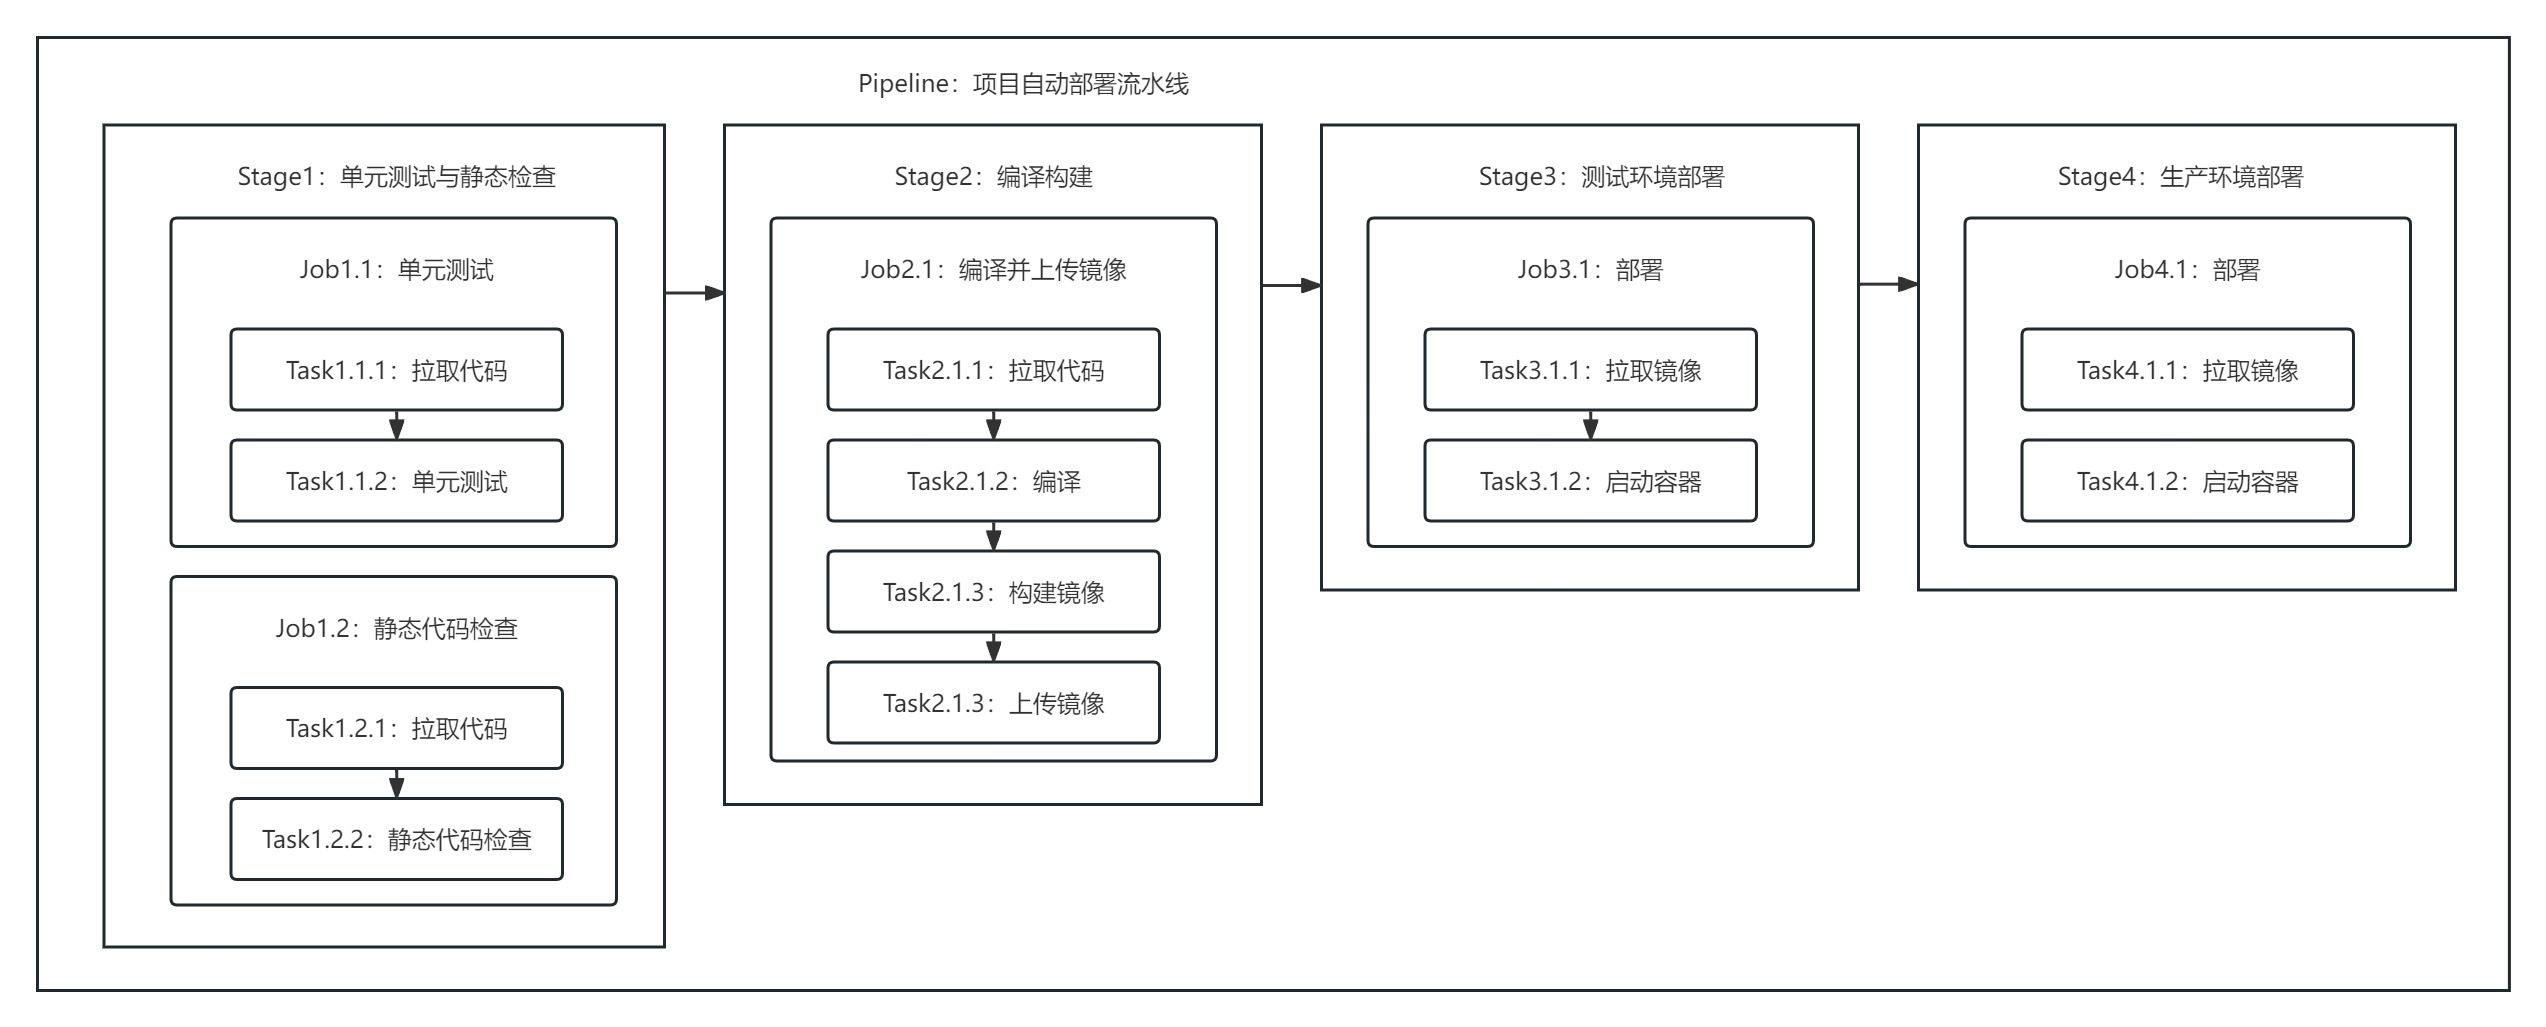
\includegraphics[width=1\textwidth]{流水线示意图.jpg}
  \caption{流水线示意图}
  \label{fig:流水线示意图}
\end{figure}

\subsection{流水线管理需求}
对于一个流水线系统来说,需要提供给用户对流水线进行增删改查的基本操作,主要包括:

\subsubsection{创建并配置流水线}
CI/CD流水线的形态十分复杂,包含了三种不同类型的子概念:阶段、作业和任务,每个子概念中又有一系列的属性需要配置,如名称、触发类型等。
创建流水线时仅仅只创建流水线是无法运行的,流水线本质上只是对流程的抽象,对其中子概念的封装,所以创建流水线的同时必须同时进行一系列配置。

在创建流水线时,用户首先需要根据其业务需求,创建出不同的子概念,比如用户想要创建一个支持编译、测试和部署的流水线,用户则可以先按顺序创建出三个流水线阶段,
再在界面中通过拖拽等方式编排各个阶段的位置,以体现不同阶段的前后顺序,再在不同的阶段里创建一系列的作业,最后在已创建的作业里创建任务,至此完成了流水线结构的创建;
然后,用户需要进行流水线配置,也就是规定流水线中各个作业和任务都要做什么事情,系统应为每个用户已创建的子概念提供表单,以便用户为各个子概念填写配置信息。

总而言之,创建流水线时,系统需要提供给用户友好的交互页面,以便用户完成流水线结构的创建与配置填写。

\subsubsection{编辑流水线配置}

系统应支持用户编辑已创建好的流水线,方便用户根据业务需求对流水线的结构和配置进行调整。

\subsubsection{查看流水线配置及其运行记录}
系统提供友好的UI界面以便用户查看流水线配置。
同时,因为一条流水线能够被反复运行,所以一条流水线会产生多次运行记录,包括当次运行的各个子概念的最终状态、运行时间、日志等等,这些运行记录也应提供入口给用户查看。

\subsubsection{删除流水线}
系统应支持用户删除不再使用的流水线。

流水线管理模块用例图如图~\ref{fig:流水线管理用例图}所示。

\begin{figure}[h]
  \centering
  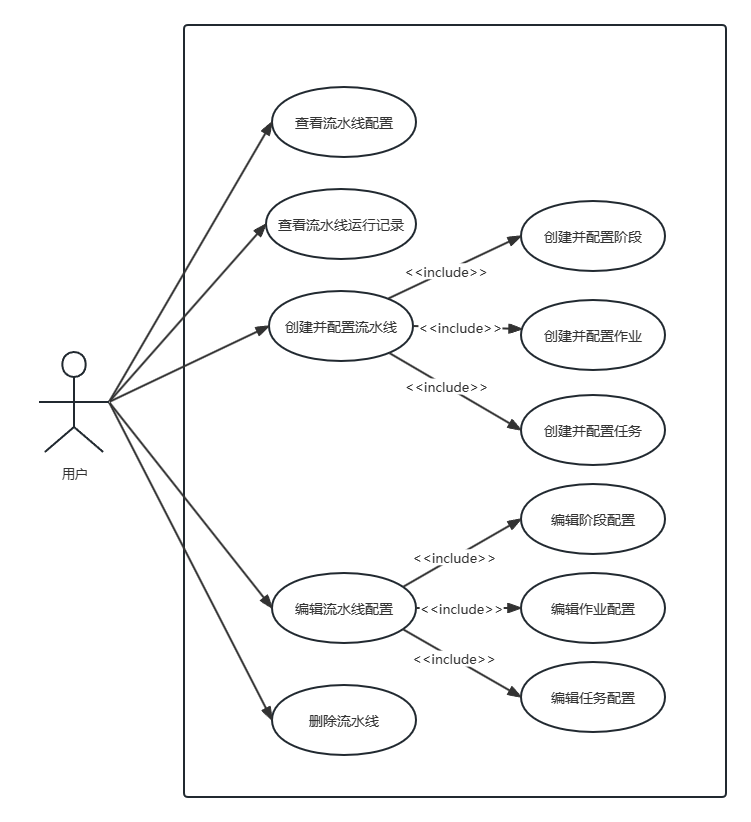
\includegraphics[width=0.7\textwidth]{流水线管理用例图.png}
  \caption{流水线管理用例图}
  \label{fig:流水线管理用例图}
\end{figure}

\subsection{人为干预流水线需求}
当用户使用已经创建好的流水线的过程中,为满足用户对流水线的复杂操作需求,提高流水线的灵活度,CI/CD调度系统需要支持用户在流水线执行过程中主动对流水线的执行情况进行干预;
干预行为主要包括:

\subsubsection{手动触发(Trigger)}
流水线的触发通常分为自动触发和手动触发两种方式

\subsubsection{取消(Cancel)}
当用户在流水线的运行过程中,意识到流水线的后续执行会产生自己不期望的后果时,CI/CD调度系统应支持用户将其取消。
注意,当阶段或作业被取消后,系统应视为其已经失败,应阻止与其串行的后续阶段或作业的继续执行。

\subsubsection{重试(Retry)}
流水线中某个作业的失败往往不是必现的,当用户认为某个失败的作业并非源于配置或者代码本身,而是因为运行环境、网络稳定性等因素导致失败时,CI/CD调度系统应支持用户将其重试。

\subsubsection{跳过(Skip)}
通常来说,一条精心配置的流水线包含非常多的阶段和作业。但复用这条流水线的各个用户的需求可能各不相同。
当某个阶段或者作业用户认为没有必要执行,或者运行时间过长用户不希望再等待时,CI/CD调度系统应支持用户将其跳过。
注意,与“取消”操作相反,当阶段或作业被跳过后,系统应视为其已经成功,应立即继续与其串行的后续阶段或作业的继续执行。

\subsubsection{人工审核(Review)}
当流水线运行到某个阶段或某个作业时,为确保后续按期望执行,并保证流水线产物的质量,CI/CD调度系统应支持用户在某个阶段或作业开始前,加入人工审核的环节。
同时,这一功能应支持流水线的编辑者自行设置审核人和审核的通过条件,比如设置了两位部门领导作为审核人,当任意一位审核人进入系统并点击“准入”后,该阶段或作业即开始执行;当两位审核人都点击“中止”后,该阶段或作业则被视为取消。

以上人工干预行为分别适用于一个或多个流水线中的子概念(流水线、阶段、作业和任务),依据对常见业务场景的分析,各个概念应支持的人工干预行为如表~\ref{tab:各个子概念应支持的人为干预行为表}:
\begin{table}[h]
  \centering
  \caption{各个子概念应支持的人为干预行为表}
  \label{tab:各个子概念应支持的人为干预行为表}
  \begin{tabular}{cl}
    \toprule
    子概念     & 人为干预行为                                     \\ 
    \midrule
    流水线     & 手动触发、取消 \\
    阶段       & 人工审核、取消、重试、仅重试阶段中失败作业   \\
    作业       & 手动触发、人工审核、取消、跳过、重试      \\
    任务       & 不允许人为干预       \\
    \bottomrule
  \end{tabular}
\end{table}

综上,得出流水线人为干预模块用例图如图~\ref{fig:流水线人工干预用例图}所示。

\begin{figure}[h]
  \centering
  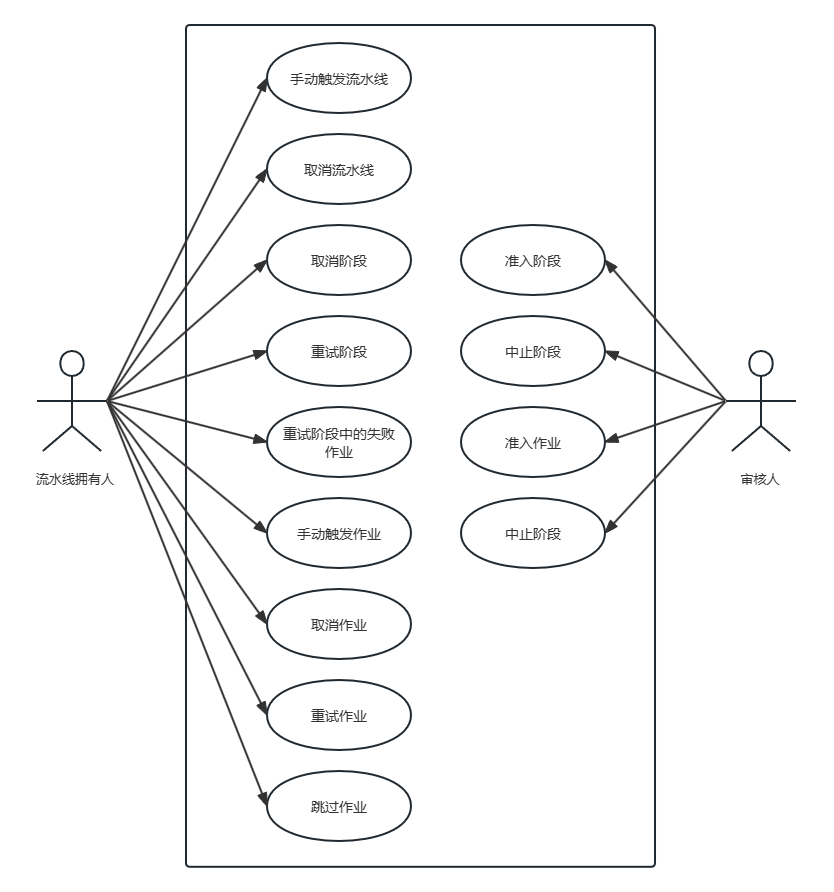
\includegraphics[width=0.8\textwidth]{流水线人工干预用例图.png}
  \caption{流水线人工干预用例图}
  \label{fig:流水线人工干预用例图}
\end{figure}

\subsection{节点管理需求}
流水线作业最终会被具象为一段脚本或者可执行文件,“节点”则是这个脚本或可执行文件的实际运行环境,
这个环境可以是物理服务器、虚拟机或者容器。
系统应允许用户主动对节点进行配置和部署,有以下几点原因:
\begin{enumerate}
  \item 适应不同作业需求。不同的作业需要的资源配置可能会有较大差异,比如AI的训练与推理对实际运行环境的算力资源有需求,
  用户则需要自己提供并指定一台带有对应硬件设备的服务器,并在系统中注册为节点以保证AI的训练与推理作业能够顺利完成。
  允许用户自定义节点能够确保每个项目能够在最适合其需求的环境中运行,从而提高构建和部署的效率。
  \item 环境隔离。并不是所有的作业都适合在虚拟机或者容器化的环境中运行,在某些场景下,特定的任务可能需要在隔离的物理机环境中运行以满足安全性要求。
  用户自定义节点允许为这些任务创建特定的安全配置和隔离环境。
  \item 提高灵活性和可扩展性。自定义的节点可以保证系统能够适应快速变化的技术和业务需求,支持新技术的快速集成和应用。
\end{enumerate}

用户对节点的管理主要包括如下内容:
\subsubsection{注册节点}
节点注册是将新节点引入系统的过程,系统为用户提供预设的配置模板,用户填写对应节点的IP、端口、标签(Tag)、环境变量、部署类型等选项后,该节点将被注册到系统中,供后续部署上线。

\subsubsection{一键部署}
为了充分降低用户使用成本,系统应提供节点的一键部署功能。
用户可以一键将系统的执行器远程部署到目标服务器,并自动完成与本系统的对接。
这项功能减少了配置新节点所需的手动操作,提高了部署效率,大幅提高系统的可用性。

\subsubsection{节点上下线}
此功能允许节点根据系统负载和维护计划自动或手动地切换其活动状态。上线的节点准备接受新任务,而下线的节点则不再分配新任务,已有任务继续执行至完成。
这样的机制确保了系统能够在不同的运行条件下维持最优的资源利用和稳定性。

\subsubsection{删除节点}
删除节点功能使得管理员能够从系统中移除不再需要或过时的节点,包括清理与这些节点相关的配置信息和数据。这不仅有助于资源的合理管理,也保持了系统的整洁性和高效运行。

节点管理的用例图如图~ \ref{fig:节点管理用例图}所示。
\begin{figure}[h]
  \centering
  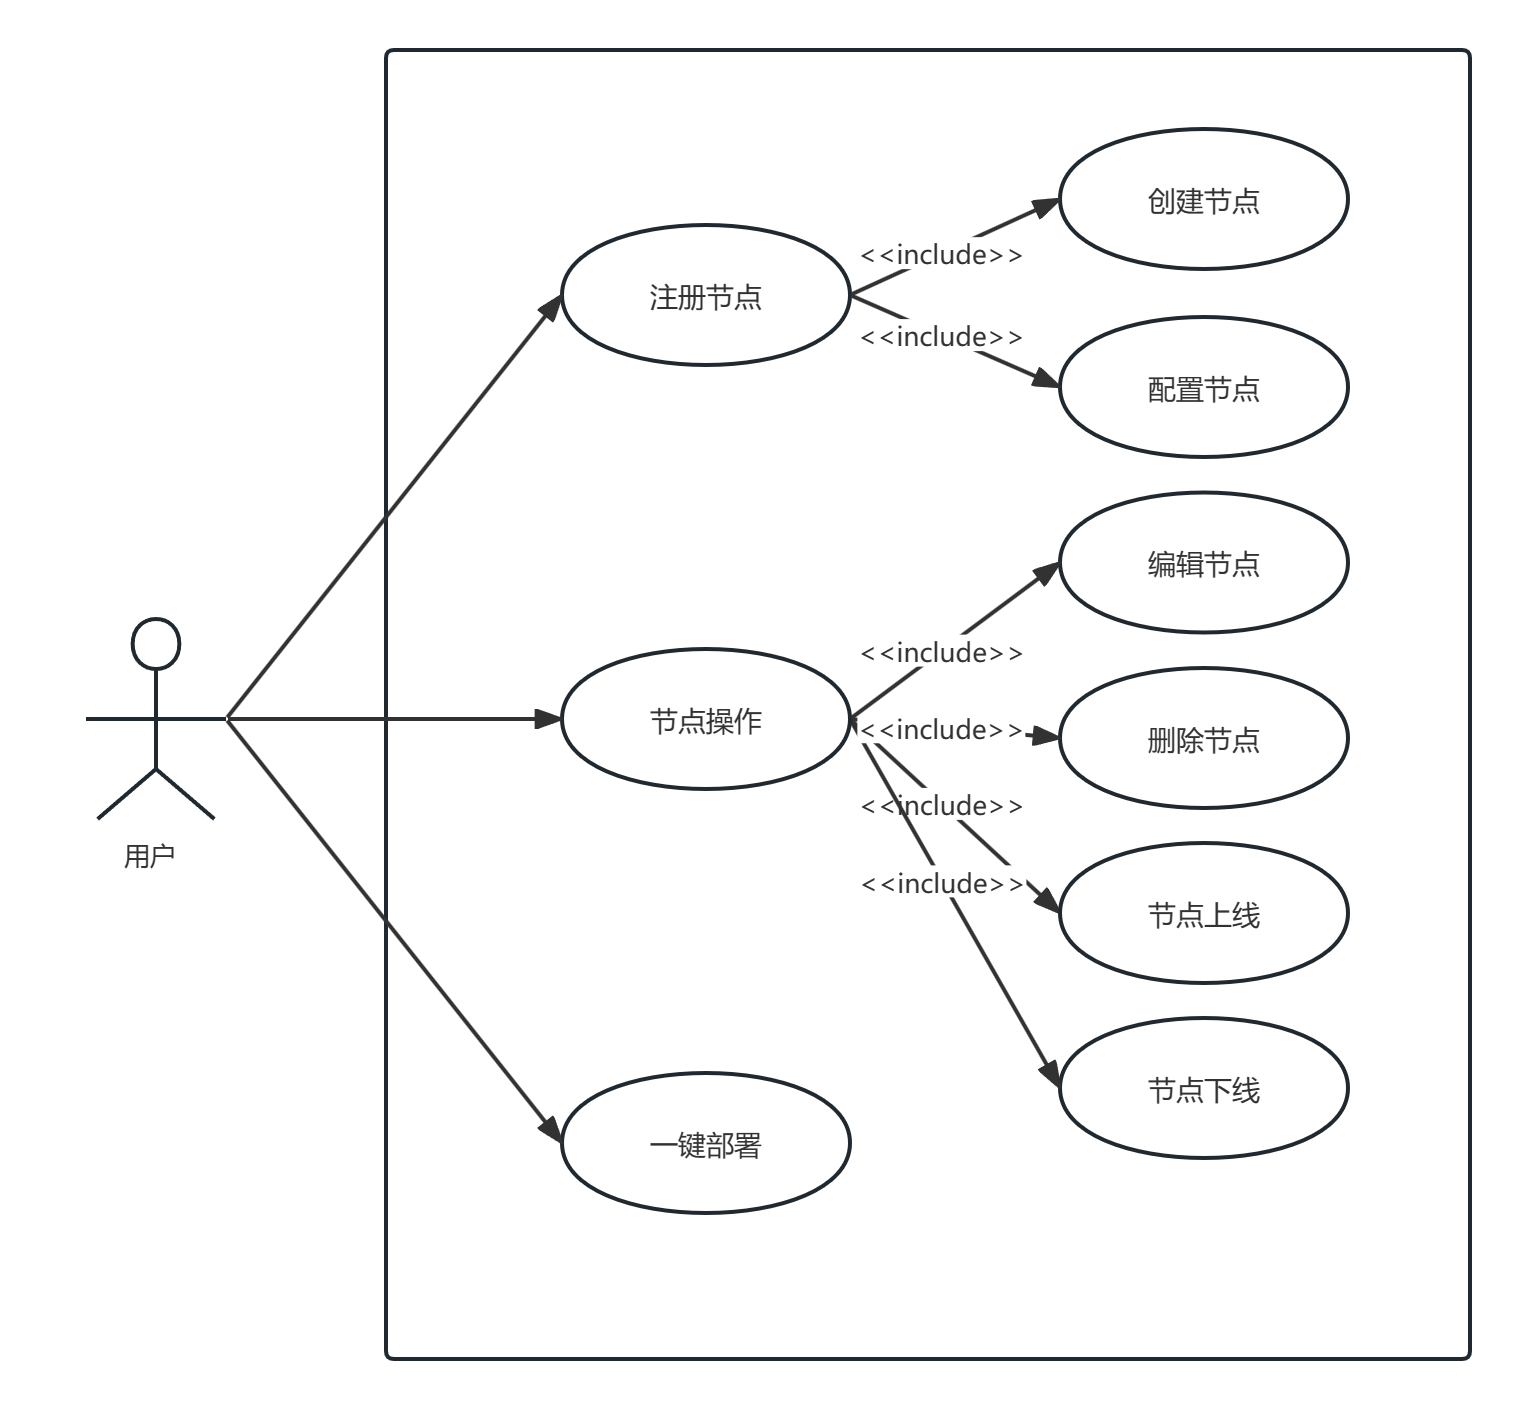
\includegraphics[width=0.7\textwidth]{节点管理用例图.png}
  \caption{节点管理用例图}
  \label{fig:节点管理用例图}
\end{figure}

\subsection{Docker镜像管理需求}
在CI/CD流水线系统中,绝大多数流水线运行的作业都是通过Docker容器进行的,这直接要求系统必须提供多样化的Docker镜像以供用户选择,以满足不同作业的运行需求。
镜像管理因此成为系统执行多样化的作业的重要前置功能,负责镜像的制作、上传、删除和详情查看等功能。
有效的镜像管理不仅保障了容器化作业的顺利执行,也提高了整个系统的灵活性和可用性。

用户对Docker镜像的管理主要包含以下内容:

\subsubsection{镜像制作}
镜像制作的自动化和安全化是镜像管理的核心。本系统应提供两种制作镜像的方法:

一是通过DockerFile构建,这种方式为高度自动化和定制化的镜像制作提供了可能,用户通过编写DockerFile来定义镜像的构建过程。这要求用户对DockerFile的语法和构建过程有深入理解。
二是使用commit提交,这种方式适用于需要手动环境配置的场景,通过将运行中的容器状态提交为新的镜像。这种方法依赖于SSH协议远程连接容器,保障了操作的安全性。

\subsubsection{镜像删除}
考虑到存储资源的有效利用,镜像删除功能是镜像管理不可或缺的一部分。本系统通过引入引用计数机制,确保不再被需要的镜像能够被有效清理,释放存储空间,同时解决了传统删除机制无法彻底删除底层文件的问题。

\subsubsection{镜像上传}
镜像上传过程中维护Layer引用记录文件的完整性和准确性是镜像管理的另一关键点。这一机制确保了镜像仓库的数据一致性和完整性,特别是在镜像频繁更新的环境下尤为重要。

镜像管理的用例图如图~ \ref{fig:镜像管理用例图}所示。

\begin{figure}[h]
  \centering
  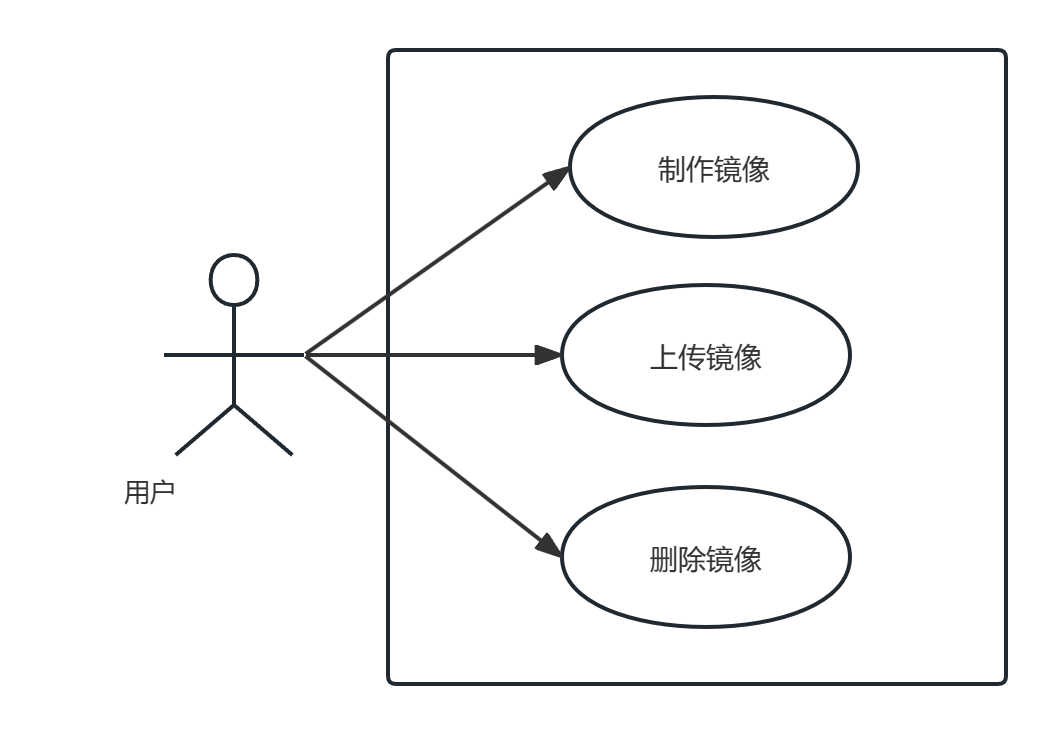
\includegraphics[width=0.7\textwidth]{镜像管理用例图.png}
  \caption{镜像管理用例图}
  \label{fig:镜像管理用例图}
\end{figure}

% \subsection{插件化需求}
% CI/CD流水线系统的最终目的是提高企业用户的开发效率。
% 市面上现有的持续集成系统,在用户配置流水线的作业时,往往只有系统预置的一些功能模块可供选择,大大限制了系统的灵活性;
% 又或是需要用户亲自进行大量的配置和脚本编写,以满足一条复杂流水线中不同作业的需求。
% 为处理这种灵活性与效率之间的矛盾,插件化是一种很好解决方式,系统管理团队将会预提供一个丰富多样的插件库,同时也需支持用户自行定义插件,自用或发布到插件市场中。
% 如此一来,当用户构建一条流水线时,可以根据自己选择不同的插件来组合成流水线作业,从而快速完成流水线的配置。

% 插件市场中主要包含如下内容:

% \subsubsection{插件管理}
% 在CI/CD系统中,插件本质上是对一套配置清单和一个执行脚本的抽象,这种设计旨在简化插件的使用和集成过程,使用户能够通过填写配置清单来定制插件行为,然后执行脚本以在CI/CD流程中实现特定功能。
% 系统应让用户能够轻松管理和编写自己的自定义插件,同时提供一种机制,使用户能够编辑出属于该插件的配置清单(即使用该插件时需要填写的配置信息),并确保脚本的安全、有效执行。
% 同时,系统应支持插件的版本管理。每当插件更新时,应记录版本历史,允许用户选择特定版本进行安装。如果新版本存在问题,这一机制确保了用户可以轻松回退到旧版本。

% \subsubsection{插件发布}
% 开发者在自定义插件并满足个人或团队需求后,可以选择将其发布到插件市场中,供其他用户使用。
% 发布流程应简洁明了,并支持插件的描述、分类和版本信息定义。

% \subsubsection{插件审核}
% 安全性是插件市场的重要考虑因素。
% 市场应该只托管经过审核的插件,确保不含有恶意代码或存在安全漏洞,未经审核的插件一旦在节点中运行,可能会对系统安全产生影响。
% 插件的发布和版本更新应由指定的审核人进行通过或驳回。

% 插件市场的用例图如图~ \ref{fig:插件市场用例图}所示。

% \begin{figure}[h]
%   \centering
%   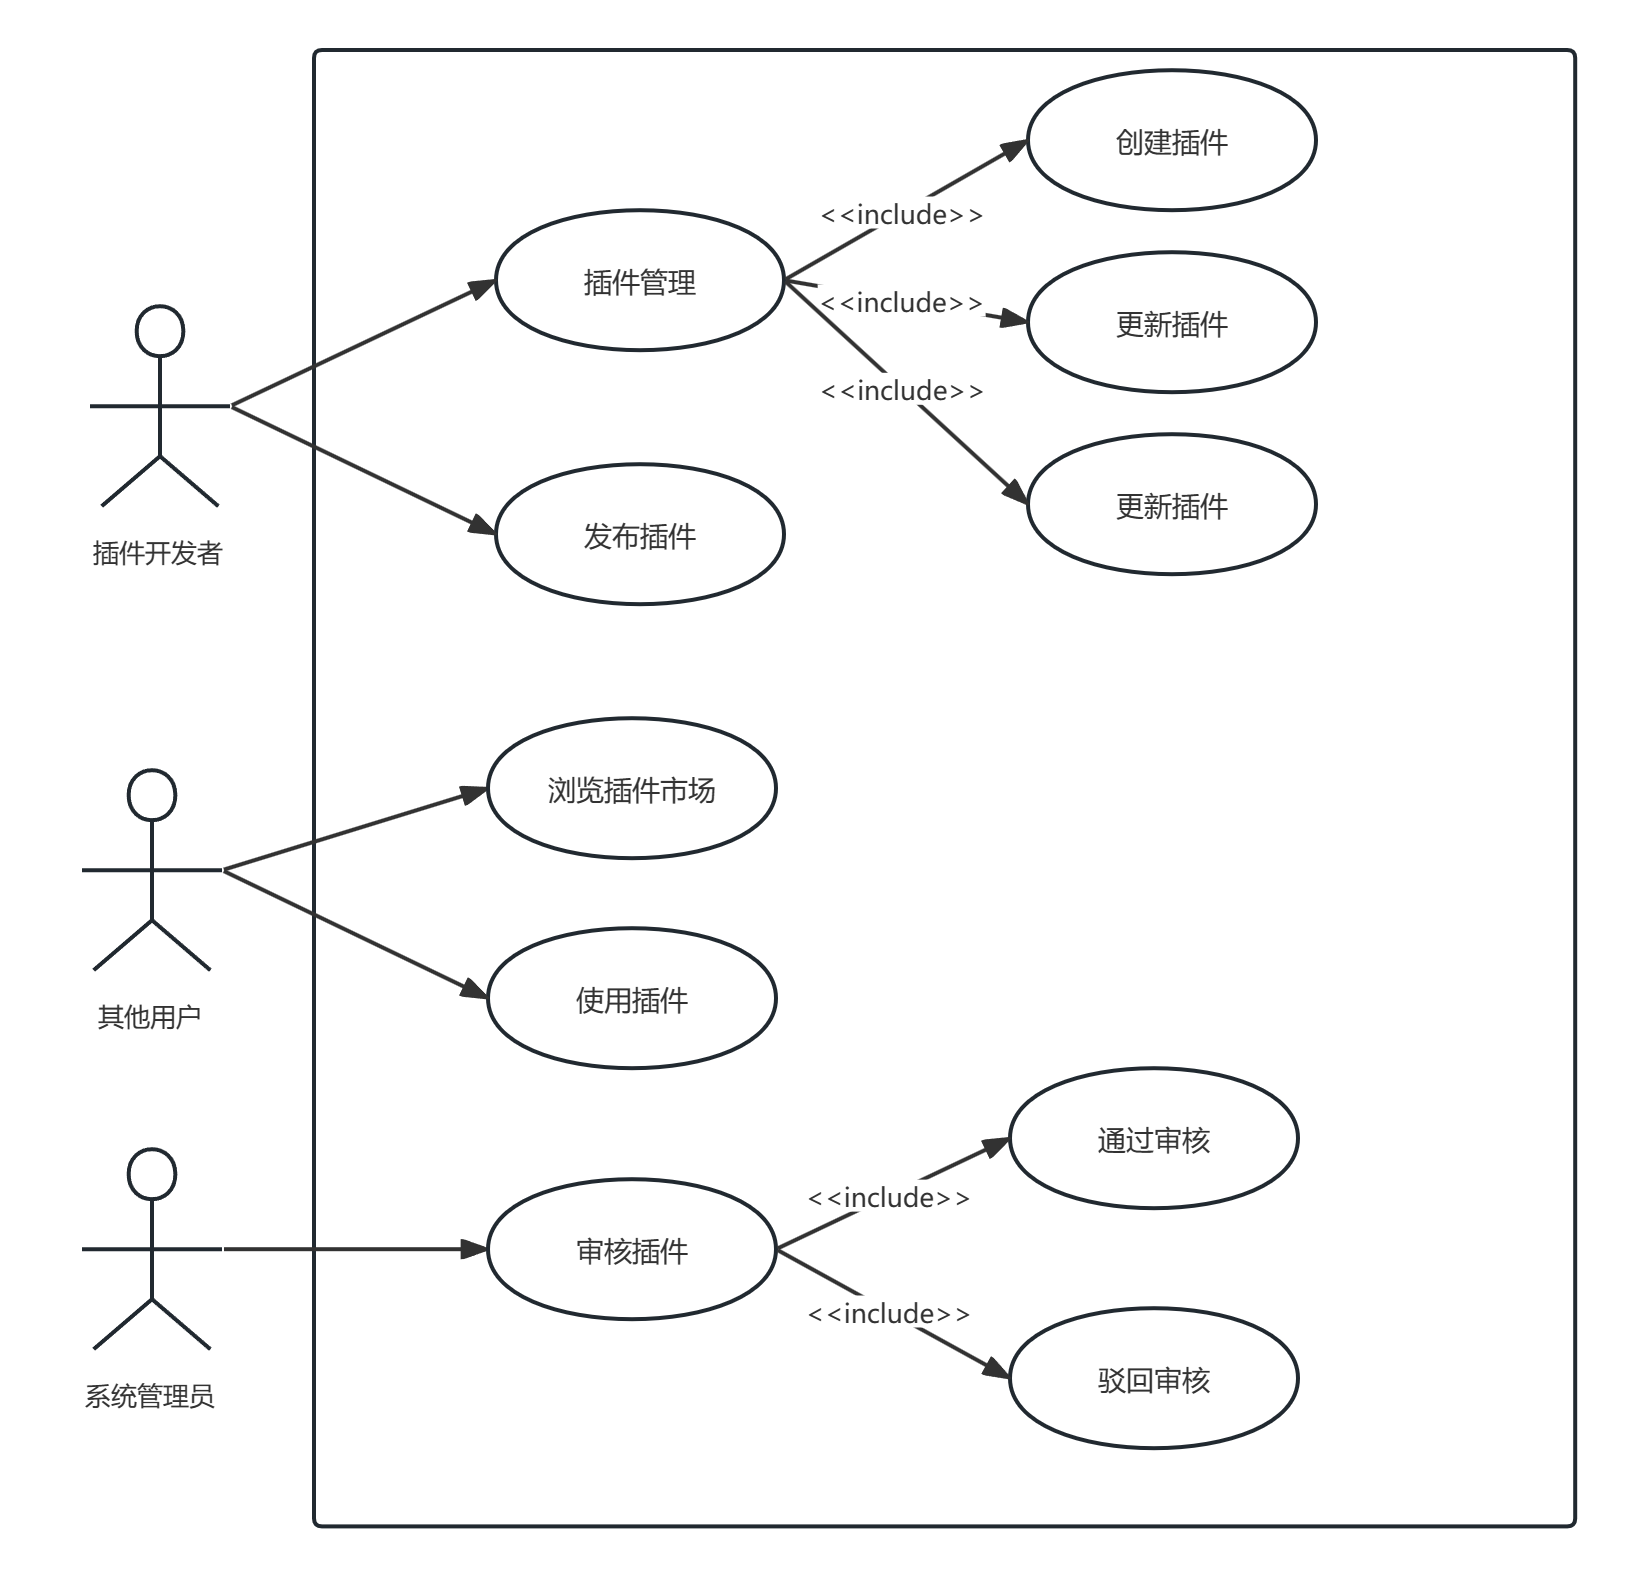
\includegraphics[width=0.7\textwidth]{插件市场用例图.png}
%   \caption{插件市场用例图}
%   \label{fig:插件市场用例图}
% \end{figure}

\subsection{状态流转需求}
在流水线的执行过程中,流水线中的每个子概念都在不同的状态间流转,通常来说应有如下状态:
就绪中(Pending)、执行中(Running)、执行成功(Success)、执行失败(Failed)、被跳过(Skipped)、被取消(Canceled)。

CI/CD调度系统需要保障流水线作业能够进行正确的状态流转,以保证用户能够正确、及时地得知流水线的执行情况。
同时,状态的正确流转也是流水线能按照正确逻辑链路执行的保证,系统需要结合当前流水线内各个子概念的状态,结合用户的人为操作,来判断流水线接下来的状态。

\subsection{流水线作业合理调度需求}
\label{subsec:流水线作业合理调度需求}

作业是流水线执行器中执行的最小单位,CI/CD调度器作为流水线配置与作业实际执行环境的中间环节,需要从作业排队、一致性分发、统一调度等方面保证作业的合理调度。

首先,系统需要保证作业的执行顺序与其被调度的顺序一致,即先来先执行。其次,当相当数量的作业被调度,超过了执行器的承载能力时,系统应能保证作业的阻塞等待,当前执行的作业结束执行后,再执行阻塞中的作业。
以上两点需求业内往往借助开源的消息队列服务实现,如RocketMQ等,借助消息队列先进先出和持久化的特性,保证了作业的调度顺序和阻塞等待。

然后,系统需要完成流水线作业的分配任务,将作业能够合理的分配给不同的作业执行模块。
当调度器判断应该调度某个作业时,CI/CD调度器将根据流水线配置时用户预填写的内容封装作业信息,再交付给执行器执行任务。
这一特性往往通过消息队列中消息的Tag和Title概念来实现对作业的精确分配。
同时,系统需要能够保证一个作业只能被一个执行器所执行,不能被多个执行器重复执行。


\section{非功能性需求}

除功能性需求外,系统需要满足以下非功能需求:

\subsubsection{高性能}
本系统致力于提升效能,提高用户的研发效率,需要保证优秀的性能和较短的响应时间。
当用户进行流水线管理时,对流水线配置的增删改查应在2s内完成;
当用户人为干预流水线时,系统应在2s内给予用户反馈;
当流水线中阶段、作业或者任务的状态发生改变时,应在5s内对用户进行展示。

\subsubsection{高稳定性}
CI/CD流水线系统的可靠性和稳定性尤为重要,一旦系统发生故障则直接影响整个企业的开发人员、测试人员和运维人员,阻塞代码合并、业务提测、系统发布等流程。
本系统可以借助以Kubernetes为代表的容器编排系统,实现横向扩展和故障转移的能力,以保证系统在使用高峰期时的稳定性。

\subsubsection{高可用性}
CI/CD在当今的软件开发流程中是不可缺少的一环,系统应尽量保证7×24小时的服务提供。
依据业界常用指标,本系统需要至少达到99.99\%的可用性。
换算成服务时间则根据公式:服务可用率=成功调用数/总调用数,系统每一年的时间内,无法提供服务的总时间不能超过52分钟。

\subsubsection{高易用性}
本系统应提供友好的交互逻辑,让缺乏相关知识背景的用户能够快速找到流水线的编辑与配置方式;
同时,由于CI/CD流水线通常有着复杂的层级与结构,系统应提供所见即所得的流水线拓扑结构界面,以便用户查看和调整;
最后,流水线的执行过程中应提供入口,将各个作业的运行日志可视化地展示给用户,方便用户时刻监控流水线作业的执行情况。

\subsubsection{高安全性}
流水线一旦执行,可能会对其对应的系统产生影响,如发布新版本、发送通知等等。
为避免产生不期望的后果,系统应对流水线的触发以及各种操作进行严格的权限控制。
比如对某一条流水线的任何人为干预操作都应该由只能由流水线的归属人执行,其他人操作则提示无权限。


\section{本章小结}

本章对容器化CI/CD流水线调度系统进行了全面的需求分析,包括系统概述、功能性需求与非功能性需求。

首先,系统需求从开发、测试和运维团队的具体需求出发,明确了系统设计的高度定制化、自动化和灵活性需求。
通过深入访谈与分析,细化出流水线管理、人为干预、节点管理、Docker镜像管理及状态流转等关键功能性需求,确保系统能够满足多样化的研发流程并提升研发效能。

在非功能性需求方面,系统强调了高性能、高稳定性、高可用性、高易用性和高安全性的重要性。
这些要求保证了系统不仅在功能上能够满足用户的需求,同时也在性能和可靠性上达到企业级应用的标准。

总体来说,本章的需求分析为系统的设计和实现从需求侧提供了清晰的指导,确保了容器化CI/CD流水线调度系统能够高效、稳定运行,满足现代软件研发的高速迭代和自动化需求。
% !TeX root = ../main.tex

\chapter{系统概要设计}
本章叙述了CI/CD流水线调度系统的设计。
首先介绍了系统的总体设计和架构分层,随后分别叙述系统内各个模块的设计与其之间的连接,
然后后对系统的数据库从概念设计和逻辑设计两方面进行了阐述,最后对本小节内容进行了总结。

\section{系统总体设计}

在对整个CI/CD流水线调度系统进行需求分析后,可以发现本系统的功能业务复杂且对部分服务的横向扩展有着较高需求。
可将本系统的核心模块拆分为三个微服务,分别为Backend服务、调度器服务和执行器服务,每个服务下又包含一些子模块。
进行这样服务划分的目的是降低系统间各模块的耦合性,并为不同的模块分配合适的资源,方便不同的模块分别以多节点的方式进行部署。
同时,拆分后的服务借助容器调度系统Kubernetes,可以实现弹性扩容和故障转移。
系统架构图如图~ \ref{fig:系统架构图}

\begin{figure}[h]
  \centering
  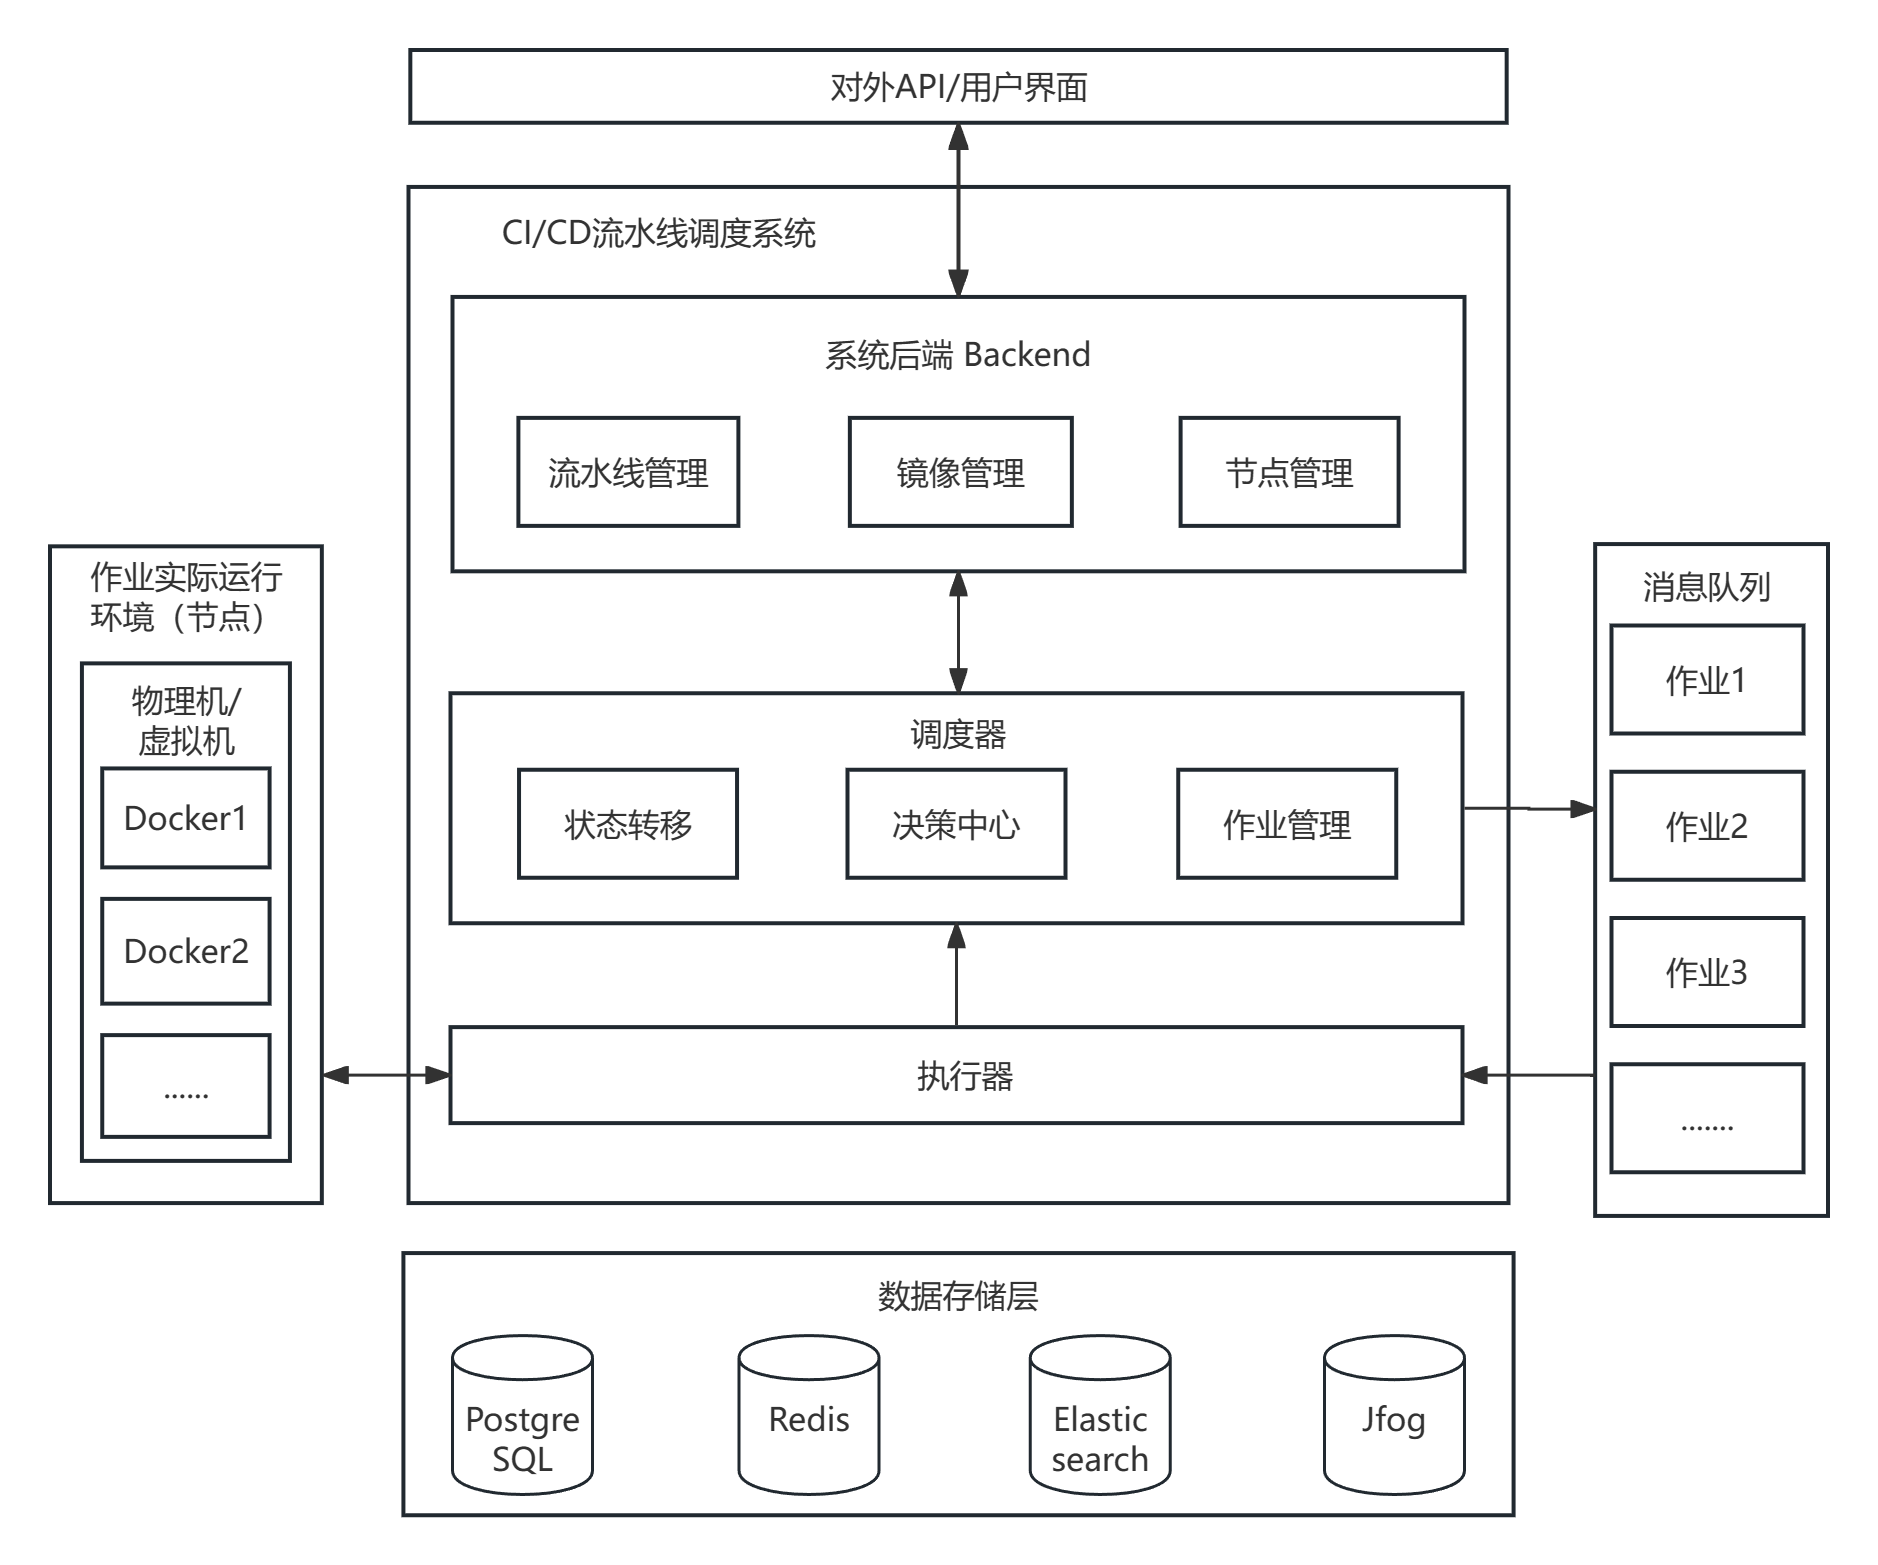
\includegraphics[width=1\textwidth]{流水线系统架构图.png}
  \caption{系统架构图}
  \label{fig:系统架构图}
\end{figure}

首先最上层是对外公开的api和前端UI,用户将通过该层与

系统内部同一时刻将有许多流水线作业同时执行,调度器负责流水线中各个子概念的状态切换,同时依据不同流水线的配置和状态来对当前流水线作业的调度进行决策,将需要被执行的作业交付给执行器模块。
执行器则最终负责各个流水线作业的真实执行,将作业转换为真正的可执行程序或者脚本后在真实的运行环境(Docker、物理机或虚拟机)中执行,并实时监控中运行环境中作业的运行状态,反馈给调度器。



\section{系统模块设计}
把每个模块讲一下:加入数据流图描述作业数据的流动。

\subsection{Backend}

首先是Backend模块,系统通过该模块向外部暴露API以供前端/外部接口调用。
用户在前端进行的操作、填写的配置信息等将通过API接口传递给Backend模块,Backend模块接收到数据后,会进行相应的业务逻辑处理,如对用户创建的流水线进行合法性校验、对作业数据进行合法性校验等,最后负责将数据落库。
同时,在流水线运行过程中,用户对流水线的手动干预操作,也是先调用接口传递给Backend模块,然后再由Backend模块进行一定处理后传递给调度器模块,用户界面与调度器模块完全解耦。

Backend有以下三种典型服务场景:

当用户通过UI界面或API接口传入如“取消”、“跳过”、“人工审核通过”等人工干预命令时,Backend会根据权限模型对用户进行鉴权,如只有流水线的拥有者才有权干预流水线、只有预设的审核人才有权进行人工审核等。
通过鉴权后,Backend将对人工干预命令进行进一步封装,携带一些额外的信息后,将命令发送给调度器模块,由调度器对流水线的执行进行真正的干预。

当用户通过UI界面或API接口创建或编辑流水线时,Backend会对流水线的内容进行解析,并通过序列化器对内容进行合法性校验,然后将流水线以阶段、作业和任务的维度进行分拆,
并将拆解后的流水线数据持久化进数据库。
同样的,用户通过UI界面或API接口进行镜像管理和节点管理时,Backend模块负责业务逻辑处理、数据持久化以及与镜像服务器或节点服务器之间的交互等。

当用户通过UI界面或API接口触发流水线时,Backend将从数据库中获取流水线数据,进行一定封装后发送给调度器模块。
随后,调度器会不断地向Backend返回流水线的执行信息,以便Backend实时更新流水线的运行状态。
与此同时,Backend会接收到前端的轮询请求,用以实时展示给用户。

\subsection{调度器}

调度器模块是整个系统的核心模块,其中包含状态转移、决策中心与作业管理三个子模块,分别介绍如下:

\subsubsection{状态转移}

对流水线、阶段、作业和任务的状态维护至关重要,一来用户需要实时观察流水线中各个子概念的状态,以便实时知晓运行情况;
二来子概念的状态是流水线中进行下一步决策的重要判定依据,例如只有一个阶段中的所有作业都被置为成功,阶段的状态才会变为成功,只有当阶段被置为成功,且下一个阶段是准入的,才会触发写一个阶段的执行。
依据需求分析,结合对目前市面常见CI/CD平台的参考,系统中设计了就绪中(Pending)、执行中(Running)、执行成功(Success)、执行失败(Failed)、被跳过(Skipped)、被取消(Canceled)六种状态。
各个状态的具体解释如表~\ref{tab:状态解释表}。
\begin{table}[h]
  \centering
  \caption{状态解释表}
  \label{tab:状态解释表}
  \begin{tabular}{cl}
    \toprule
    状态           & 解释                                     \\
    \midrule
    就绪中         & 一切准备工作就绪,等待被自动执行、手动执行或审核通过\\
    执行中         & 正在被执行                 \\
    执行成功       & 顺利执行完毕后的状态        \\
    执行失败       & 执行过程中出错后的状态       \\
    被跳过         & 被用户人为干预执行“跳过”后的状态         \\
    被取消         & 被用户认为干预执行“取消”后的状态         \\
    \bottomrule
  \end{tabular}
\end{table}
以上状态适用于流水线中的各个子概念。

引起一个作业状态转移来自于两种事件,一种是来自Backend的人工干预事件,一种是执行器通知的作业成功或失败的事件。
这种根据事件或动作引起状态转移的情况,在软件工程中可以使用有限状态机(Finite State Machine,FSM)的模型来设计。
根据有限状态机的理论,我们需要识别模型中的“状态”和“事件”,状态已经在前文有所定义了,而对于作业(Job)来讲:事件则包含所有的人工干预操作:
触发、取消、跳过和重试,同时包含执行器的状态通知:成功和失败,其次还应包含人工审核的相关内容,包含审核通过和审核驳回。

作业状态机状态转移如表~\ref{tab:作业状态机状态转移表}所示。

\begin{table}[h]
  \centering
  \caption{作业状态机状态转移表}
  \label{tab:作业状态机状态转移表}
  \begin{tabular}{cll}
    \toprule
    事件           & 允许该事件的状态          & 事件发生后状态                  \\
    \midrule
    触发           & 就绪中                   & 执行中       \\
    取消           & 执行中                   & 被取消       \\
    跳过           & 执行中                   & 被跳过       \\
    重试           & 执行失败、被跳过、被取消   & 执行中       \\
    审核通过        & 就绪中                   & 执行中        \\
    审核驳回        & 就绪中                   & 执行失败       \\
    作业执行成功     & 执行中      & 执行成功   \\
    作业执行失败     & 执行中      & 执行失败   \\
    作业执行超时     & 执行中      & 执行失败   \\
    \bottomrule
  \end{tabular}
\end{table}

对于任务(Task)而言,其状态变化与作业类似,但区别在于作业时用户操作和执行器执行的最小单位,
而任务是包含于作业之中的子概念,所以当用户事件导致作业的状态发生变化时,其中任务的状态也随之改变。
例如,当用户跳过一个执行中的作业时,作业的状态应被设为被跳过,同时作业内所有的任务的状态将全部被设为被跳过,对于重试、取消、触发、审核通过和审核驳回事件同理。
而执行成功和执行失败事件来说则有所不同,由于作业中的任务是顺序执行的,所以任务与任务之间有执行的前后之分,故并不能统一进行状态修改。
对于任务来讲,执行器会独立地触发任务执行成功与任务执行失败两种事件,这是因为任务所执行的脚本本质上是整个作业所执行脚本的片段,执行器能够感知到目前已经执行的脚本是否执行成功,所以这两种事件能够独立于作业的成功与失败之外引发任务的状态变动。

任务状态机状态转移如表~\ref{tab:任务状态机状态转移表}所示。

\begin{table}[h]
  \centering
  \caption{任务状态机状态转移表}
  \label{tab:任务状态机状态转移表}
  \begin{tabular}{cll}
    \toprule
    事件           & 允许该事件的状态          & 事件发生后状态                  \\
    \midrule
    所属作业被触发           & 就绪中                   & 执行中       \\
    所属作业被取消           & 执行中                   & 被取消       \\
    所属作业被跳过           & 执行中                   & 被跳过       \\
    所属作业重试            & 执行失败、被跳过、被取消   & 执行中       \\
    所属作业审核通过        & 就绪中                   & 执行中        \\
    所属作业审核驳回        & 就绪中                   & 执行失败       \\
    任务执行成功            & 执行中      & 执行成功   \\
    任务执行失败            & 执行中      & 执行失败   \\
    作业执行超时            & 执行中      & 执行失败   \\
    \bottomrule
  \end{tabular}
\end{table}

对于阶段(stage)而言,其状态变换完全不受执行器的影响,因为执行器执行的是作业,而阶段本质上只是一套可以并行的作业的逻辑集合,
所以阶段的状态仅由该阶段中的所有作业的状态共同决定。
一般来说,我们期望阶段中最值得关注的作业状态成为整个阶段的状态,同时需要结合不同状态的特性,来设计阶段的状态转移。
,为了统一阶段状态处理逻辑,系统中引入了“状态优先级”这一概念,系统中不同状态的优先级如表\ref{tab:状态优先级表}所示。

\begin{table}[h]
  \centering
  \caption{状态优先级表}
  \label{tab:状态优先级表}
  \begin{tabular}{cl}
    \toprule
    状态           & 优先级                                     \\
    \midrule
    被跳过         & 1         \\
    执行成功       & 2         \\
    就绪中         & 3         \\
    执行中         & 4         \\
    被取消         & 5         \\
    执行失败       & 6         \\
    \bottomrule
  \end{tabular}
  \note{注:数字越大表示优先级越高}
\end{table}

当一个阶段内的任意作业的状态发生变化时,系统会将本阶段内所有作业状态中的状态优先级最高的状态设置为阶段的状态。
比如,某阶段中有三个作业,作业1和作业2处于执行成功的状态,作业3的状态为执行中,所以该阶段的状态应是优先级最高的作业3的状态,也为执行中,
这是符合逻辑的,因为阶段内存在尚未执行完的作业,所以整个阶段的状态理应处于执行中;
又比如作业1和作业2被跳过,作业3处于执行成功的状态,则整个阶段的状态为执行成功,这是因为用户跳过一个作业,说明用户并不关注该作业的执行,故赋予其最低优先级。
其余情况均可参照表\ref{tab:状态优先级表}进行判断。
系统通过这种阶段优先级的处理方式,极大简化了阶段的状态转移逻辑。
流水线的状态转移与阶段类似,根据流水线下所有阶段状态的最高优先级来确定流水线的状态,具体内容不再赘述。

\subsubsection{决策中心}
决策中心依据当前Backend传入的命令以及目前流水线中作业与任务的状态,来准确地生成事件以及事件相关活动,以下一一介绍各种事件的产生条件以及活动设计。

\paragraph{触发作业}
触发作业事件存在两种产生时机,一种是调度器收到来自Backend的触发流水线命令时,决策中心会对首个阶段中的作业一一进行处理;
另一种情况是,当一个阶段状态变更为取消或成功时,会对当前阶段的下一阶段中的所有作业进行处理。

此时需要进行一些条件判断,首先需要判断阶段和作业的准入条件,如果是自动触发,则进行下一步;
如果是手动触发,则需要等待Backend端传来手动触发阶段和作业的命令。
一旦准入条件满足,即可将作业交付给作业管理子模块,由作业管理子模块将作业交付给执行器,待执行器执行作业。

注意,以上条件满足时并不会立即产生触发作业事件,因为执行器的并行处理作业是有数量上限的,当执行器已经达到满载,多余的作业会堆积在消息队列待执行器拉取,
所以只有当决策中心收到执行器报告的执行信息时,才会发出触发作业事件。触发作业时序图如图\ref{}所示。

\begin{figure}[h]
  \centering
  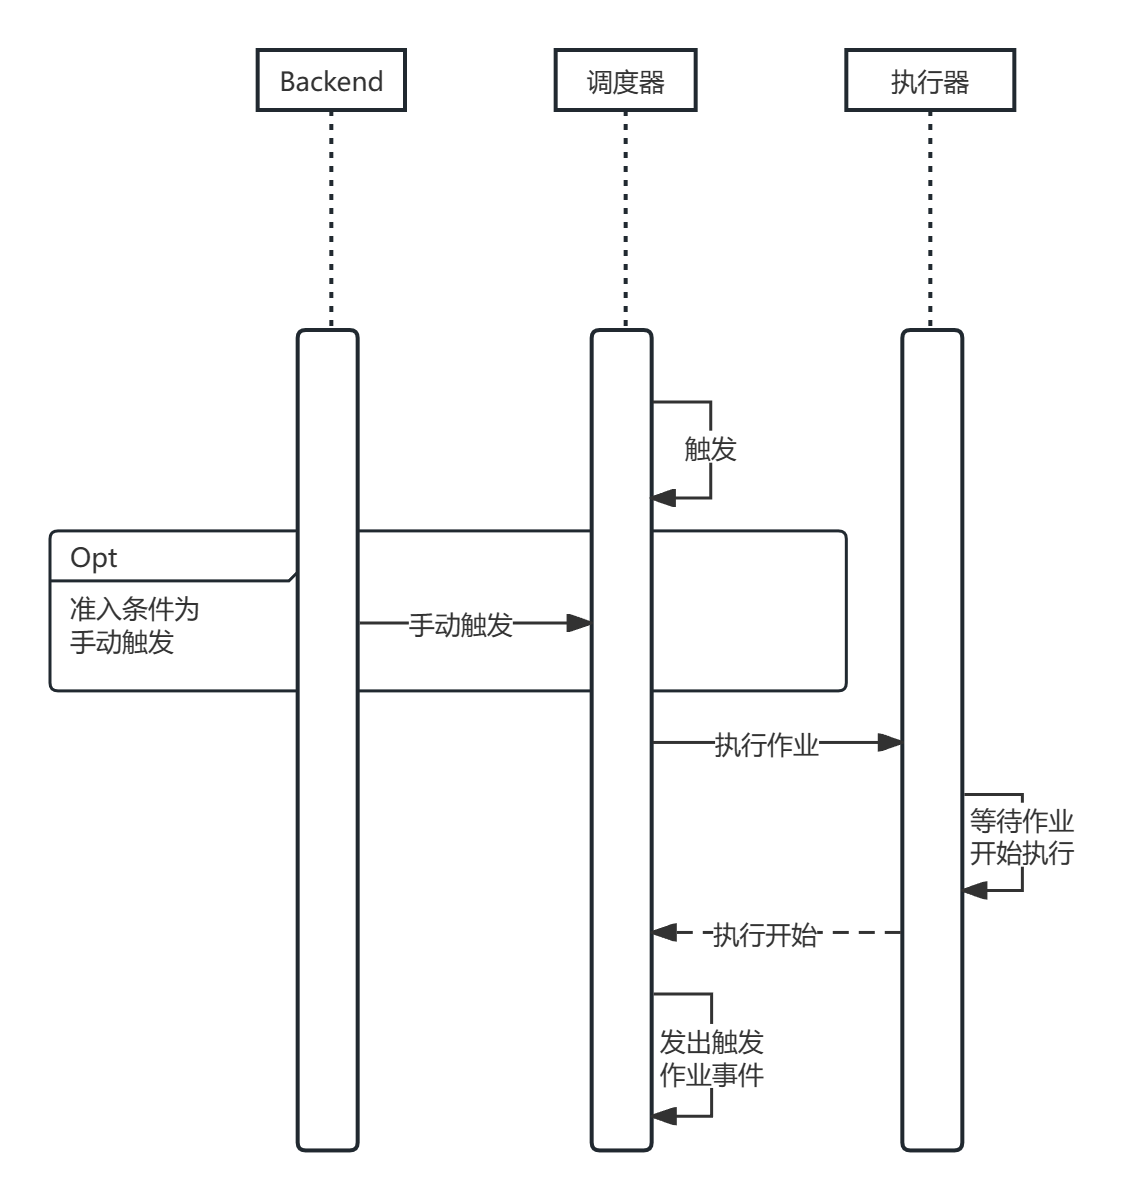
\includegraphics[width=0.8\textwidth]{触发作业时序图.png}
  \caption{触发作业时序图}
  \label{fig:触发作业时序图}
\end{figure}

\paragraph{跳过作业与取消作业}
在决策中心层面,跳过作业与取消作业的活动类似,只不过转移后的状态不同。
当决策中心收到Backend发出的跳过或取消作业的命令时,首先判断任务状态是否为执行中,只有任务状态为执行中时才允许跳过与取消。
然后决策中心将发出跳过或取消事件交由作业状态机进行状态流转,此后需要调度器主动向执行器发出一个中止作业的命令,避免执行器继续执行作业,浪费系统资源。

跳过作业与取消作业时序图如图\ref{}所示。

\begin{figure}[h]
  \centering
  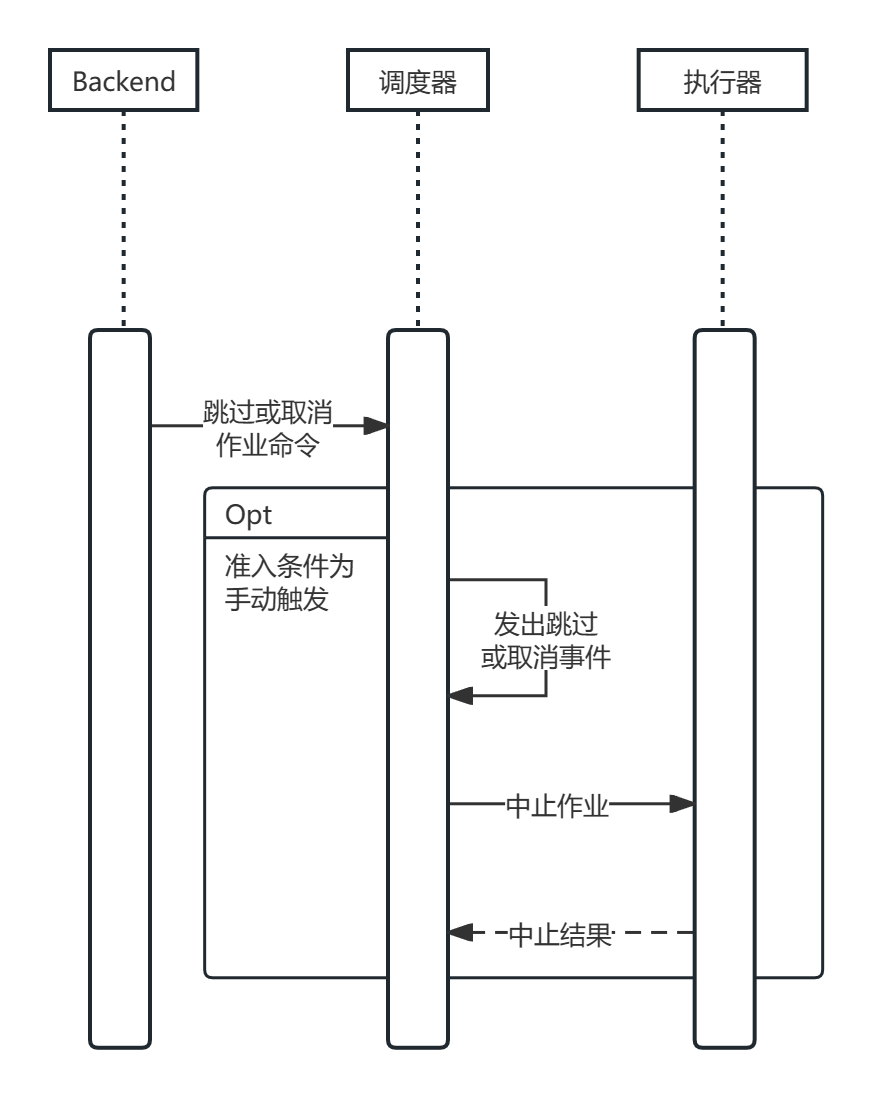
\includegraphics[width=0.8\textwidth]{跳过或取消作业时序图.png}
  \caption{跳过或取消作业时序图时序图}
  \label{fig:跳过或取消作业时序图}
\end{figure}

\paragraph{执行成功与执行失败}
执行失败与执行失败的活动本质上也是类似的,这一事件都是由执行器通知调度器而产生。
当执行器在实际运行环境中检测到作业中任务的脚本执行完毕后,将发送通知调度器的决策中心模块,
同理当执行器在实际允许环境中检测到作业的脚本作业中任务的脚本执行完毕后,将发送任务与整个作业失败的通知给调度器。
决策中心受到通知后,将直接产生执行成功或执行失败的事件,不产生额外的活动,接下来交由调度器进行状态转移。

\subsubsection{作业管理}
该子模块面向Backend对作业进行了二次封装和管理,包括提交作业、获取作业、操作作业,并且接收流水线执行器的作业获取请求和作业执行结果上报,还需要处理作业超时等。

首先,作业管理模块负责将决策中心传来的作业信息进行封装,创建作业实例。每个作业实例包含了执行该作业所需的所有信息,如执行脚本、环境变量和内部各个任务的脚本等。这些信息是执行器执行作业以及后续作业管理的基础。

针对每个作业的执行,作业管理模块都会根据传入的超时时间设定一个超时监控机制。
一旦作业开始执行,计时开始,如果作业执行时间超过了设定的超时时间,作业管理模块将自动触发作业的超时处理活动,中断当前执行的作业,并将触发执行失败事件。
调度器中存在一个检查超时的定时任务,这一定时任务每10秒会检查所有正在执行中的作业,根据作业的开始时间与当前时间计算作业的执行时间,并判断是否超过了预设的超时时间,如果超过了则对超时任务发出执行失败的事件,
同时通知执行器中止作业,避免继续占用资源。
超时处理是确保系统资源不被长时间占用的关键机制,有助于提高系统的整体效率和响应能力。

\subsection{执行器}

执行器的设计目的是为了能够稳定高效地执行不同类型的作业,以待执行的作业信息为输入,以作业执行结果为输出,并且支持快速横向扩展,提高作业执行能力。
作业执行器首先需要能够根据自身能够执行的作业类型获取与之相对应的作业。
获取作业之后,能够保证顺利且高效的完成作业执行。
在执行过程中,将作业内任务的状态上报给调度器;执行完毕后,将作业状态上报给调度器。
执行器本系统将使用开源的Gitlab Runner,GitLab Runner在Gitlab的CI/CD模块中也扮演执行器的功能,并且与Gitlab主模块使用Http Apis进行通信,本系统中将对这些Http Apis进行抓包,获得这些Api的Url以及出入参后,便可如法炮制地将本系统的调度器接入GitLab Runner。
为了保证系统的稳定性,流水线执行器将部署在Kubernetes中,流水线执行器可以根据当前CI/CD的资源需求自动创建或删除副本(在Kubernetes称作Pod),以适应负载的变化:当系统进入使用高峰期时,系统可以自动创建更多的执行器副本来处理请求,而当负载减少时,多余的副本会被自动删除,从而实现资源的高效利用;
同时,当某个执行器发生故障时,Kubernetes会自动检测到故障,并将受影响的CI/CD负载迁移到其他健康的执行器副本上,避免应用程序中断或停止对外提供服务,提高系统稳定性。

\subsection{消息队列}

本系统调度器与执行器之间的消息交互是借助一个消息队列来完成的,本系统中使用阿里巴巴开发的RocketMq 5.0。
当调度器封装好一个流水线作业运行实例时,调度器将作为消息队列的生产者,将作业运行实例放入队列中;执行器作为消息队列的消费者,将持续消费队列中的消息。
调度器和执行器分别与消息队列进行交互,两者之间解耦,便于后续扩展。

系统引入消息队列的主要目的是实现需求分析中的\nameref{subsec:流水线作业合理调度需求}。
首先,消息队列先进先出的特性能够保证执行器有序地消费作业运行实例,避免了程序异步执行带来的作业执行顺序错乱问题,使得作业的执行严格按照调度器预设的顺序执行。
并且,当系统使用高峰期来临,作业量超过了执行器的负载能力时,消息队列承担了缓冲的作用,来不及被消费的作业将按照顺序被堆积在消息队列中,等到执行器处理完当前作业,具备处理能力后,再去消息队列的队头中拉取作业。

调度器、执行器与消息队列之间的时序图如图\ref{fig:消息队列时序图}

\begin{figure}[h]
  \centering
  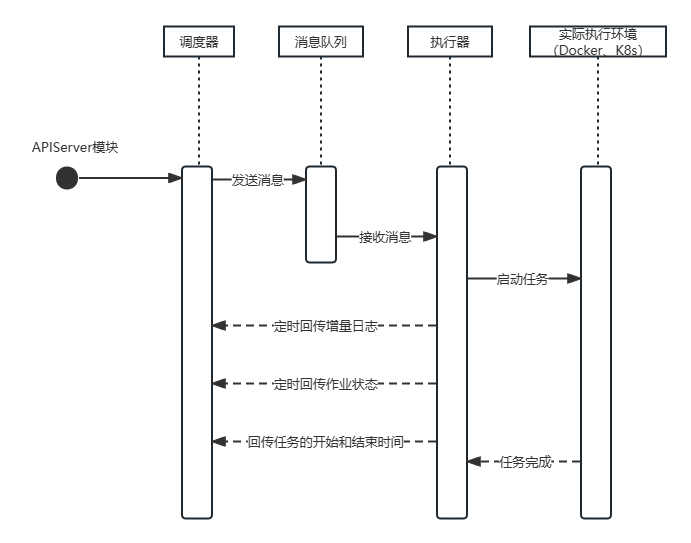
\includegraphics[width=0.8\textwidth]{消息队列时序图.png}
  \caption{调度器、执行器与消息队列间时序图}
  \label{fig:消息队列时序图}
\end{figure}

\subsection{数据存储层}
数据存储层是对本系统中各个数据和文件存储服务的抽象,负责整个系统所有数据的持久化服务。
包括流水线以及其子概念的配置信息、运行记录、Docker镜像、作业执行产物(如编译后压缩产生的tar包等)以及作业运行日志等。


本系统中,使用PostgreSQL存储流水线的配置和运行记录的相关数据,这部分数据属于结构化数据,数据字段和格式较为固定,故采用业界主流的关系型数据库进行存储和管理;
使用Redis存储缓存信息,加快接口的响应速度,提升用户体验;
JFrog Artifactory存储镜像管理模块涉及到的Docker镜像,以及流水线任务执行完成后的执行产物,比如单元测试报告等;
日志平台建立在 Elastic Search 之上,用于集中记录整个系统的所有运行日志,所有子系统的日志都会传送至该平台进行聚合。
其具体原理与功能与本系统主体功能无关,不再赘述。

上述不同类型的数据及其存储方式总结如表\ref{tab:系统数据存储方式}所示.

\begin{table}[h]
  \centering
  \caption{系统数据存储方式}
  \label{tab:系统数据存储方式}
  \begin{tabular}{clll}
    \toprule
    数据类型 & 主要内容      & 存储方式   & 选型 \\
    \midrule
    结构化数据     & 配置信息和运行记录      & 关系型数据库   & PostgreSQL       \\
    缓存数据       & 接口响应数据                   & 键值存储   & Redis       \\
    二进制数据     & Docker镜像、流水线任务执行产物  & 二进制数据管理系统   & JFrog Artifactory   \\
    日志数据       & 日志                & 分布式日志系统  & Elastic Search       \\
    \bottomrule
  \end{tabular}
\end{table}

\section{系统功能设计}

从功能角度,Backend包含以下三个功能模块:流水线管理、镜像管理和节点管理,
其中流水线管理是系统的主体功能,镜像管理以及节点管理服务与流水线作业的环境构建与实际运行。
下文将分别介绍其主要功能设计,系统功能模块图如图~\ref{fig:功能模块图} 所示。

\begin{figure}[h]
  \centering
  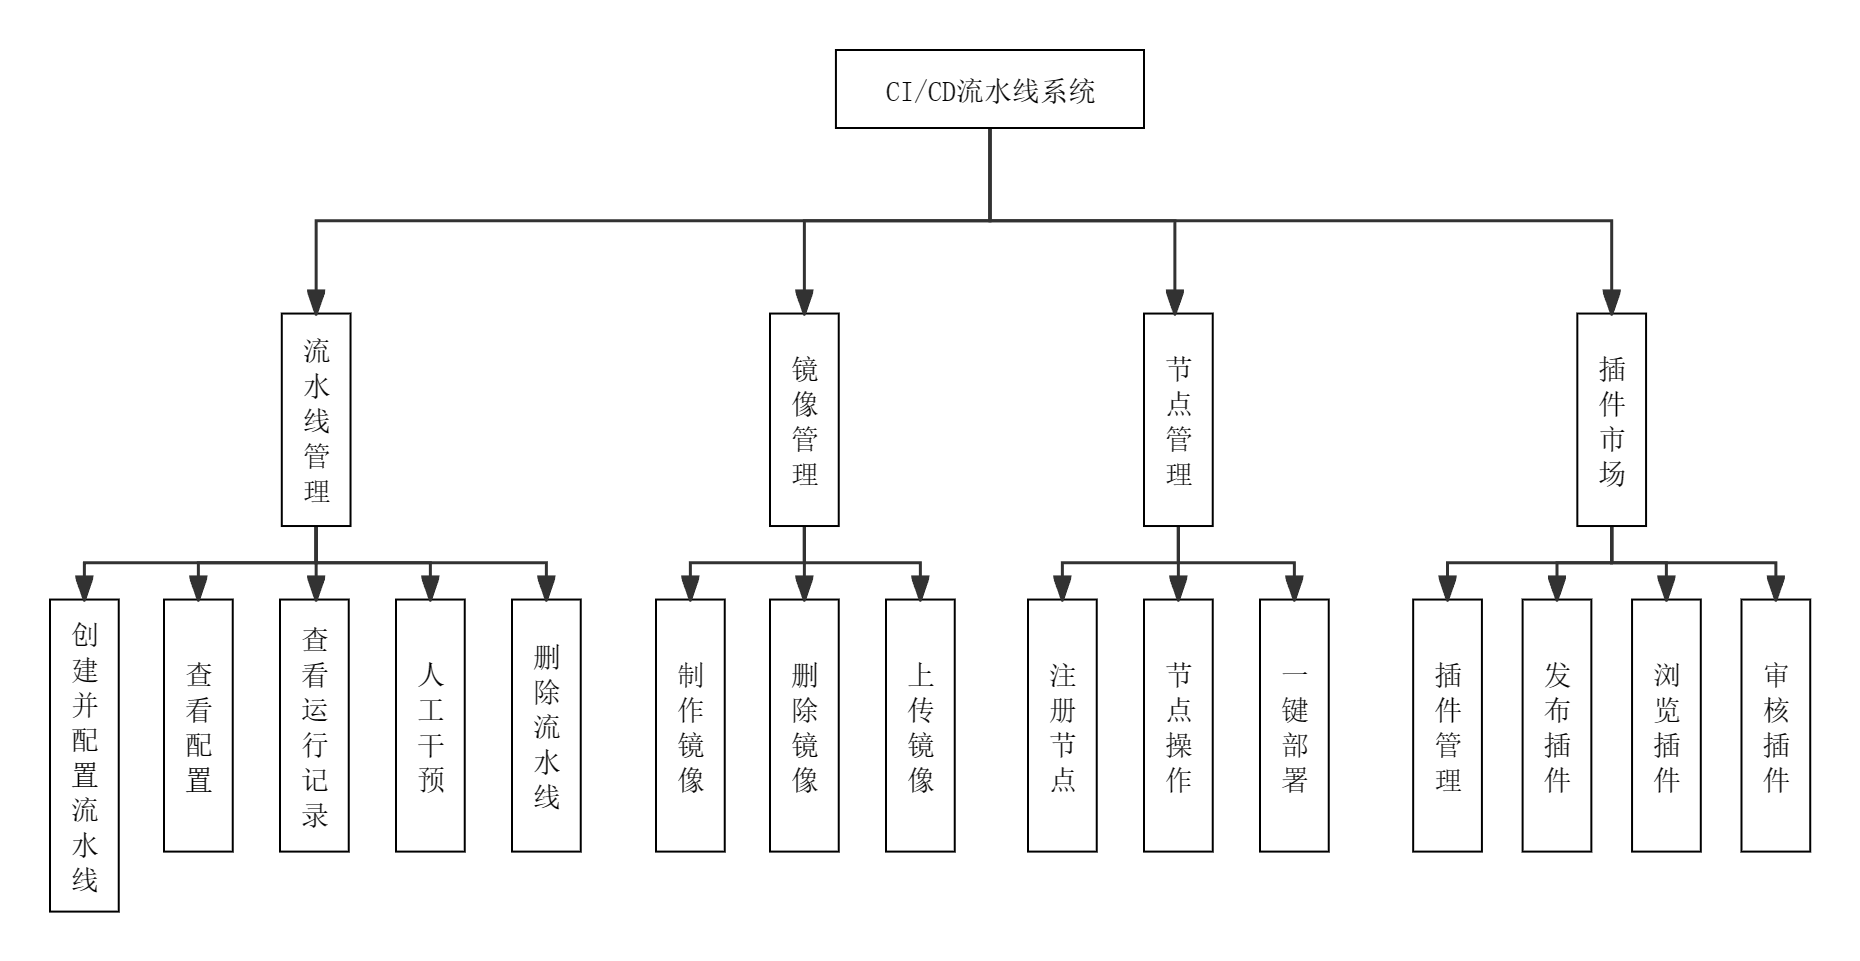
\includegraphics[width=1\textwidth]{功能模块图.png}
  \caption{功能模块图}
  \label{fig:功能模块图}
\end{figure}

\subsection{流水线管理}

流水线管理不仅包括流水线,还包括阶段、作业和任务共四个概念实体,这些实体组成了流水线的拓扑结构。
该模块主要提供了对流水线的基本操作,包括对流水线的增删改查(其中包含了阶段、作业和任务的增删改查)以及流水线的触发。
以下介绍流水线管理中几个关键功能的设计:

\subsubsection{创建并配置流水线}


\subsubsection{触发流水线}


\subsection{镜像管理}
\label{subsec:镜像管理}

在基于容器的CI/CD系统中,镜像是构建容器的基础。
在本系统中,如果用户定义一个作业为容器类型时,首先需要选择一个镜像,作业执行时本系统的执行器会根据镜像来创建环境,然后在环境中执行作业中的各个任务。
为保证系统中的容器可以满足不同开发、测试和运维人员人员的需要,系统中应确保有足够多种类的镜像提供给用户选择,所以镜像管理在本系统中至关重要。

在为了实现镜像管理,系统底层区分并提供了两种主要的服务:一是负责存储镜像的仓库服务,二是负责创建镜像的构建服务。
仓库服务负责对镜像文件进行检索和清除,而构建服务则承担着容器运行和镜像创建的职责。
通过这两类服务的协同工作,实现了高效的镜像管理。

以下介绍镜像管理中几个关键功能的设计:

\subsubsection{镜像创建}

该环节生产的镜像将在创建流水线作业的时候所使用,作为流水线作业的初始环境。
一般来讲,镜像的构建需要管理员直接操作物理服务器,通过手动输入Docker命令来完成,这一过程不仅繁琐而且存在安全风险。
在本系统中,镜像的创建过程被移到了在线平台上,用户可以通过Web界面进行镜像创建。系统支持以下两种方式:
\begin{enumerate}
  \item 通过DockerFile文件。这是最常见的构建镜像的方法,用户需要在系统中按照特定语法编写DockerFile,其中可以指定基础镜像、构建命令、端口暴露、文件挂载等。
  这要求用户对DockerFile的编写的语法规则以及shell脚本有所了解。
  \item 通过Commit操作。该方法允许将运行中的容器状态保存为新镜像,此过程中需要基于一个初始镜像启动容器,然后进行环境配置,最终提交更改为新镜像。
\end{enumerate}

这两种方法提供了不同的优势和选择灵活性。其中通过Commit操作的方式需要在用户界面中远程连接到容器,这需要借助基于网页的SSH组件(如Wetty、Guacamole、GateWay等)实现,
本系统中使用Wetty实现用户在Web端与容器内部的交互。

当用户制作镜像时,首先需要填写镜像基础信息,如镜像名、标签等,然后Backend模块会检查数据库中是否有冲突的镜像,如果有则重新返回上一步进行填写。
接下来需要用户选择制作方式,如果用户选择Dockerfile方式,则可以在线编写Dockerfile文件或者直接上传文件,然后镜像制作服务器将调用docker build命令来构建镜像,并返回镜像构建结果;
如果用户选择commit方式,则需要用户选择一个基础镜像,镜像服务器将根据基础镜像调用docker run启动一个容器实例,并暴露出SSH服务的端口,用户在前端通过Wetty进入容器后,进行一系列操作后,
服务器中将调用docker commit将该容器提交为镜像。

镜像制作的活动图如图~\ref{fig:镜像制作活动图}所示。

\begin{figure}[h]
  \centering
  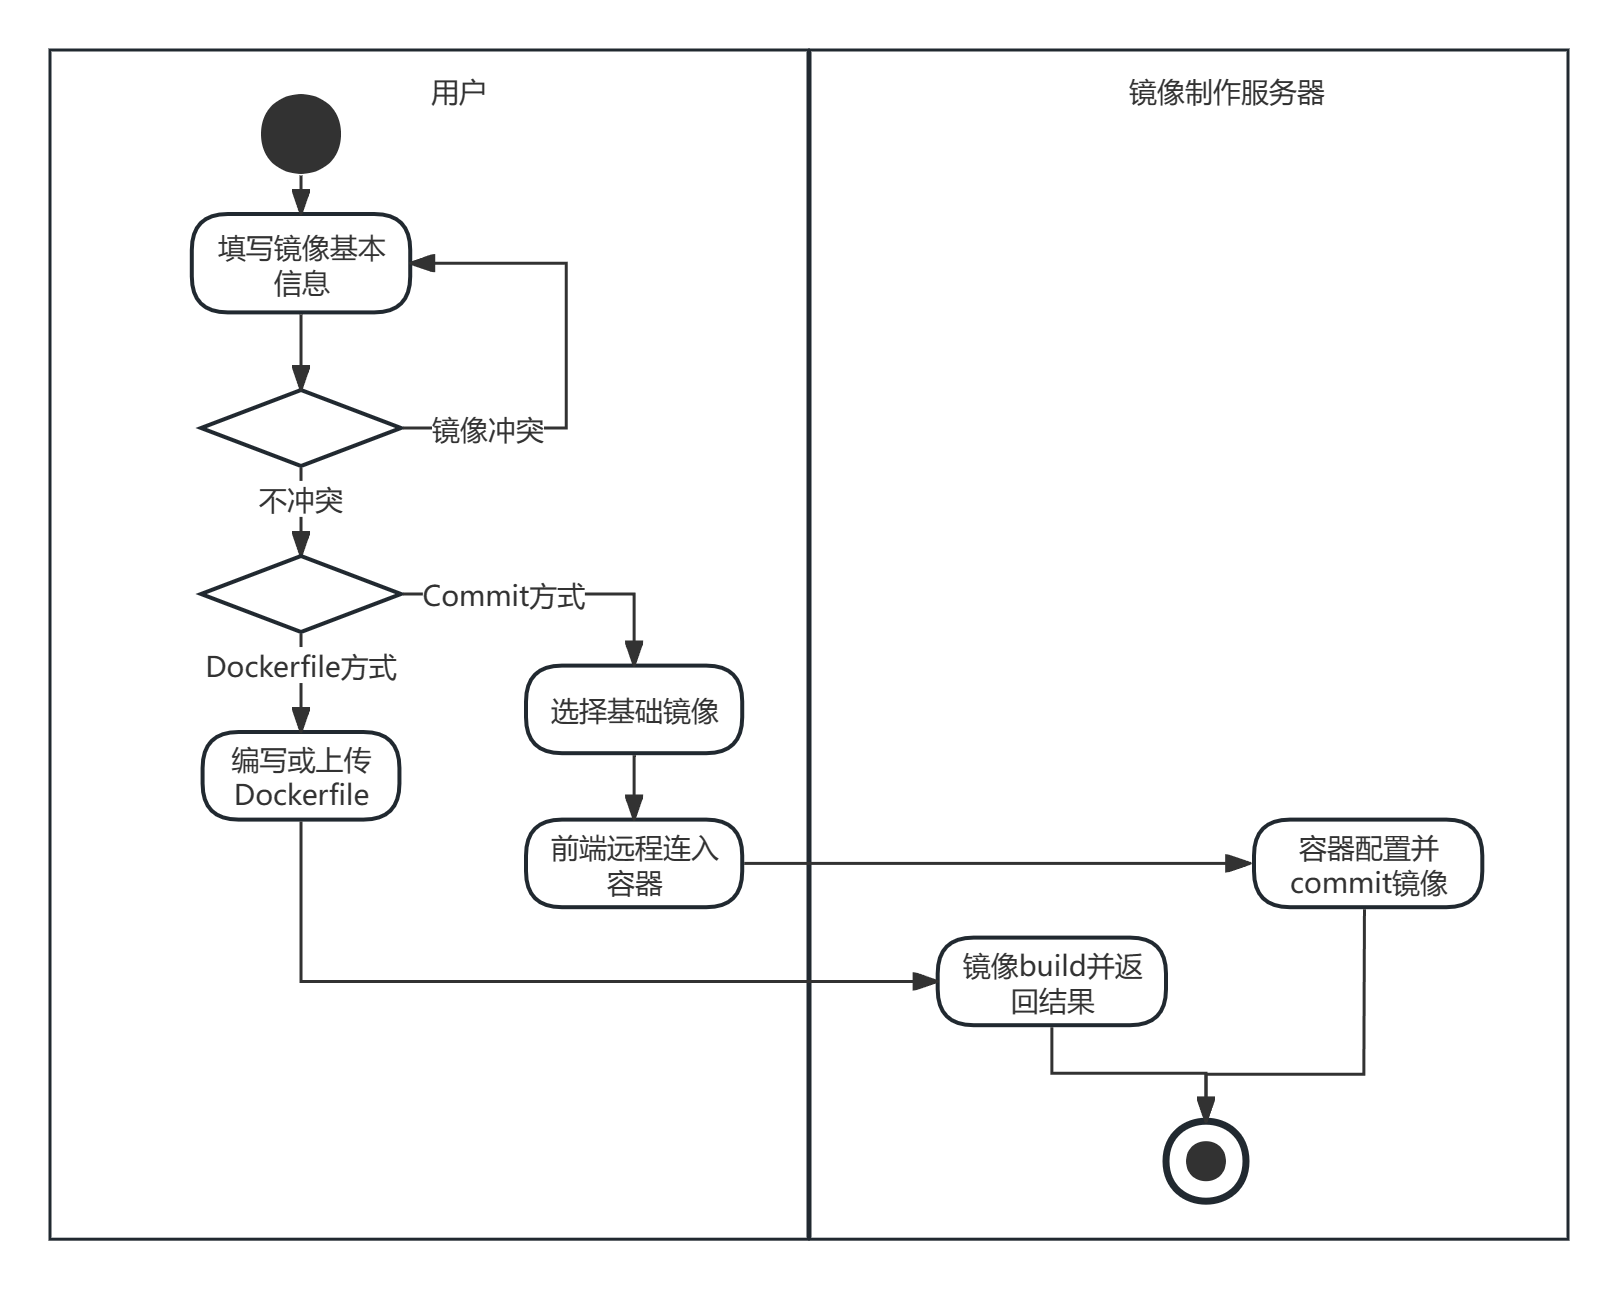
\includegraphics[width=1\textwidth]{镜像制作活动图.png}
  \caption{镜像制作活动图}
  \label{fig:镜像制作活动图}
\end{figure}

\subsubsection{镜像删除}

由于系统中需要支持多样的流水线作业,也就势必需要各种各样的镜像。
随着镜像数量的增加,镜像仓库的存储压力也随之上升,因此需要及时清理不再需要的镜像。

尽管Docker官方提供了删除镜像的API,但该API无法清除所有相关文件。
Docker镜像为了节省存储和带宽,采用了分层构建的机制,镜像的每一层都是基于上一层的更改或添加,每一层都是一个单独的文件。
当一个镜像被推送到系统的镜像仓库,每个镜像会拥有一个Manifest文件,这个文件记录了所有组成本镜像所需要的层。
而当调用Docker API删除一个镜像时,只是删除了镜像所对应的Manifest文件,并不会删除其引用的层,这样就导致有些没有被引用的层残留在仓库中。

如图~ \ref{fig:镜像-Manifest文件-层级关系图}所示,有两个镜像分别对应两个Manifest文件,其中Manifest1引用layer1、layer2、layer3,Manifest1引用layer3和layer4。
当我们调用Docker API删除镜像1后,实际上仓库中被删除的只是Manifest1文件,而此时layer4已经不被任何Manifest文件所引用,但却没有被真正删除。

\begin{figure}[h]
  \centering
  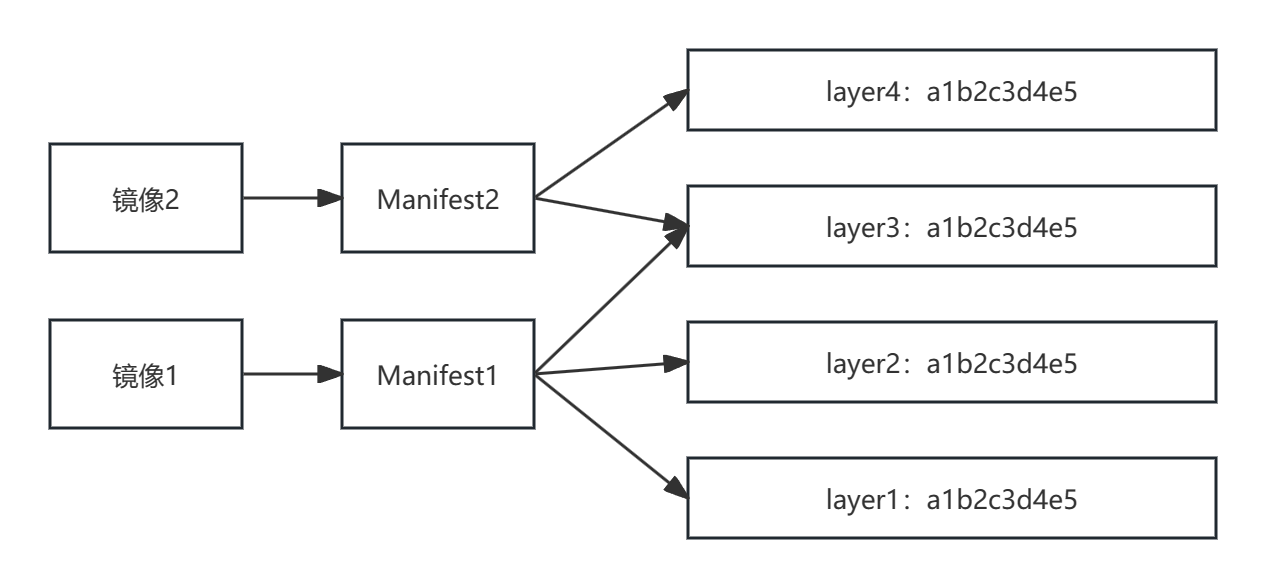
\includegraphics[width=1\textwidth]{镜像层级图.png}
  \caption{镜像-Manifest文件-层级关系图}
  \label{fig:镜像-Manifest文件-层级关系图}
\end{figure}

为解决这一问题,系统中引入了引用计数的功能,这一思想在软件工程中经常被运用,如智能指针、垃圾回收等。
系统将为每一个layer维护其引用计数,当某一层的引用次数降至零时,相应的物理文件也会被删除,从而真正释放存储空间。

镜像删除的活动图如图~\ref{fig:镜像删除活动图}所示。

\begin{figure}[h]
  \centering
  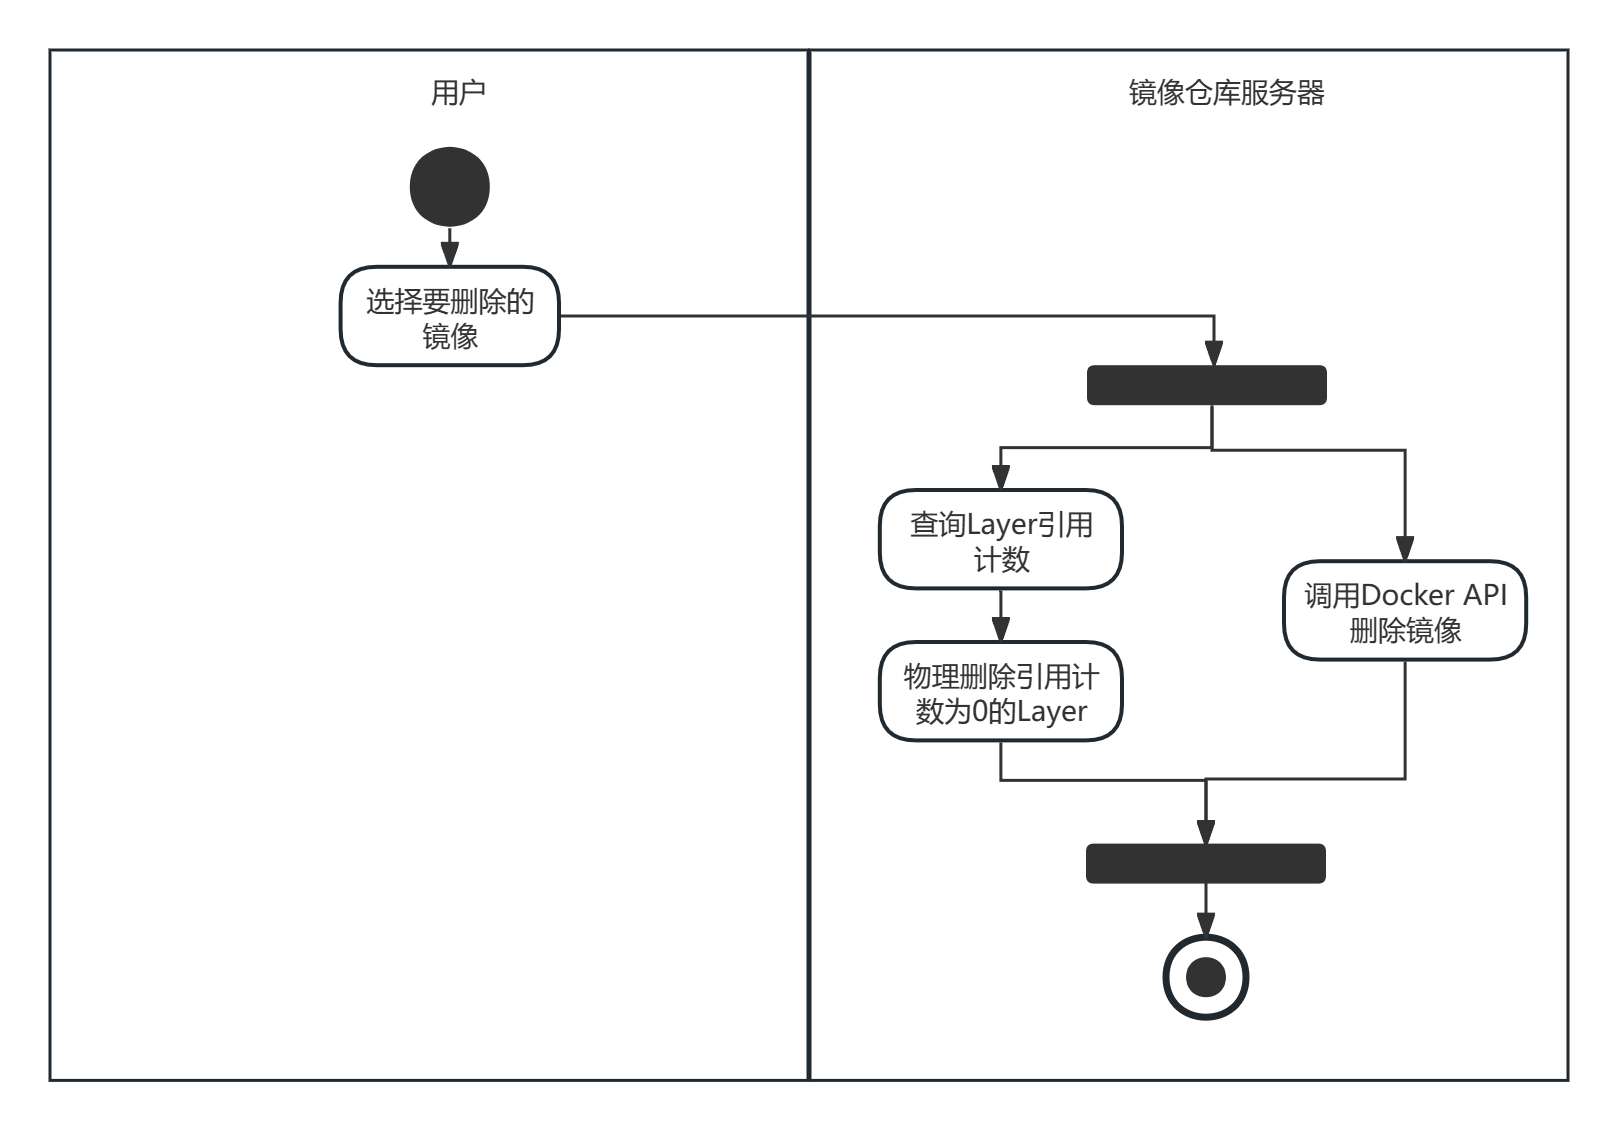
\includegraphics[width=1\textwidth]{镜像删除活动图.png}
  \caption{镜像删除活动图}
  \label{fig:镜像删除活动图}
\end{figure}

\subsubsection{镜像上传}
镜像上传功能使用户能够将创建好的镜像推送至仓库中保存。
考虑到镜像移除功能的改进,上传过程中也需要对层引用记录进行相应的更新,以保持系统数据的一致性和完整性。

在上传镜像时,制作服务器调用Docker API推送镜像至仓库。
镜像制作服务器随后通知仓库服务器更新层引用记录文件。
仓库服务器在接收到更新请求后,检查记录文件状态,并据此更新层引用计数。

\subsection{节点管理}
在CI/CD流水线系统中,执行器负责流水线作业的执行,为了满足执行器执行所需的作业的物理与系统环境,执行器所部署的服务器也应有所不同。
节点的本质就是一台物理机或虚拟机,系统使得用户可以自主地对节点进行部署、上下线和删除,以便根据自身作业的需要为其配置所需环境,
对于节点的管理往往同时涉及到数据库节点记录的管理以及对服务器的操作。

\subsubsection{节点注册}
节点注册是系统中对新加入节点进行识别和管理的初步过程。
在设计上,节点注册流程首先需要节点通过调用系统API或通过用户界面手动注册,提交节点的基本信息,如名称、类型(如物理机、虚拟机或Docker)、IP地址、主机名以及任何特定的标签。
这些信息被用于创建节点的唯一标识符(UUID),确保在系统中每个节点都具有唯一性。

注册过程中,系统会校验提交的信息,包括IP地址的格式和可达性、主机名的有效性以及凭证的正确性。
注册成功后,节点的状态被设置为“待部署”,等待后续的一键部署过程完成。
此外,注册流程还包括标签(Tag)管理,一个节点应指定一个或多个标签,这个Tag与创建流水线作业时所指定的Tag是一一对应的,节点中的执行器只会从消息队列中拉取Tag相同的作业进行执行。

\subsubsection{节点一键部署}

节点的一键部署是提升系统效能的关键功能,省去了用户自己去服务器进行执行器部署的步骤。
首先,系统会根据用户提供的IP和部署凭证(用户名、密钥或密码)建立SSH连接,然后创建远程目录,以确保存储配置文件和二进制文件的目录存在,
在此之后备份目标服务器上现有的配置文件,创建或打开新的配置文件和系统ID文件,准备写入新的配置,到此为止,节点部署的准备工作完成。
下载并设置执行器的二进制文件,根据提供的配置,生成执行器的配置文件(config.toml)和系统ID文件,编写并配置执行器的systemd服务文件,以便在系统启动时自动启动执行器。
创建或更新/nix目录,并设置为NFS挂载点(如果需要)。通过systemd管理执行器服务:重新加载systemd守护进程,启用并启动执行器服务,最后关闭SSH连接以释放资源。
如果一切顺利,在执行器成功部署后,该服务器便成为了系统中的一个节点,能够与系统主体进行通信并在该节点上执行流水线作业。

节点一键部署活动图如图~ \ref{fig:节点一键部署活动图}所示。

\begin{figure}[h]
  \centering
  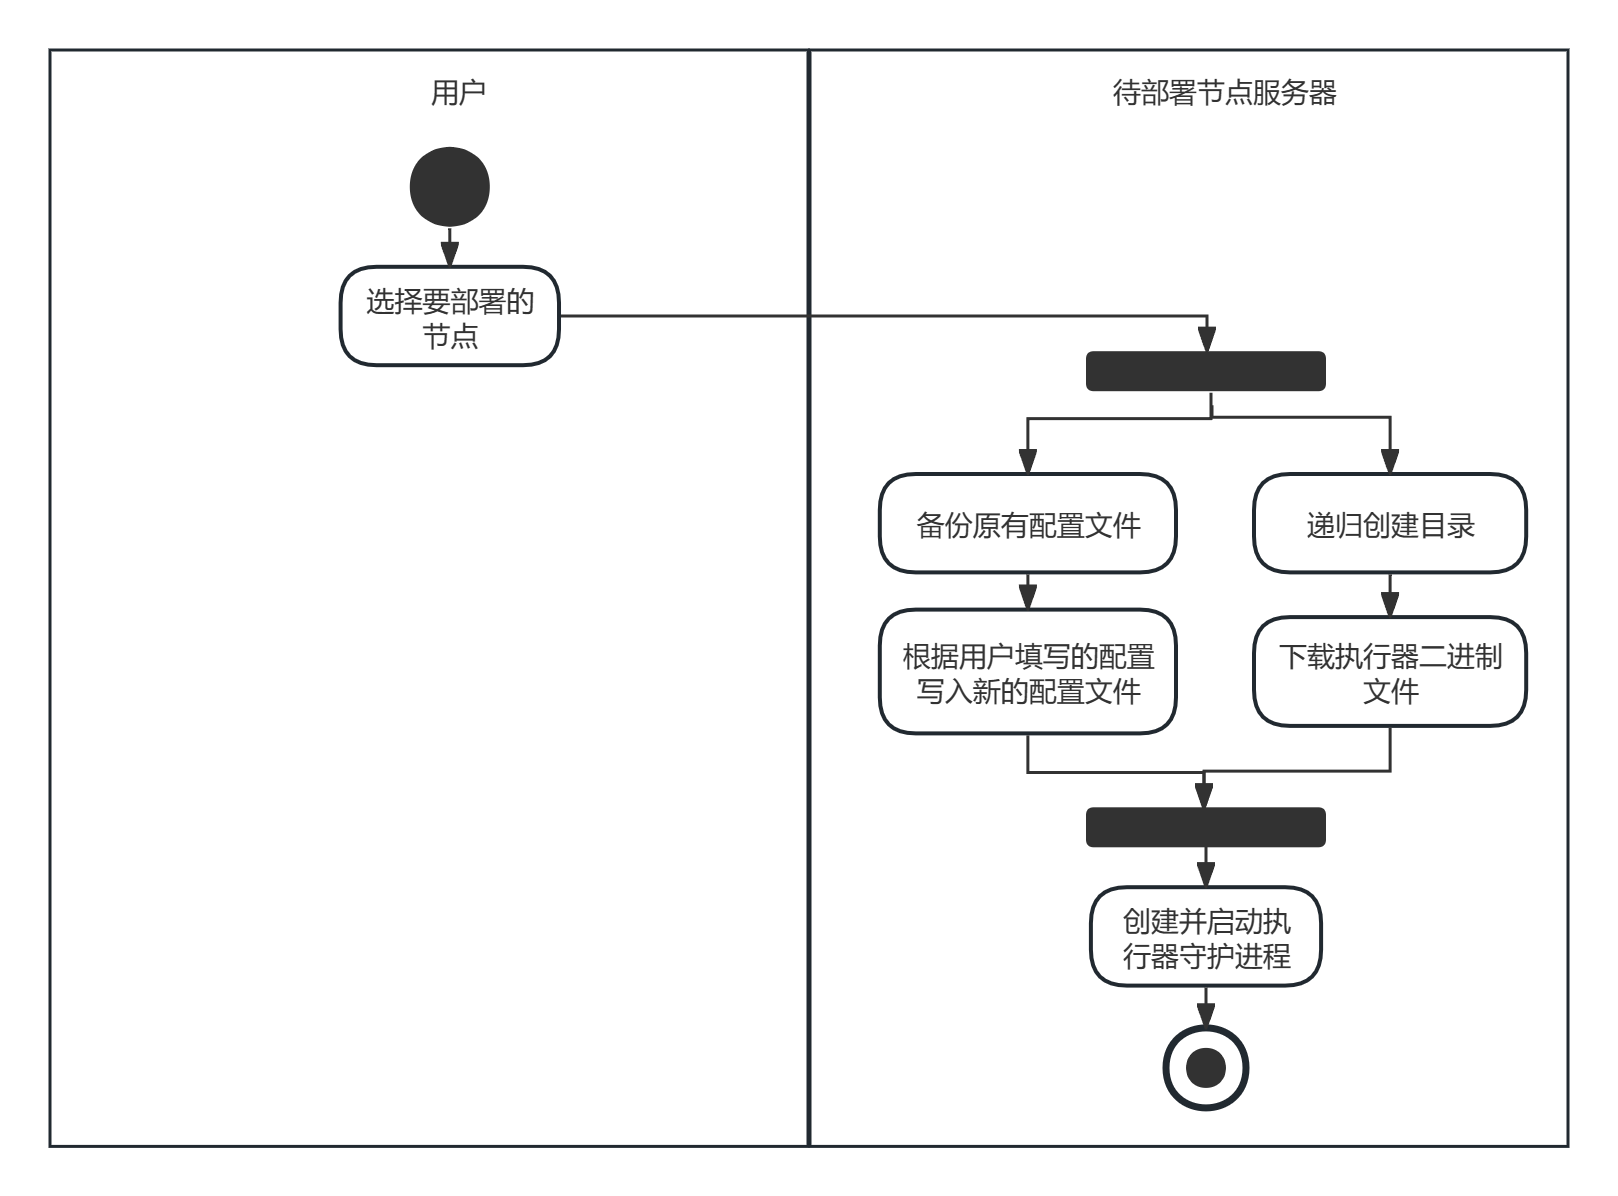
\includegraphics[width=1\textwidth]{节点一键部署活动图.png}
  \caption{节点一键部署活动图}
  \label{fig:节点一键部署活动图}
\end{figure}

\subsubsection{节点的上线与下线}
与一键部署同理,在节点的上线与下线过程中,不仅需要在调度系统中更新节点状态,还需要在部署节点的服务器上执行具体的操作以确保这一状态变化得以实际反映。

对于节点上线来说,首先需要SSH连接到节点服务器,使用systemctl start命令启动节点注册时配置好的执行器服务。
此后需要进行必要的健康检查,包括验证服务进程的状态、测试服务与消息队列和调度器的网络连通性等,
因为节点对应服务器的文件内容和网络状态在节点未上线的过程中,可能会受到其他用户的修改,所以健康检查是确保节点能够成功接收和执行作业,保证节点正常运作的必要步骤。

节点上线的活动图如图\ref{fig:节点上线活动图}所示。

\begin{figure}[h]
  \centering
  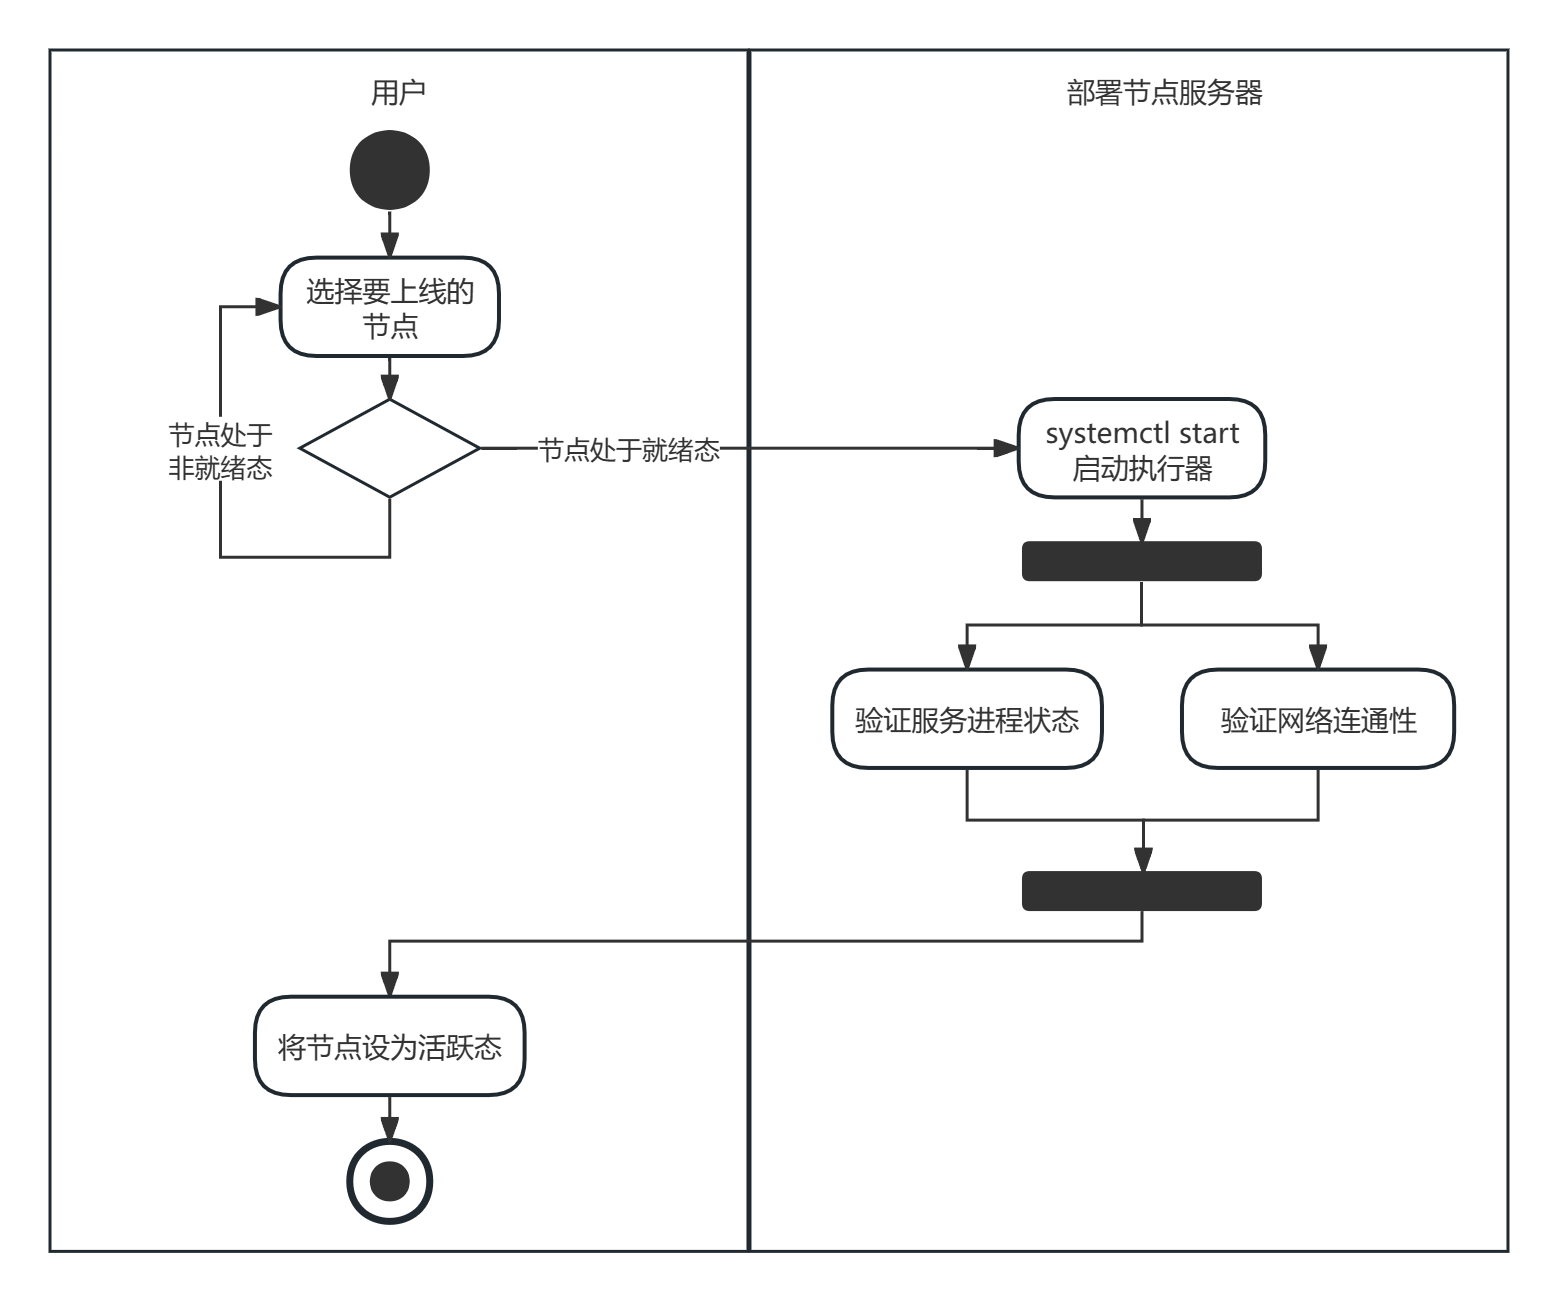
\includegraphics[width=1\textwidth]{节点上线活动图.png}
  \caption{节点上线活动图}
  \label{fig:节点上线活动图}
\end{figure}

对于节点下线来说,首先需要安全地停止服务器中的执行器服务,这时如果节点中仍然有执行中的任务,节点将对当前作业进行保持,并将节点设置为待下线的状态,
设置这一状态主要是为了与在线状态进行区分,避免执行完当前任务后又从消息队列中拉取下一任务,导致一直无法下线节点。
待当前作业结束后,进行后处理步骤,首先使用systemctl stop命令停止服务,然后执行必要的清理操作,如临时文件清理和日志上传等,以保证节点下次上线时处于清洁状态,同时减少对相应服务器的磁盘占用。
以上步骤均成功后,节点将被设置为离线状态。

节点下线的活动图如图\ref{fig:节点下线活动图}所示。

\begin{figure}[h]
  \centering
  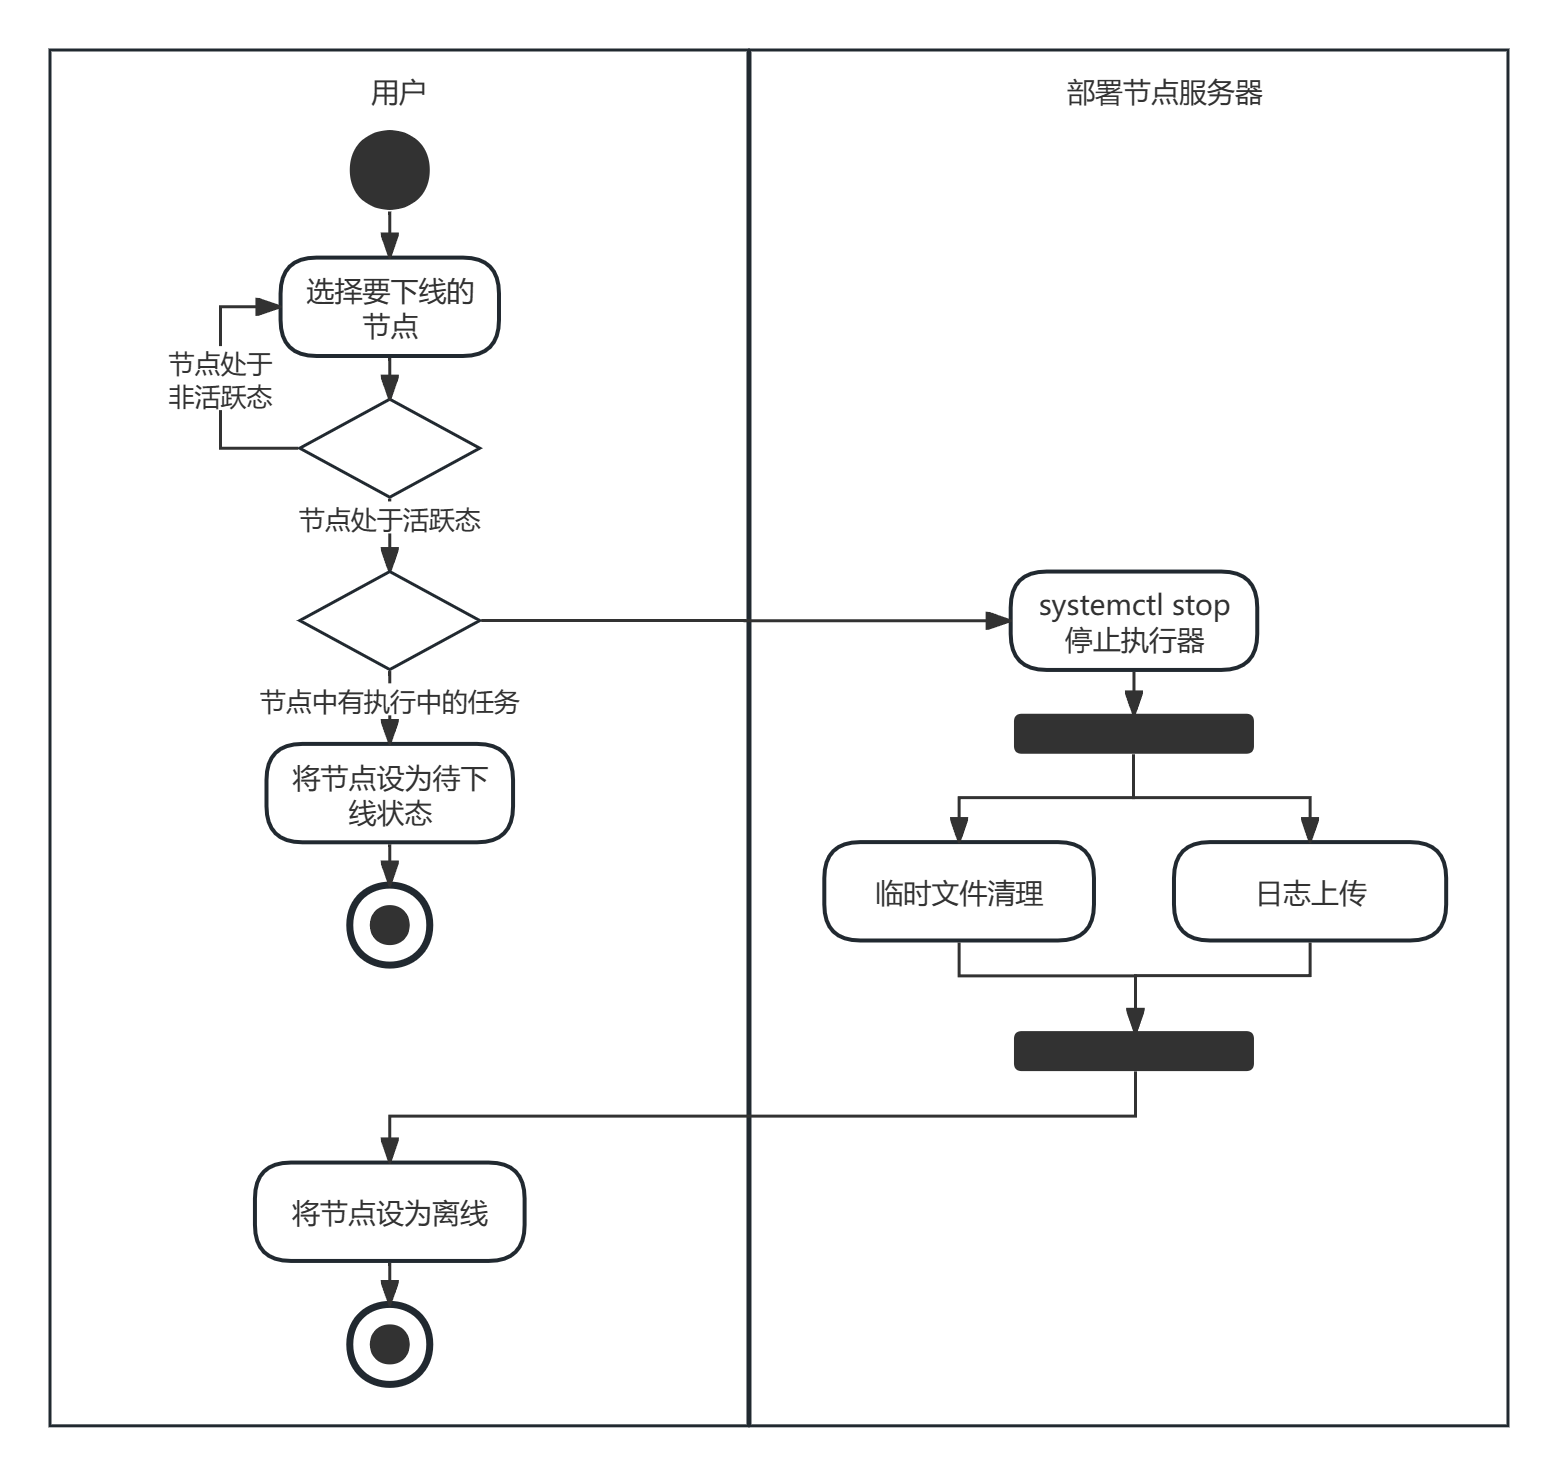
\includegraphics[width=1\textwidth]{节点下线活动图.png}
  \caption{节点下线活动图}
  \label{fig:节点下线活动图}
\end{figure}

\subsubsection{节点删除}
节点删除功能允许管理员从系统中彻底移除不再需要的节点,包括数据库记录和部署在服务器上的执行器服务。
删除节点时,首先需要检查节点的状态,如果节点是未部署的状态,直接由Backend模块删除节点的记录即可。
如果是在线或者待下线的状态,则会提示用户无法删除。
如果是离线状态,系统则需要在删除记录的同时,SSH进入服务器中调用执行器的卸载脚本,递归删除执行器的目录。

节点删除的活动图如图\ref{fig:节点删除活动图}所示。

\begin{figure}[h]
  \centering
  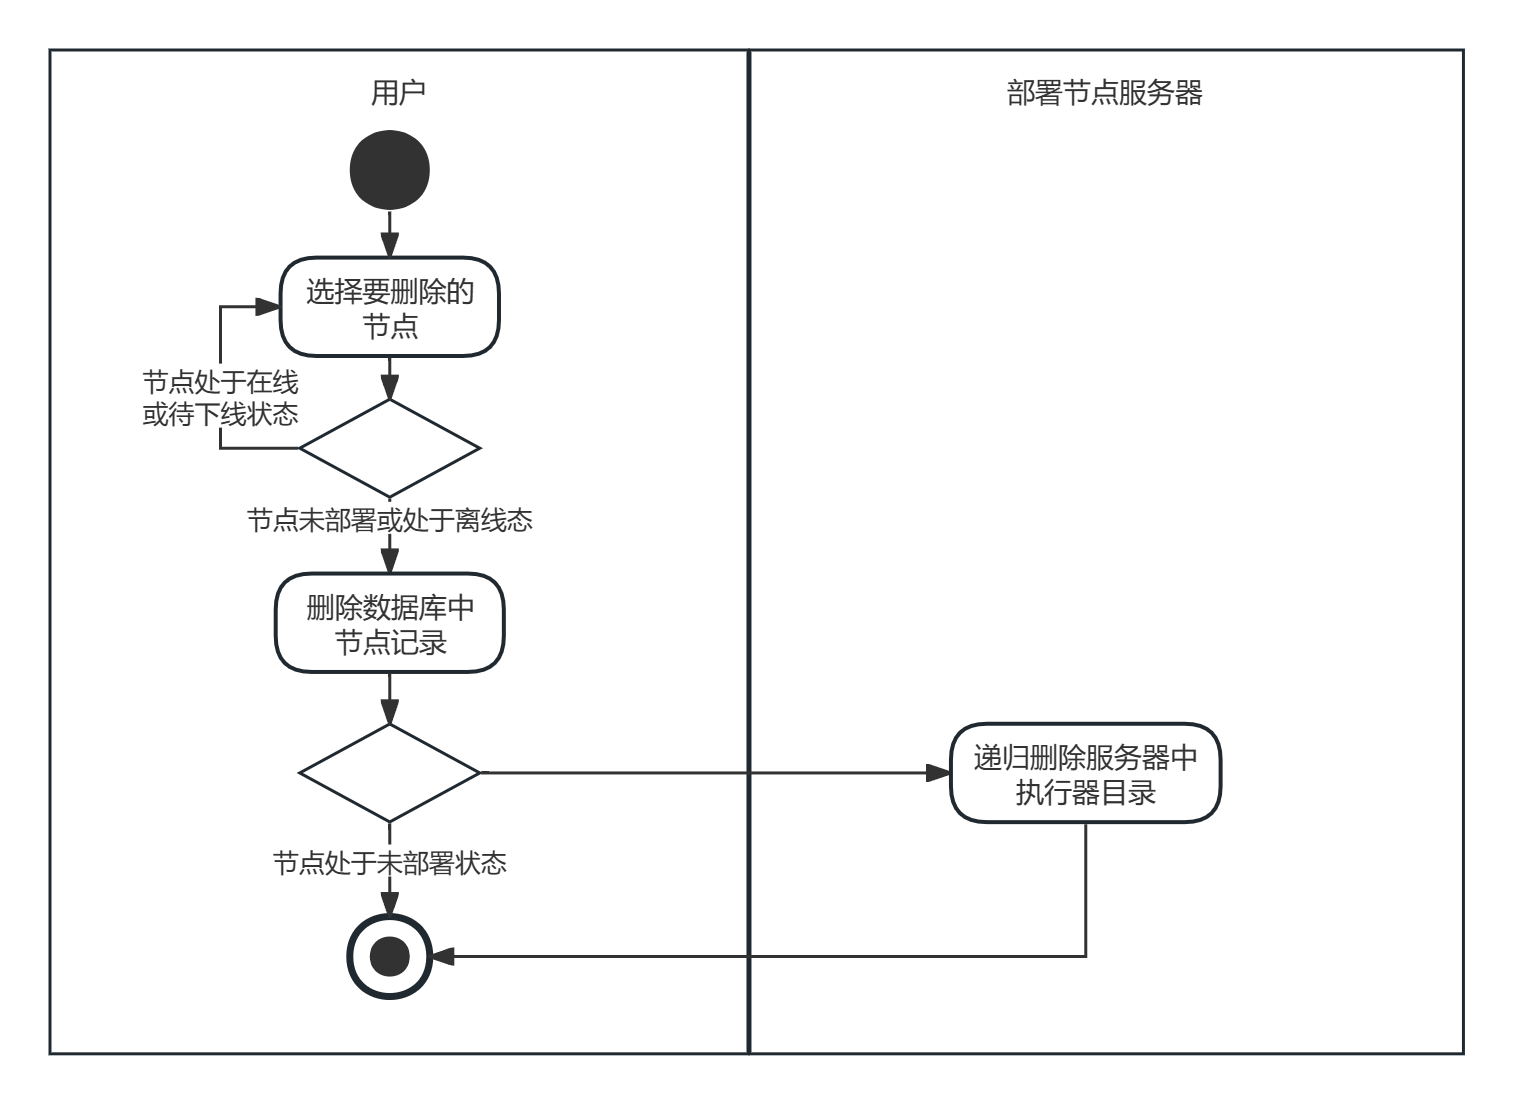
\includegraphics[width=1\textwidth]{节点删除活动图.png}
  \caption{节点删除活动图}
  \label{fig:节点删除活动图}
\end{figure}

\section{数据模型设计}
这一部分将系统中的数据进行抽象,从实体、属性和关系三个维度设计出系统的数据模型,并基于此完成了对数据表的设计。

本系统中的与流水线相关的数据实体可以分为两类,一种是配置(Config)相关实体,一种是运行(RunInfo)相关实体。
同时,由于流水线中存在四个不同层级的子概念,所以本系统中可梳理出2×4=8个与流水线相关的实体:
流水线配置、阶段配置、作业配置、任务配置、流水线运行记录、阶段运行记录、作业运行记录、任务运行记录。

同时,根据前文对需求的整理和分析,系统中还需要对镜像、节点和插件三个概念进行抽象,而节点又是根据Tag标签的方式与作业进行联系的。
所以系统中还应有镜像、节点、节点标签和插件四个实体,加上流水线相关实体,共12个实体。

接下来对实体中的主要属性进行分析,由于流水线相关实体较多且内容具有相似性,此处选取代表性的“作业”相关实体进行分析。

对于作业配置相关实体,应主要包含以下几个方面的属性:
基本信息类包括作业id(主键)、作业所属的阶段id(外键)、名称、创建时间、修改时间、作业位于阶段中的位置;
构建信息类包括,包括 Docker 镜像、输入环境变量;
执行信息类包括:超时时间、触发类型(自动/人工/定时)、是否启用。
可以得到数据库中作业配置表如表~ \ref{tab:作业配置表}

\begin{table}[h]
  \centering
  \caption{作业配置表}
  \label{tab:作业配置表}
  \begin{tabular}{cll}
    \toprule
    字段名                  & 类型            & 描述                                       \\
    \midrule
    id                      & Char           & 主键id                                   \\
    name                    & Char           & 作业名称                                   \\
    trigger\_type           & Char           & 触发方式,自动/手动                        \\
    stage\_config\_id       & ForeignKey     & 关联的阶段配置                             \\
    created\_at             & DateTime       & 创建时间                                    \\
    updated\_at             & DateTime       & 更新时间                                    \\
    image\_id               & ForeignKey     & 关联的Docker镜像                            \\
    variables               & JSON           & 未赋值环境变量                              \\
    tag                     & Char           & 标签                                       \\
    timeout                 & Integer        & 超时时间                                    \\
    position                & Integer        & 位置                                        \\
    run\_condition          & Char           & job的运行条件                               \\
    active                  & Boolean        & 是否启用                                    \\
    version                 & Integer        & 版本号,以追溯修改历史                        \\
    \bottomrule
  \end{tabular}
\end{table}

对于运行记录相关实体,以作业运行记录为例,应包含以下几个方面的属性:
基本信息类包括作业运行记录id(主键)、作业运行记录所属的阶段运行记录id(外键)、作业运行记录所属的作业id(外键);
触发信息类:触发时间、触发人、触发类型;
运行信息类:开始时间、结束时间、作业状态、赋值后的环境变量;
可以得到数据库中作业运行记录表如表~ \ref{tab:作业运行记录表} 所示。

\begin{table}[h]
  \centering
  \caption{作业运行记录表}
  \label{tab:作业运行记录表}
  \begin{tabular}{cll}
    \toprule
    字段名               & 类型          & 描述                                               \\
    \midrule
    job\_config\_id     & ForeignKey   & 关联的作业配置                                     \\
    stage\_run\_info\_id    & ForeignKey   & 关联的阶段运行信息                                 \\
    started\_at         & DateTime     & 作业运行开始时间                                   \\
    end\_at             & DateTime     & 作业运行结束时间                                   \\
    repo\_url           & Char         & 代码仓库URL                                      \\
    repo\_branch        & Char         & 分支名                                           \\
    ref\_sha            & Char         & commit id                                       \\
    variables           & JSON         & 赋值后的环境变量                                  \\
    state               & Char         & 作业的状态,如pending/running/success等            \\
    selected            & Boolean      & 触发时是否勾选,布尔值                             \\
    \bottomrule
  \end{tabular}
\end{table}

其余的流水线配置、阶段配置与任务配置中的属性与作业配置大同小异,此处不再赘述。

然后分析镜像、节点、节点标签和插件四个实体。
对于Docker镜像,有镜像名、镜像ID、镜像描述等基本信息,同时应有镜像标签(Image Label)镜像地址等与镜像存储相关的属性;
节点的本质是一个服务器,应包含服务器信息,如服务器IP、端口号、主机名、登录凭证等,同时也应包含节点名称、节点描述等基本信息。
节点标签是不同作业分配到不同节点上的依据,同时又是节点与作业多对多关系的中间表,包含名称、节点ID、作业ID等属性;
插件作为任务的模板,包含了大部分任务实体中的属性,如脚本内容、环境变量等,同时包含一些插件特有的属性,如版本号、配置表单、插件logo等。

最后分析系统内实体之间的关系。一个配置的一次执行即产生了一个运行实例,这与编程语言中“类”和“类对象”的关系类似,
即“运行”是“配置”的实例化,“配置”是“运行”的模板,因此配置与运行是一对多的关系。
同时根据流水线的各个子概念的定义,我们知道有:流水线与阶段是一对多的关系,阶段与作业是一对多的关系,作业与任务是一对多的关系。
由于作业中包含镜像,所以镜像与作业是一对多的关系。
每个作业需要指定一个节点或多个节点,每个节点又可以被多个作业所指定,所以作业与节点是多对多的关系,作业标签自然就是作业与节点的中间表。
插件由于是任务的模板,所以与任务是一对多的关系,一个插件可以应用于多个任务,一个任务只能指定一个插件。

结合以上分析,可得出系统的实体-关系图(E-R图)如图~\ref{fig:系统E-R图}:

\begin{figure}[h]
  \centering
  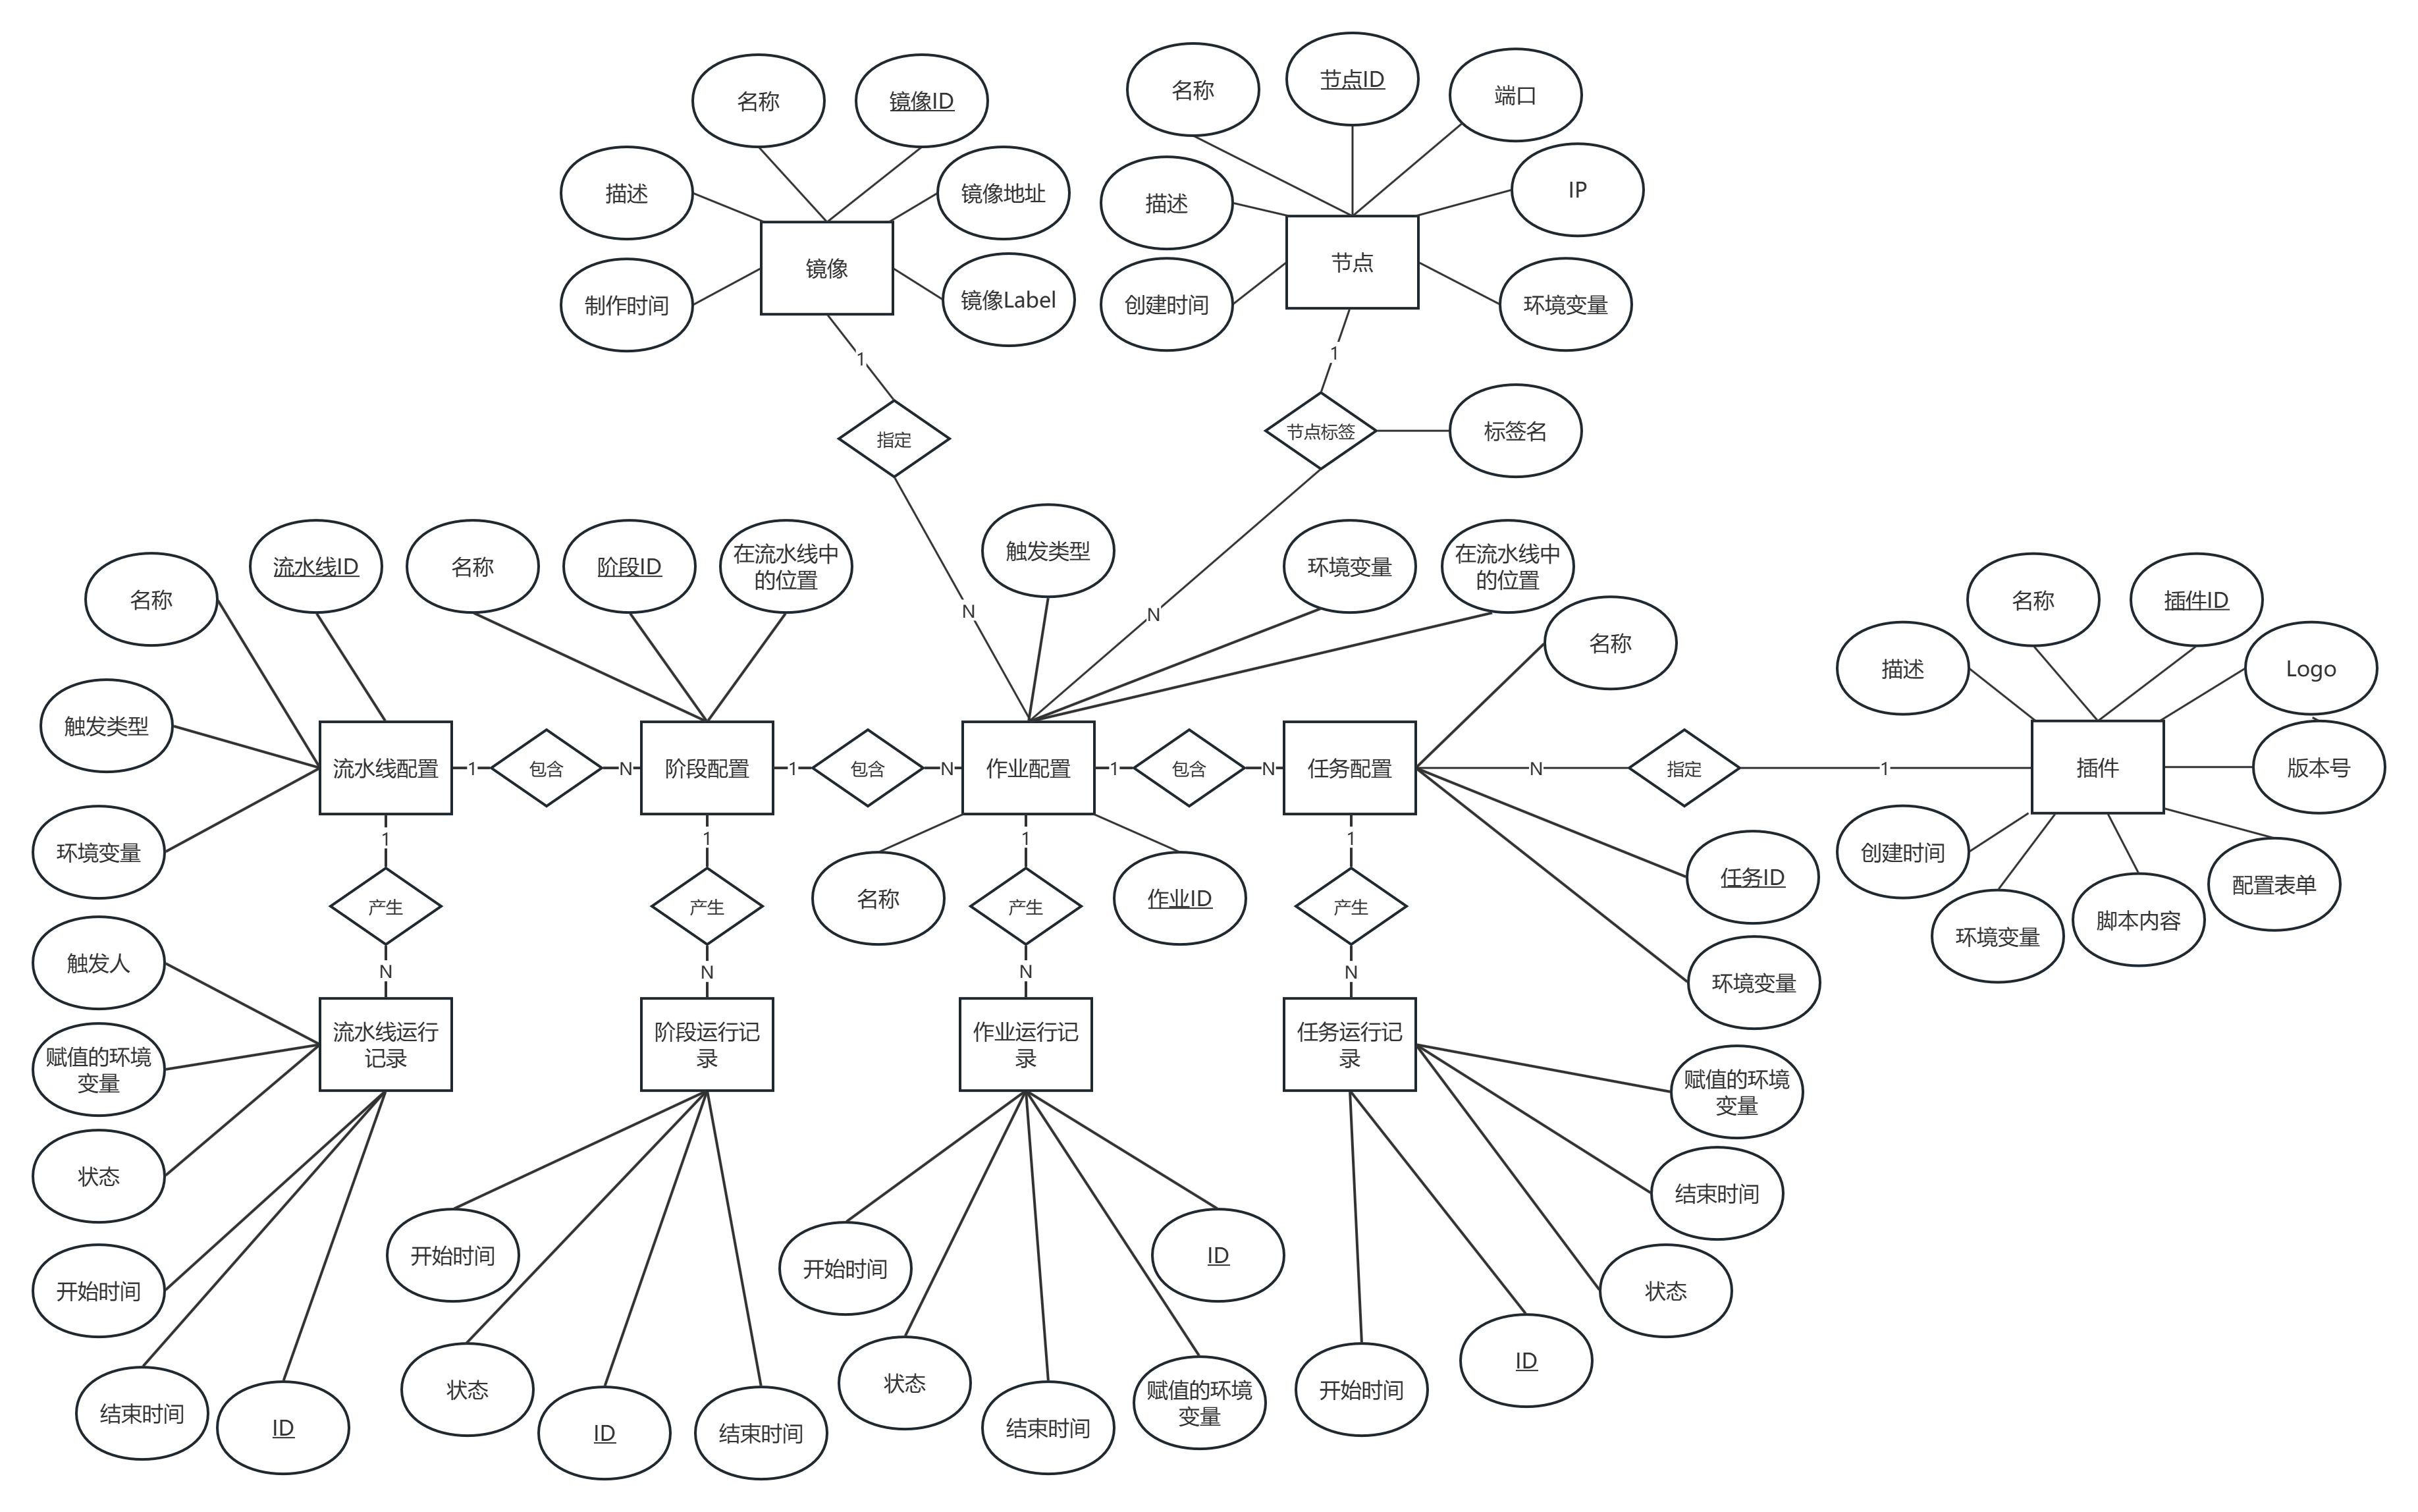
\includegraphics[width=1\textwidth]{系统ER图.png}
  \caption{系统E-R图}
  \label{fig:系统E-R图}
\end{figure}



% !TeX root = ../main.tex

\chapter{系统详细设计与实现}
本章将从具体的细节上着手阐述系统中各个功能模块与架构模块的具体实现,重点在于内部算法和数据结构的设计与实现。

\section{流水线管理}
流水线管理主要包含对流水线中各个子概念及其操作的封装,包括流水线实体类、流水线运行记录类、阶段实体类、阶段运行记录类、作业实体类、作业运行记录类、任务实体类、任务运行记录类。
类图如图\ref{fig:流水线管理类图}所示。
\begin{figure}[h]
  \centering
  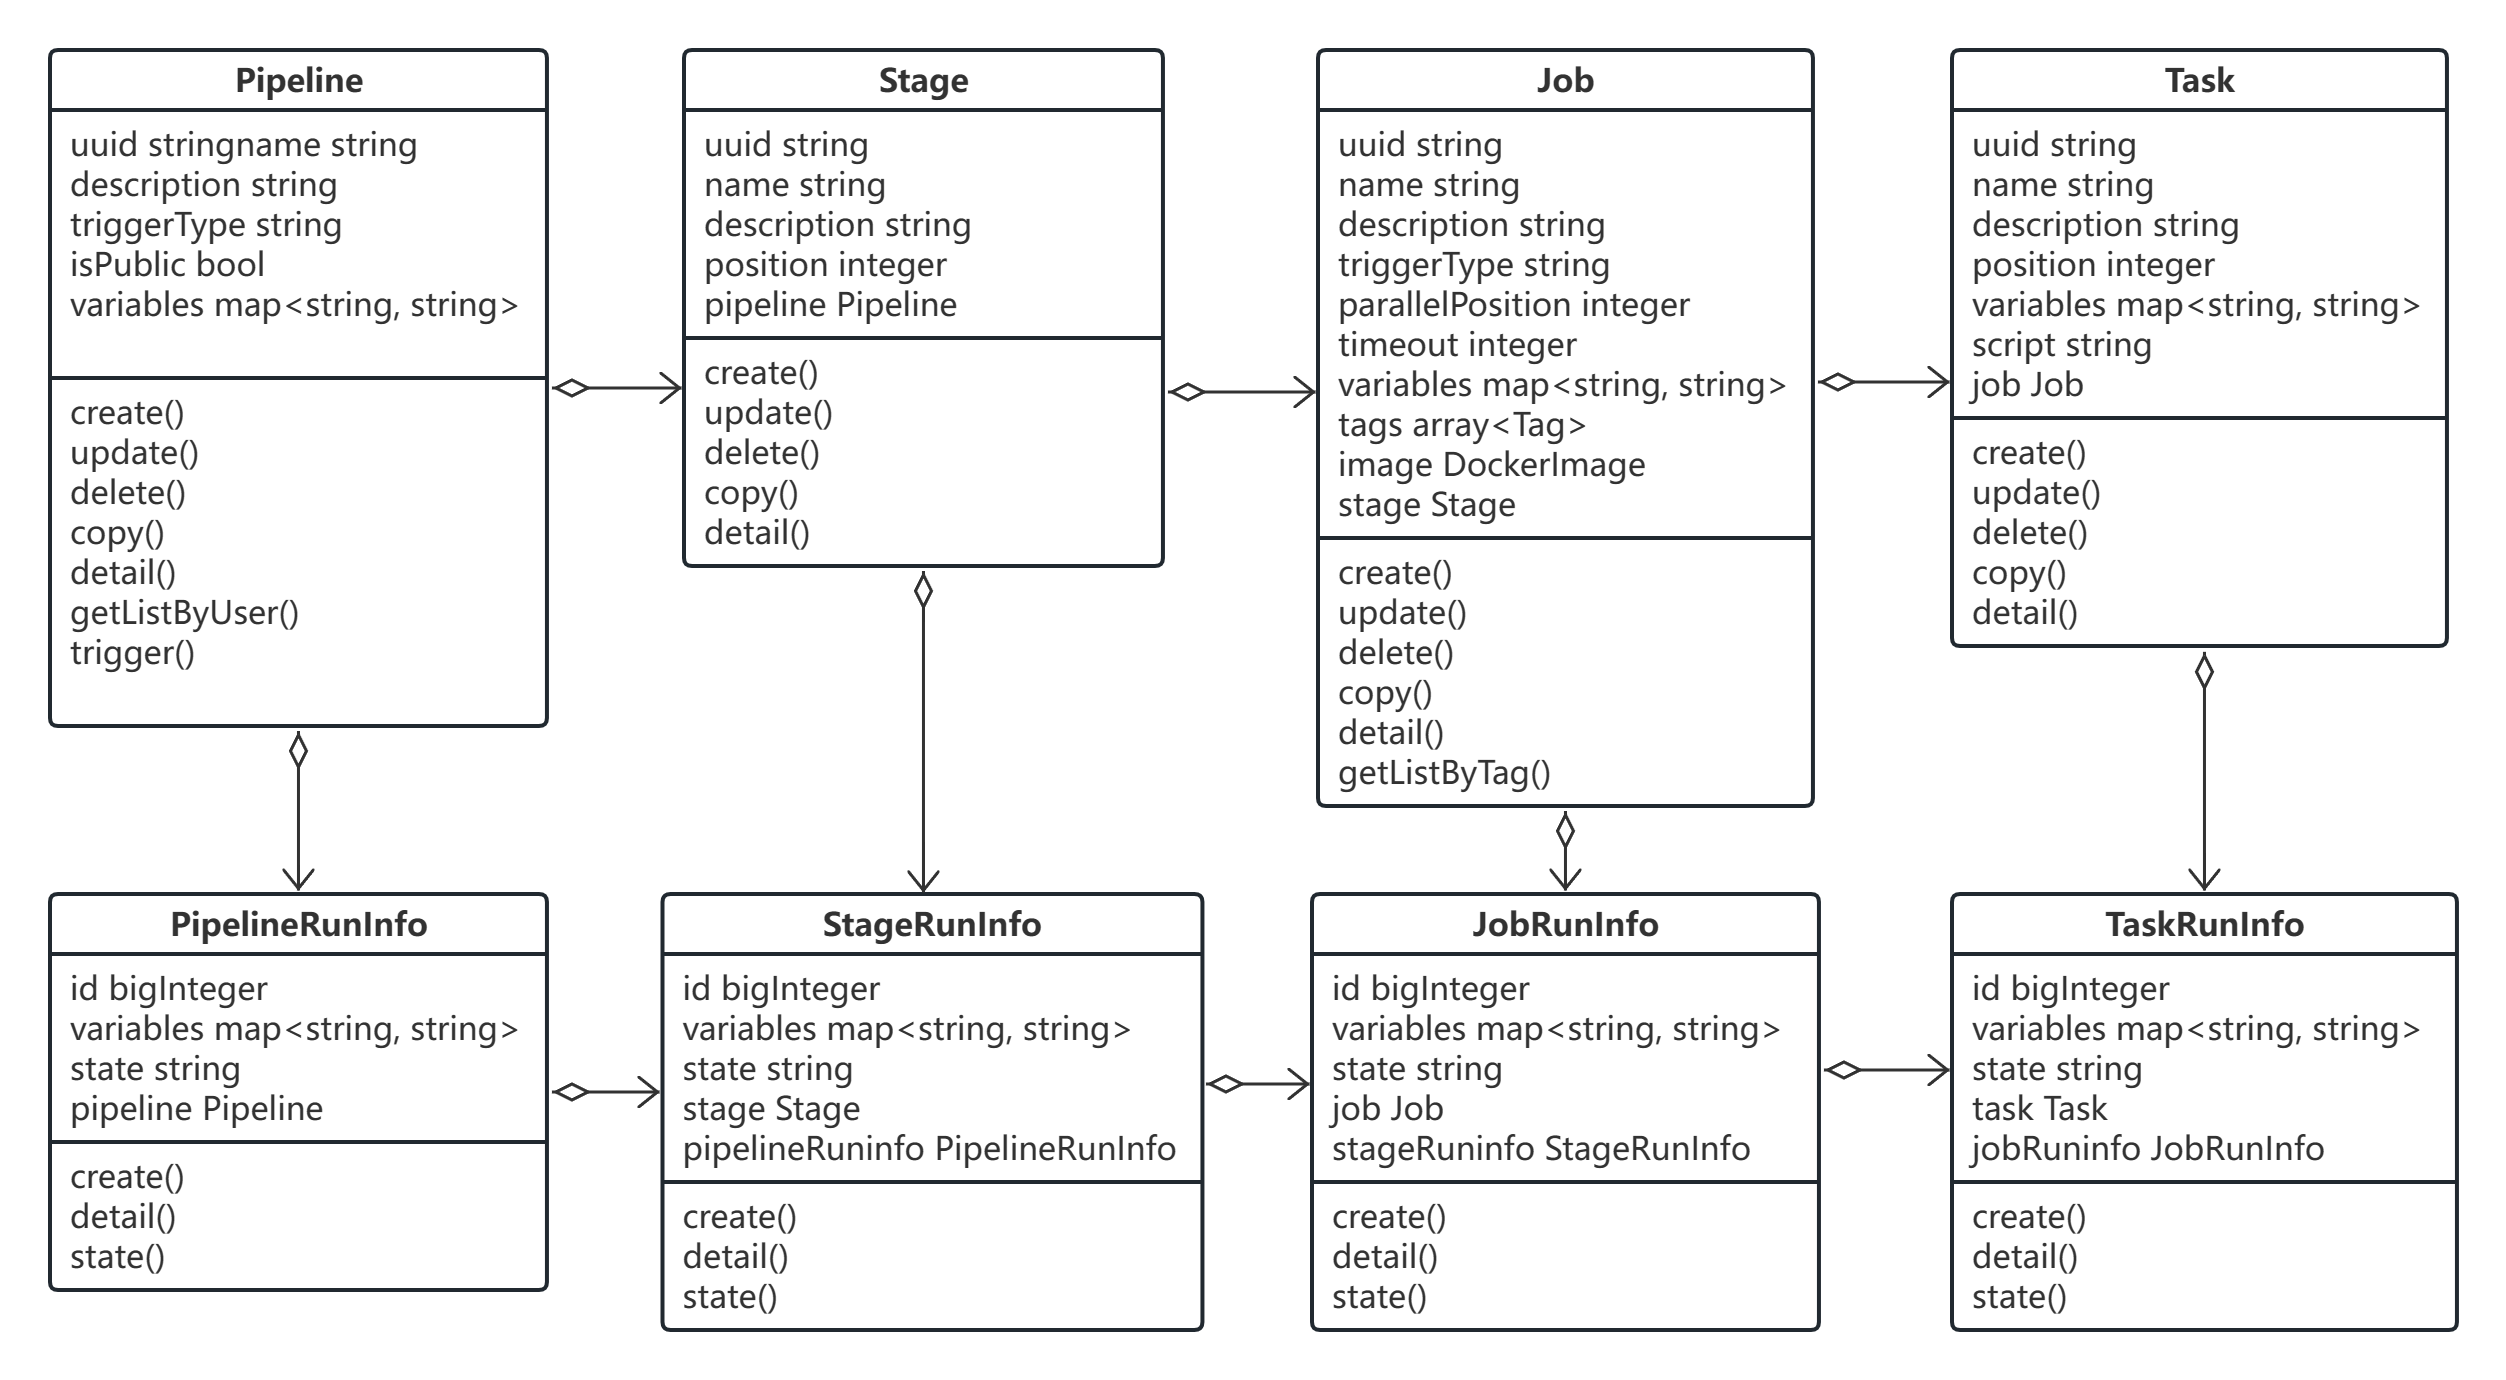
\includegraphics[width=1\textwidth]{流水线管理类图.png}
  \caption{流水线管理类图}
  \label{fig:流水线管理类图}
\end{figure}

\subsection{创建并配置流水线}

用户创建流水线时,系统会调用Pipeline.create()创建出一个空白的初始化流水线,同时其中会递归地调用一次Stage.create()方法创建其内部的一个阶段,
同理Job.create()和Task.create()也会被调用。在流水线管理的相关类中,Pipeline类的大部分成员方法都会递归地向下层调用其所属的子概念实体的对应方法,
以保证增删改查对于整个流水线均生效。当用户创建作业时,在填写基本信息的基础上,还需要在系统所管理的镜像库中指定一个镜像,该作业会在该镜像进行构建出的容器中执行,
如果用户没有合适的镜像选择,系统将会暂存当前用户所构建的流水线配置和结构,跳转到镜像管理界面来引导用户创建镜像。
同时,用户需要为作业指定合适的Tag标签,作业的运行环境可能需要在指定的服务器上运行,以满足其硬件环境要求,作业会通过消息队列被分配到Tag匹配的节点中运行。
每当用户保存当前已经创建并配置好的流水线时,系统都会实时调用Pipeline.detail()方法,以保证用户能够实时查看到当前的流水线配置。

\subsection{触发流水线}

对于流水线的触发,首先将从流水线实体开始调用Pipeline.trigger()方法,该方法中将递归地调用其包含的所有阶段实体的Stage.trigger()方法,
此后每个阶段实体会调用其包含的所有作业实体的Job.trigger()方法,同理调用任务实体的Job.trigger()方法。
每个实体的trigger()方法首先会根据自身的属性创建出对应的运行记录对象实体,并调用Pipeline.create()方法,与上述的trigger()方法类似,
这一方法会递归调用其下的PipelineRunInfo、JobRunInfo和TaskRunInfo的create()方法,创建出与流水线嵌套结构相同的运行记录实体,并存储到数据库。

创建运行记录实体的过程完成后,Backend模块将把当前流水线的结构与配置转化为Json格式发送给调度器。
此后由调度器中的作业中心进行接收并调用JobManager.addJob()进行进一步封装后,
交由调度器中的决策中心发出TriggerEvent触发事件,作业中心将调用JobManager.SubmitJob()将作业交付塞入消息队列中。
最后与作业Tag匹配的节点中的执行器将会从消息队列中得到该作业并开始执行。

\section{镜像管理}
镜像管理的实现主要涉及到对Docker镜像及其操作的封装抽象,以及对Layer层的管理。类图如图\ref{fig:镜像管理类图}所示。

\begin{figure}[h]
  \centering
  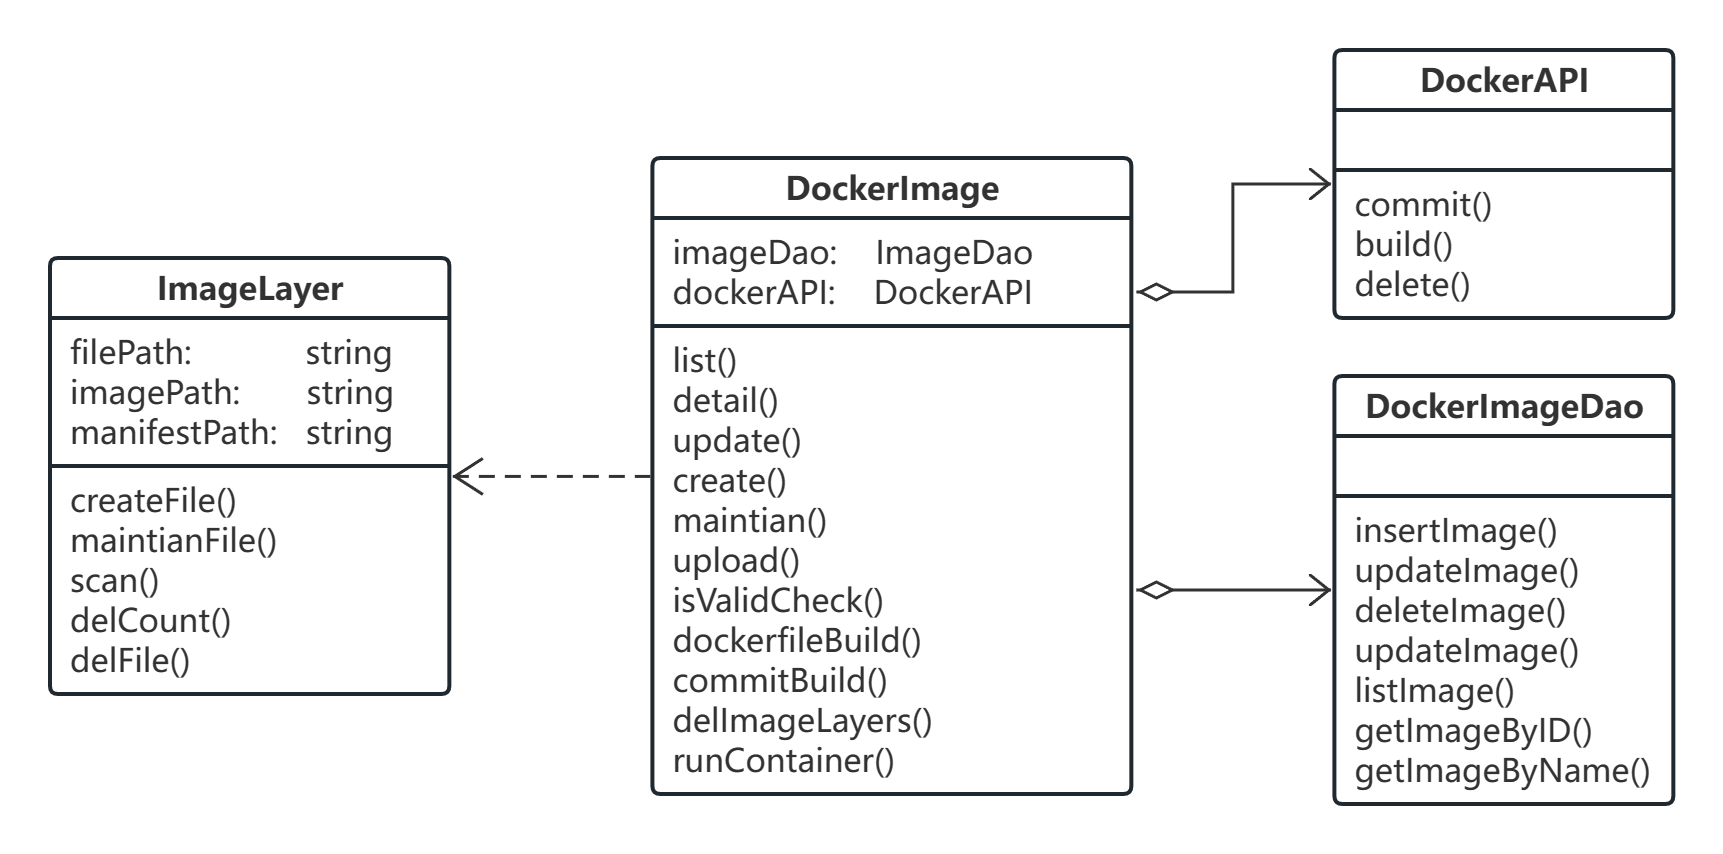
\includegraphics[width=1\textwidth]{镜像管理类图.png}
  \caption{镜像管理类图}
  \label{fig:镜像管理类图}
\end{figure}

\subsection{制作镜像}
制作镜像首先需要用户填写一系列基本信息,包括:镜像名称、镜像描述、镜像标签(Label)等,之后系统会实例化一个DockerImage类对象,
该类对象则包含了一些镜像的属性以及相应操作。

系统首先调用DockerImage.isValidCheck()来检测基础内容是否符合要求,如镜像名称是否有重复,镜像标签是否包含非法字符等。
然后,根据用户传入的制作选项,分别调用不同的制作策略:如果是Dockerfile的策略,系统将调用DockerImage.dockerfileBuild()方法并传入用户传入的文件,
方法内部将ssh进入系统的setting文件中配置的镜像制作服务器,执行docker build命令来直接构建镜像,最后将镜像传入镜像仓库;
如果是Commit策略则首先系统将调用DockerImage.commitBuild()方法,方法内部会在镜像服务器中根据用户配置的基础镜像,执行docker run来启动一个容器,并暴露出容器内部的ssh端口,
此后前端通过Wetty连接容器,此后用户便可以在用户界面使用终端进行操作。
注意,为了保证系统的安全性,我们需要对用户请求进行验证,如果不进行验证,当外部恶意模拟用户请求在服务器中创建容器,并通过一些手段影响到宿主机,会给系统带来极大的安全隐患。

\subsection{上传镜像}
根据在\nameref{subsec:镜像管理}中的分析,为了保证能够充分利用镜像仓库空间,确保不需要的镜像被完全删除,在镜像的上传和删除过程中均需要对Layer进行维护。
首先,前端发送上传镜像请求后,系统将调用DockerImage.upload()方法,该方法内部会判断DockerImage实例对象是否有label属性,根据label标签使用docker push命令推送至不同的仓库,如果没有标签则默认推送至公共仓库。

最后则需要进行Layer操作,首先实例化出ImageLayer实例,调用ImageLayer.scan()方法需要检测Layer文件是否存在,如果不存在则调用ImageLayer.createFile()方法,存在则调用ImageLayer.maintianFile()方法。

ImageLayer.createFile()和ImageLayer.maintianFile()方法会扫描Docker镜像的Manifest文件,将其中引用的ID与Layer实例的ID进行一一比较,从而判断Manifest文件中是否有引用该Layer,如果有则引用数加一,
如果没有则将Layer ID添加到引用文件中并设置引用值为1。这两个方法的区别在于ImageLayer.createFile()需要扫描所有的Manifest文件,而ImageLayer.maintianFile()只扫描指定的Manifest文件。

上传镜像时序图如图\ref{fig:上传镜像时序图}所示。

\begin{figure}[h]
  \centering
  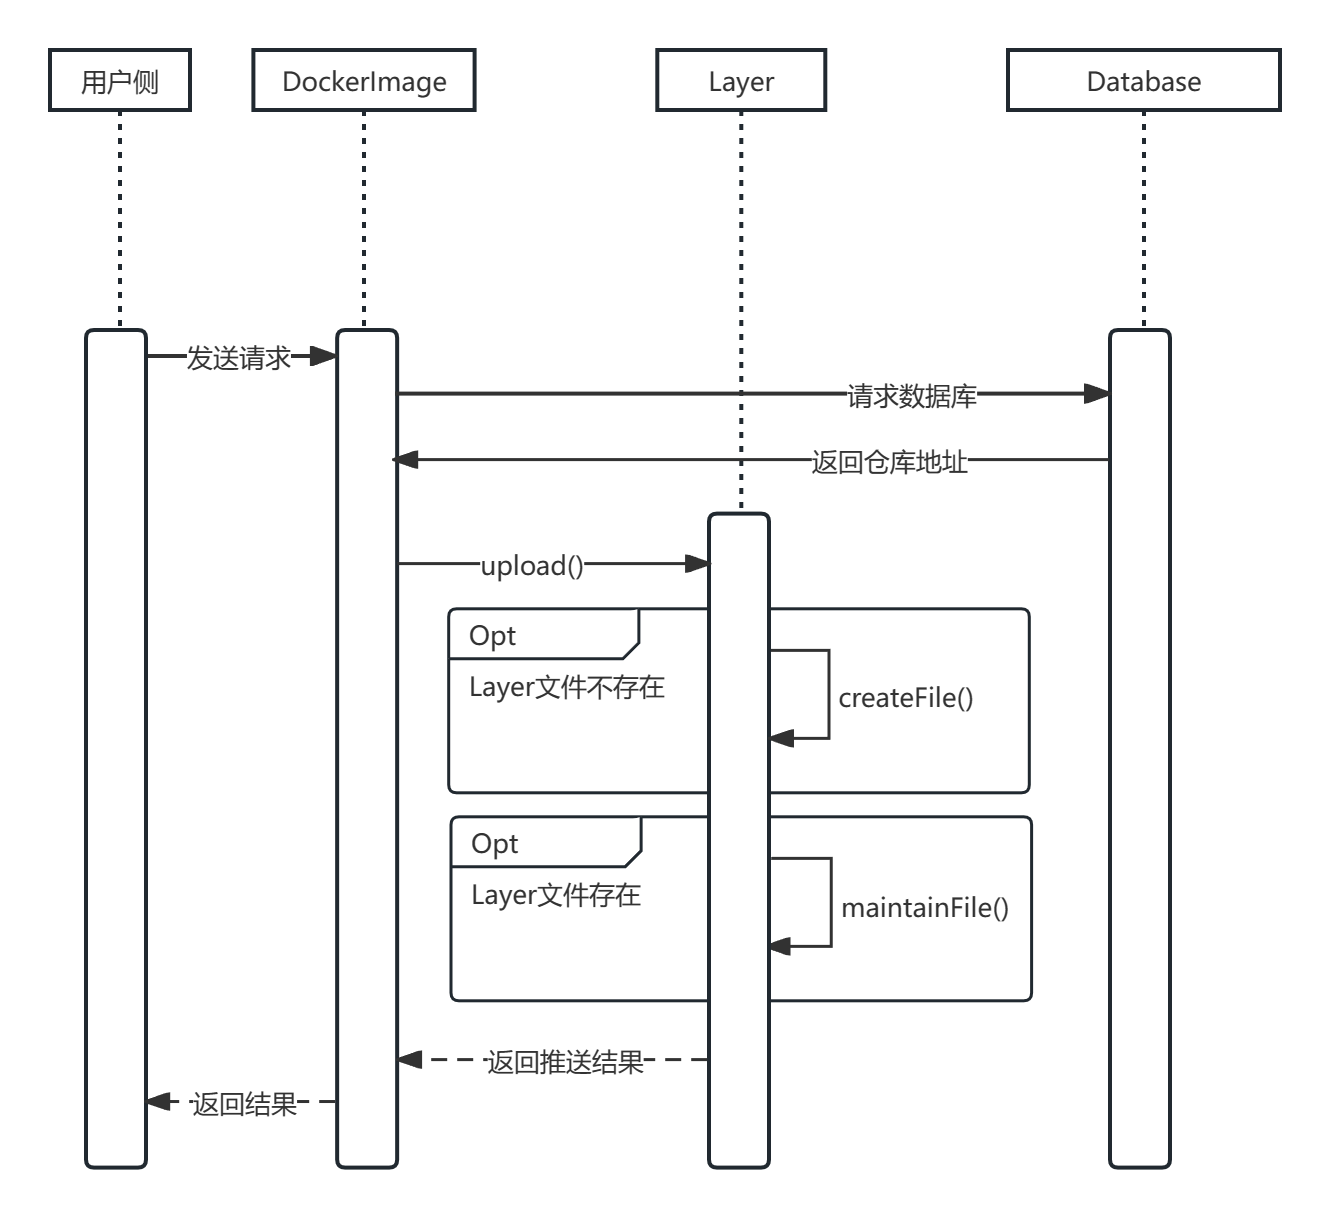
\includegraphics[width=1\textwidth]{上传镜像时序图.png}
  \caption{上传镜像时序图}
  \label{fig:上传镜像时序图}
\end{figure}

\subsection{删除镜像}
镜像由多个镜像层组成,并不是直接存储整个镜像本身,而是存储构成镜像的各个层。
对于每个Docker镜像,私有仓库利用一个Manifest配置文件来记录镜像所依赖的各层信息。当多个镜像共享同一层时,在仓库中该层只会被存储一次。
为解决以上问题,本模块优化了Docker官方的API,克服了无法移除底层文件的限制。这一过程主要包括两个阶段:首先扫描并移除不再需要的镜像层,然后利用Docker API删除相应的Manifest文件。

当需要删除特定镜像时,需对其引用的层进行移除。
我们通过DockerImage.delImageLayers()方法发起移除无效镜像层的请求。
鉴于可能有多个镜像引用同一层的情形,系统必须检查待删除的层是否还被其他镜像所引用。
直接检索每个镜像的Manifest文件以查找层引用会过于复杂,所以系统中为每个镜像层建立一个引用计数文件,记录层的ID和引用次数。
删除镜像时,相应层的引用计数减一。当某层的引用次数降至零时,系统将定位并直接删除该层对应的物理文件。
层的扫描、引用计数的减少及物理文件的删除分别由Layer.layerScan()、Layer.delCount()、Layer.delLayerFile()方法完成。

在移除引用计数文件和层文件之后,最后需调用Docker API来删除对应的Manifest文件,实现Manifest文件的最终删除。


\section{节点管理}
节点管理中对节点、标签和节点部署器中的属性与操作进行了封装抽象,其中节点部署器封装了一系列与节点服务器交互的方法,借助ShellHelper工具类完成使用shell语句与服务器间的交互。
类图如图\ref{fig:节点管理类图}所示。其中ShellHelper类是Shell语句的封装辅助类,将具体的shell语句与业务代码解耦。
Deployer则封装了节点管理中一切与节点服务器交互的方法,将服务器操作与Pod操作类解耦。
Pod类则表示了一个节点对象,与数据库中的一个一条节点记录一一对应,封装了一系列节点属性与节点操作。

接下来重点介绍节点的部署的详细设计。

\begin{figure}[h]
  \centering
  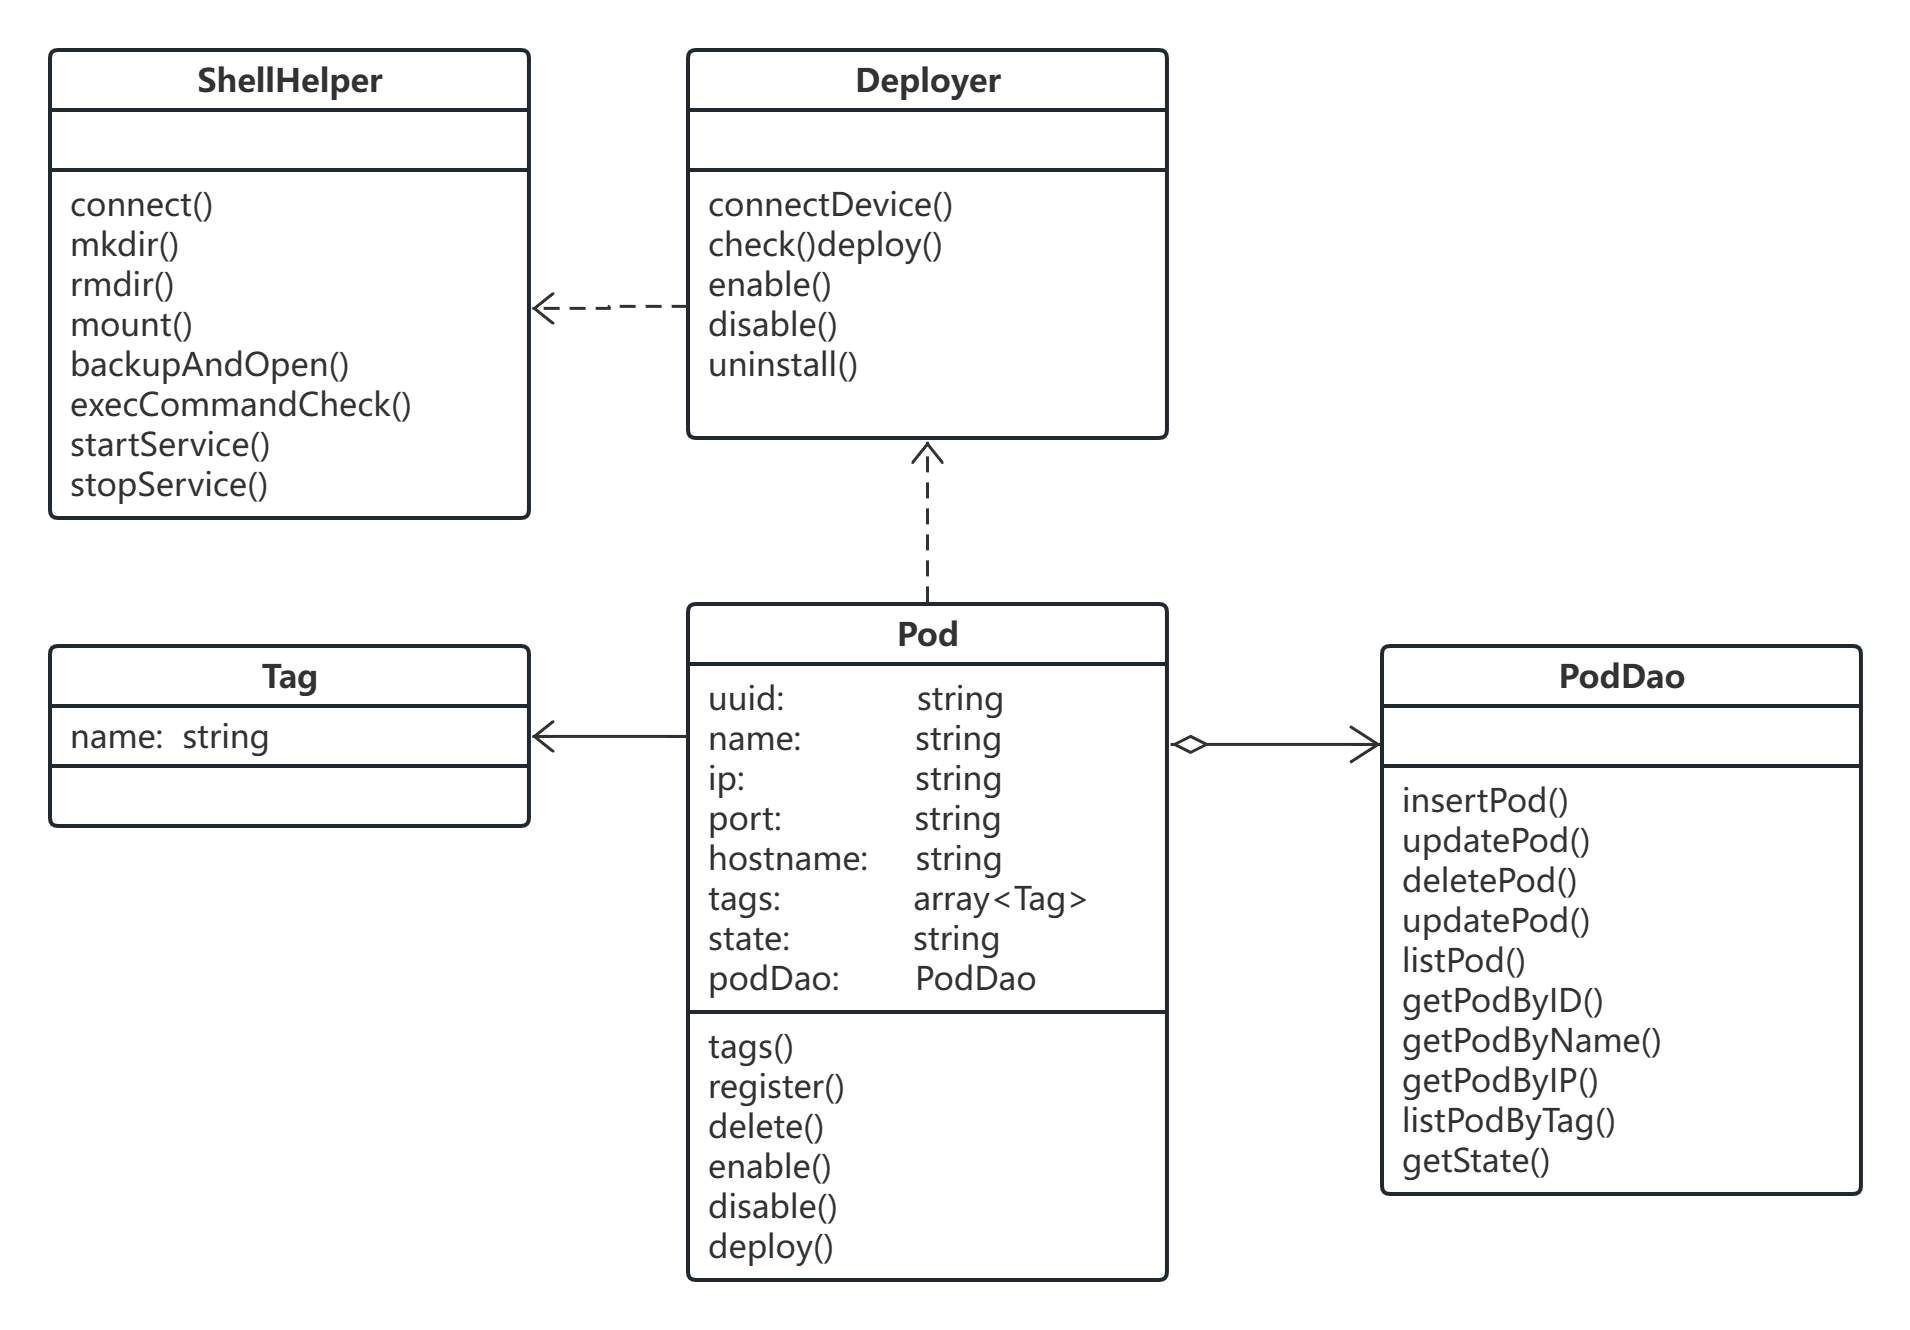
\includegraphics[width=1\textwidth]{节点管理类图.png}
  \caption{节点管理类图}
  \label{fig:节点管理类图}
\end{figure}

\subsection{节点一键部署}
首先,系统在ShellHelper类中设计了execCommandCheck()私有方法,这一方法包含了执行shell语句和检查shell语句两个功能,
如果shell语句执行过程中报错,会根据不同的错误类型返回不同的错误码,这一私有方法在其他方法中被大量调用。
其余ShellHelper类中的方法则是对递归创建文件、启动服务、停止服务等语句的封装,以供Deployer调用。

在节点部署的核心过程如下:首先需要调用ShellHelper.connectDevice()连接到目标服务器,然后递归创建预设的一系列目录结构,并备份原配置文件为bak文件,
分别由ShellHelper中mkdir()和backupAndOpen()方法实现。此后根据执行器的预设yaml文件对服务器配置文件进行写入,同时使用curl命令从远程拉取执行器的二进制执行文件。
此后便可以通过调用ShellHelper.startService()方法,该方法中包含三个部分:首先执行systemctl daemon-reload命令来重新加载配置文件,以保证执行器的配置是最新的,
然后执行systemctl enable来启动执行器服务,最后,自动化部署脚本中,还要执行systemctl restart以便确保所有配置的更改都被采用,并且服务是按照最新配置运行的。

\section{调度器的实现}

\subsection{状态转移模块的实现}

调度器中以状态机的设计模型来控制流水线中作业和任务的状态流转。
以下介绍作业状态机的详细设计,任务状态机与作业状态机极为相似,此处不再赘述。

按照有限状态机的设计理念,我们首先需要确定作业状态机的状态(State)和事件(Event)。
依据需求分析,系统中设计了以下作业状态:就绪中(Pending)、执行中(Running)、执行成功(Success)、执行失败(Failed)、被跳过(Skipped)和被取消(Canceled)。
同时设计了以下事件:触发(triggerEvent)、重试(retryEvent)、作业成功(successEvent)、作业失败(failEvent)、作业执行超时(timeoutEvent)、跳过(skipEvent)、取消(cancelEvent)、审核通过(reviewApproveEvent)和审核失败(reviewRejectEvent)。
依据状态机的设计模式,系统中将流水线作业的不同状态封装为类,将引起其状态转移的事件设置为成员方法。图~\ref{fig:作业状态机类图}为作业状态机类图。

\begin{figure}[h]
  \centering
  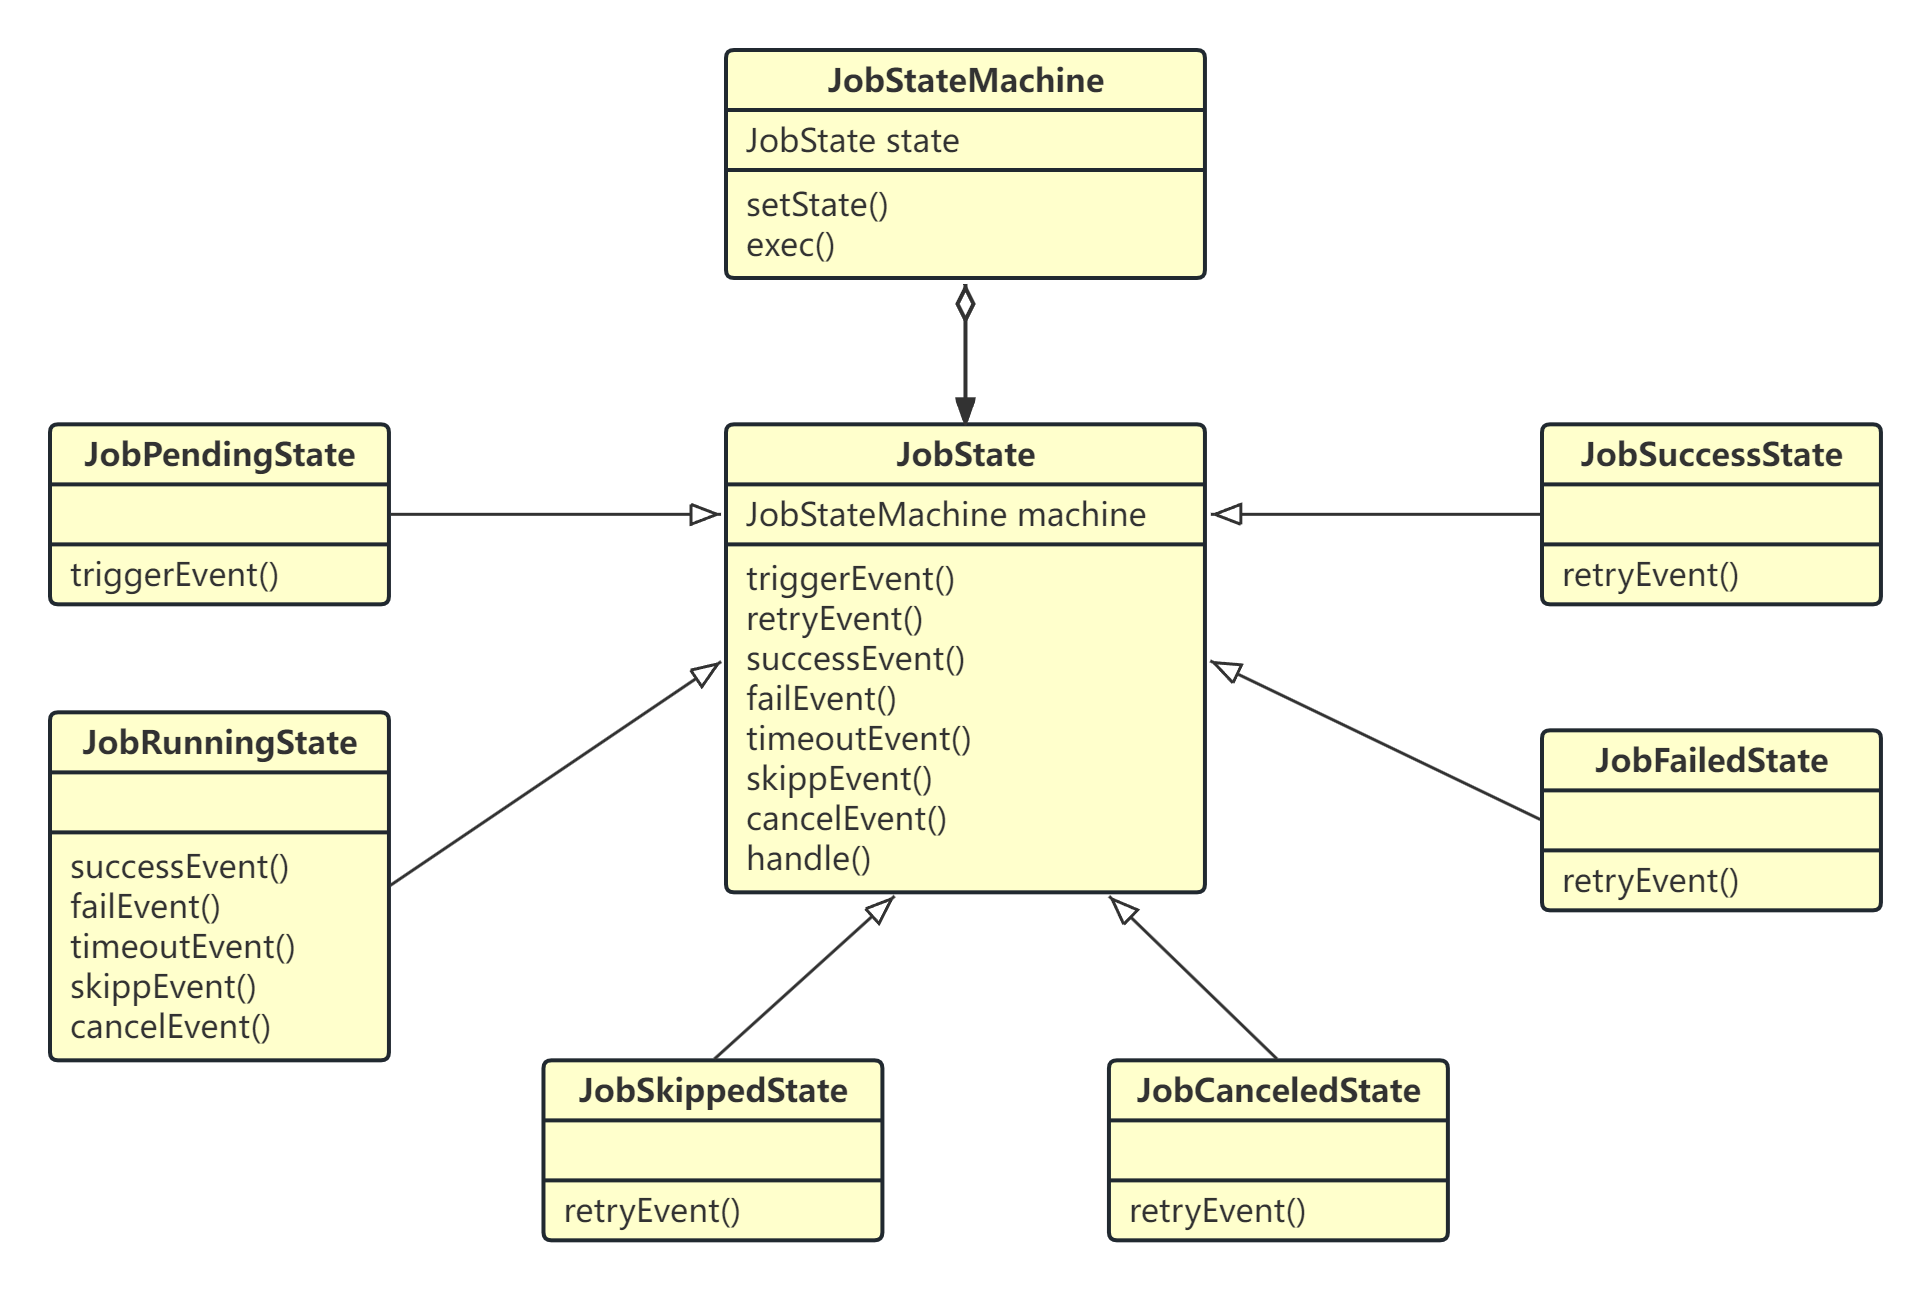
\includegraphics[width=1\textwidth]{作业状态机类图.png}
  \caption{作业状态机类图}
  \label{fig:作业状态机类图}
\end{figure}

当需要进行作业状态转换时,首先创建JobStateMachine实例并设置默认初始状态,然后向exec成员方法中传入当前发生的事件。
其中JobState是作业状态的抽象类,作业中每个具体的状态作为一个JobState的实现类,并从JobState中选择引起其状态转移的事件方法来实现。
例如JobRunningState类实现了JobState中的successEvent、failEvent、timeoutEvent、skippEvent和cancelEvent五个成员方法,这是因为这些事件均能作用于一个正在运行中的作业并且引起其状态改变,
其中successEvent方法会调用父类中持有的实例的JobStateMachine成员的setState方法,将当前状态机的状态设置为成功,并完成一些后续工作,其余事件方法也与之类似。

接下来具体分析作业状态机内部的状态转换:
当一个作业运行实例被创建时其应为就绪中状态,故就绪中(Pending)状态为初始状态,引发其状态改变的事件是触发(triggerEvent),这个触发事件是由决策中心经过决策逻辑发出的,并不只是用户的动触发行为,
一旦作业被成功触发,其状态则改变为运行中(Running);如果该作业被设定为需要人工审核才能触发,则审核通过事件(reviewApproveEvent)将会将状态改变为运行中(Running),审核驳回事件(reviewRejectEvent)将会将状态改变为失败(Failed)。
当作业处于运行中时,调度器可能会收到来自两方面的信号,其一是执行器所通知的作业执行状态,包括作业执行成功(successEvent)、执行失败(failEvent)和执行超时(timeoutEvent),
其中执行成功会使得作业状态机变为执行成功状态(Success),执行失败和执行超时都会变为执行失败状态(Failed);
其二是CI-Service所通知的用户人工干预命令,包括取消作业(cancelEvent)和跳过(skipEvent)作业,这两种事件会立即使得作业状态机变为取消(Canceled)和跳过(Skipped)状态。
以上两种信号均由决策中心先收到信号并统一处理决策后再转发给状态机,这样做可以统一外界信号的入口,降低其他模块与调度器间的耦合。
当处于运行中的作业进入终态后,作业仍然可以通过重试事件(retryEvent)来重新进入运行中的状态。
至于当前的作业是否满足触发该事件的条件,或者是否需要人工审核,由决策中心统一处理后发出信号,状态机不做额外的业务逻辑判断。

图~\ref{fig:流水线作业状态图}展示了作业状态机的状态流转。

\begin{figure}[h]
  \centering
  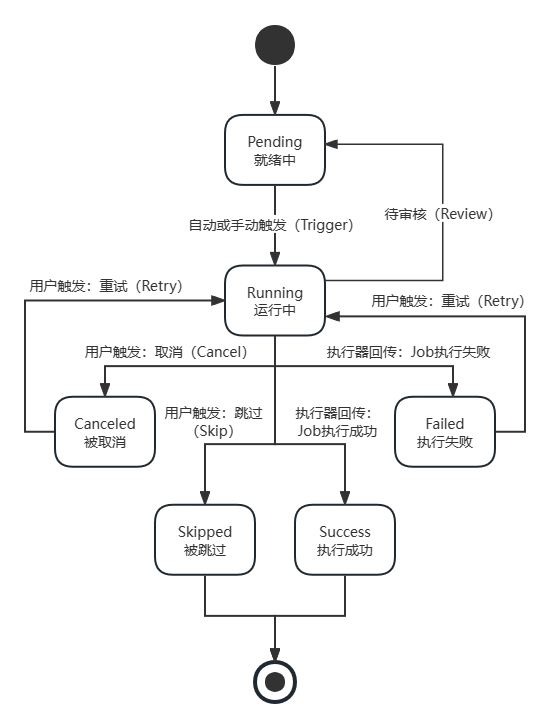
\includegraphics[width=0.7\textwidth]{流水线作业状态图.png}
  \caption{流水线作业状态图}
  \label{fig:流水线作业状态图}
\end{figure}

% 对于流水线和阶段的状态转移则相对比较简单。
% 对于阶段来讲,阶段的状态并不受到的具体的作业运行情况的影响,而是根据当前该阶段内所有作业的状态来综合决定,阶段状态机的类图如图\ref{}所示。

% 首先我们需要定义一套

\subsection{作业管理与决策中心模块的实现}

作业管理是调度器对Backend模块传入的作业信息进行二次封装和操作的模块。
决策中心则是整个调度器的核心模块,负责根据当前发生的事件(Event)和当前作业状态对作业管理模块中获得的作业进行决策。
作业管理与决策中心的类图如图\ref{fig:作业管理与决策中心类图}所示。

\begin{figure}[h]
  \centering
  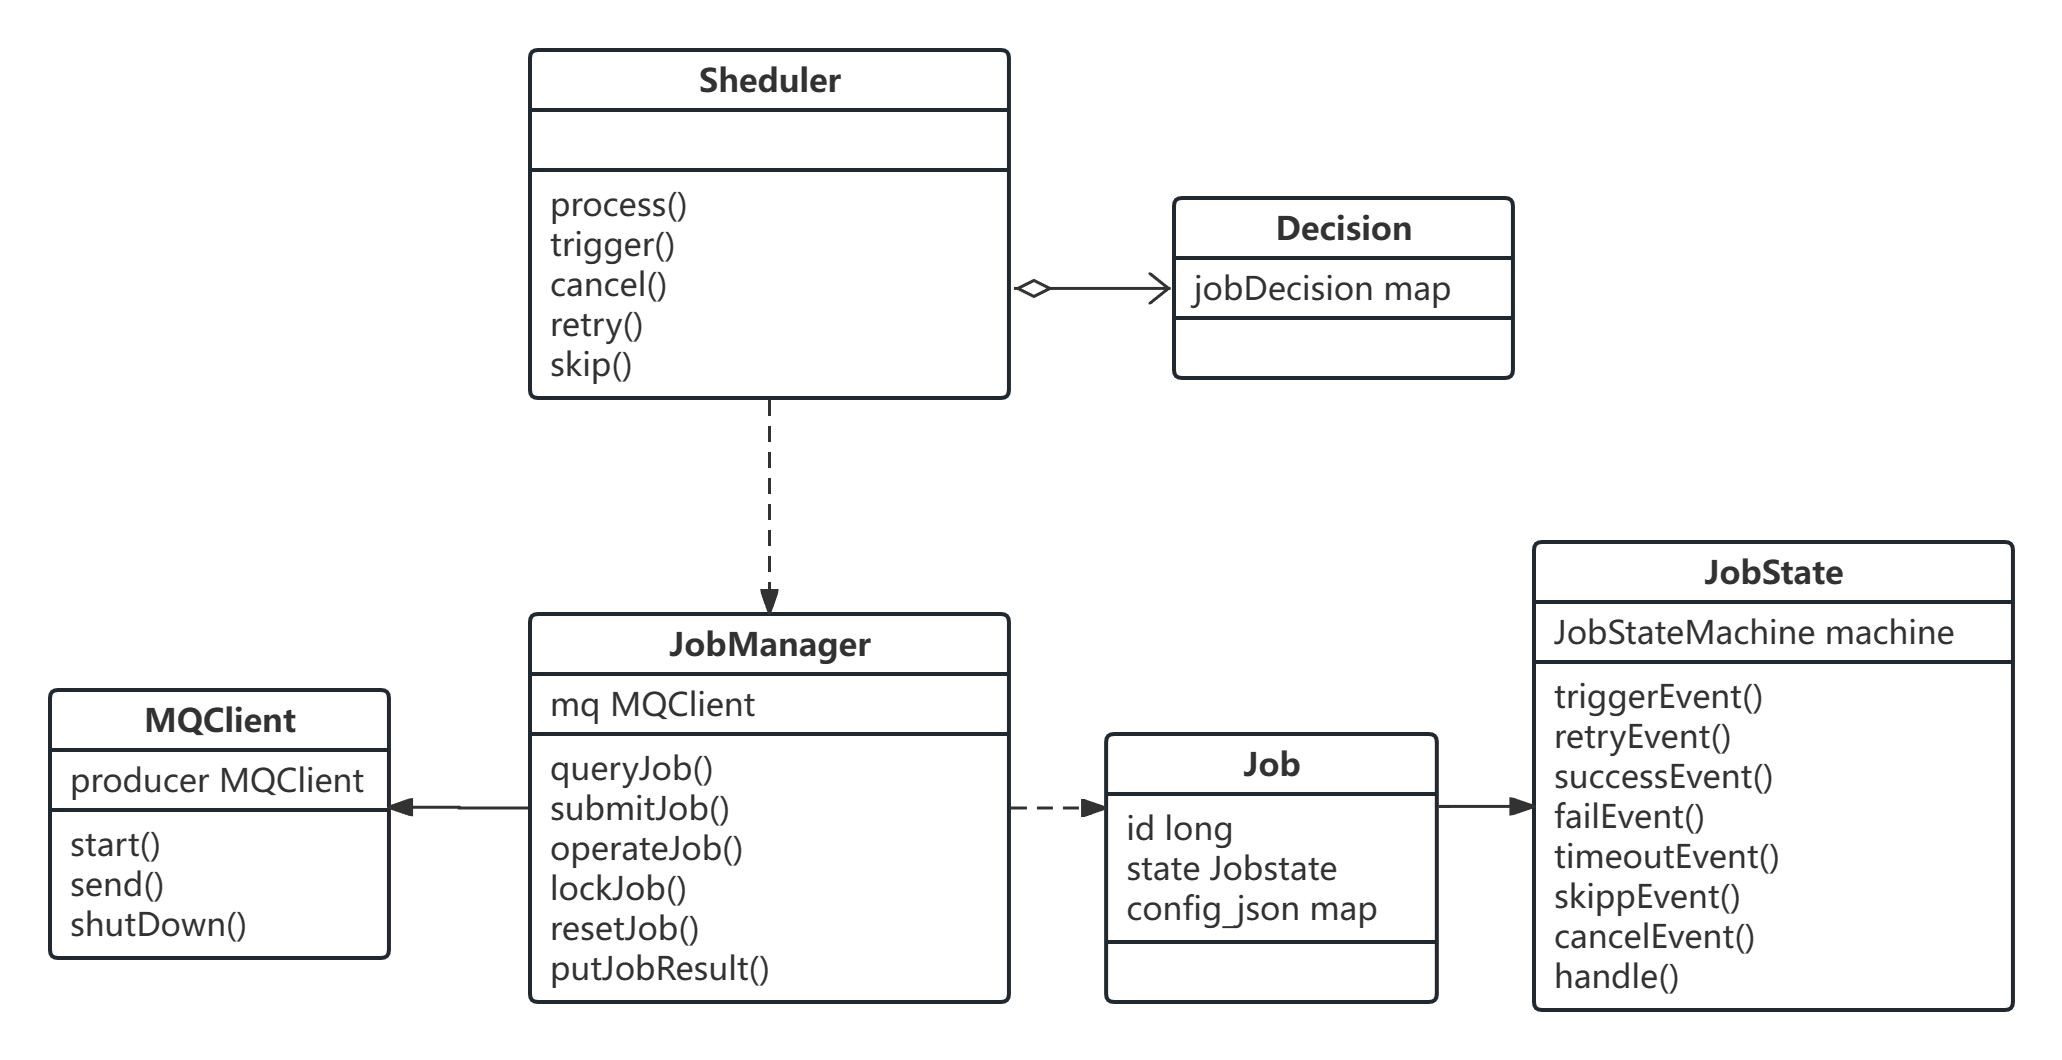
\includegraphics[width=1\textwidth]{作业管理与决策中心类图.png}
  \caption{作业管理与决策中心类图图}
  \label{fig:作业管理与决策中心类图}
\end{figure}

在整个调度器的核心代码中,Scheduler 类位于调度模块的核心位置,其主要负责执行一个关键功能:processTask()。该方法的主要职责是从作业管理器中拉取待处理的作业,并基于作业事件及其当前状态来做出相应的调度决策。
makeRunDecision()方法体现了该决策逻辑,而当决策包含特定的作业处理时,batchPutJobDecision则被用于执行相关操作。决策对象由Decision类封装,其中作业的决策以Map形式存在,以便支持作业的并行处理能力。
这其中会用到一个DecisionEnum枚举类,其中包含可能的决策事件并与作业状态机中的Event一一对应,这些事件直接影响流水线作业的执行和作业状态的转换。

作业管理(JobManager)和Scheduler交互是通过作业实体Job进行的,putJobResult()方法接受执行器返回的状态更新,并将相关作业重新排队等待下一轮调度决策。getUnackJobs()方法能够查询那些已经分发给执行器但尚未执行的作业。

系统初始化时,Scheduler.process()方法将在守护线程中运行,不断地处理作业。当Backend服务接收到用户发起的流水线事件时,会通过addJob()方法将作业提交至消息队列中进行排队。
此处需要注意,由于系统中调度器是多实例部署,属于分布式系统,任何一个节点都有可能处理这些作业,如此便产生了竞态条件,为了避免发生无法预期的错误,
以及保证作业不丢失,在进行决策前,必须通过JobManager.lockJob()方法对作业加锁,以获得处理权。

Scheduler在接收到一批待处理作业后,会根据每个作业的具体事件类型及其包含的状态进行详细决策。
完成决策后,决策结果Decision将被检查,如果包含对作业的决策,则将其发送回作业管理器以便进一步处理,这可能会导致作业状态的变更,则交由JobStateMachine进行处理。
若决策中未包含对整个作业的处理,而是针对特定作业的,则会触发作业管理器的相关处理逻辑,并通过后端服务进行状态持久化。
最后调用JobManager.releaseJob()对锁进行释放。

结合以上内容,作业调度时序图如图\ref{fig:作业调度时序图}所示。

\begin{figure}[h]
  \centering
  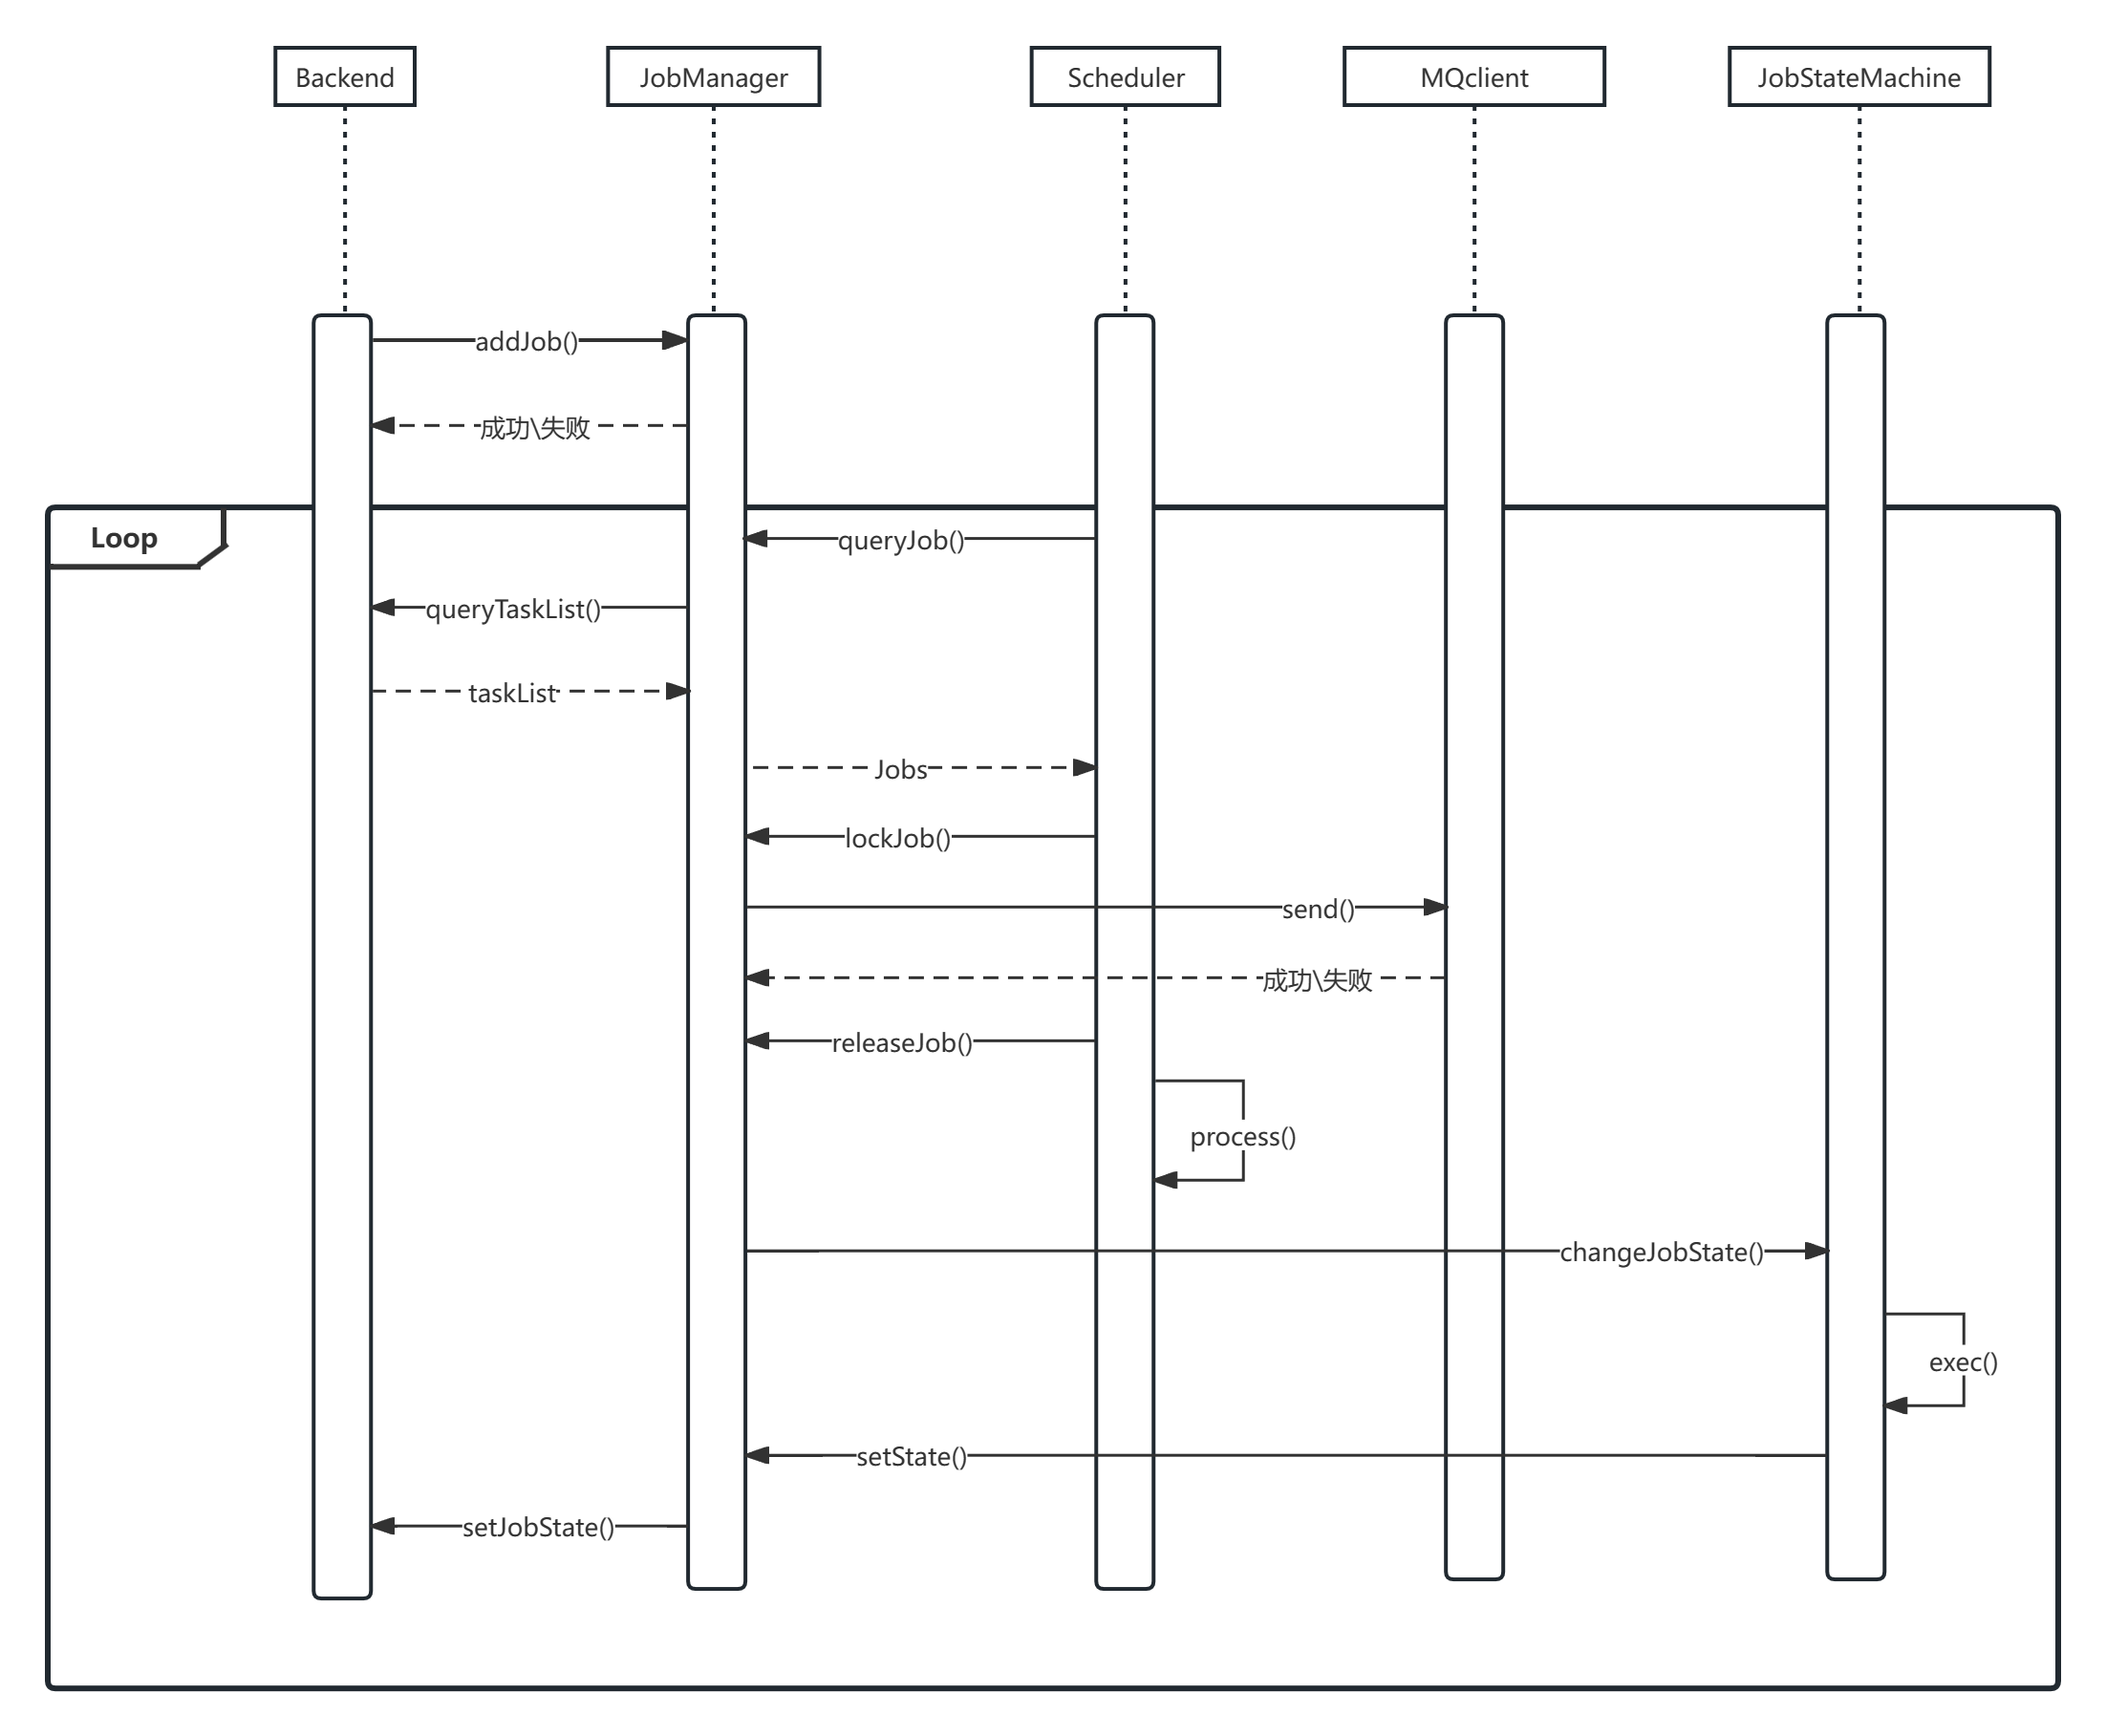
\includegraphics[width=0.8\textwidth]{作业调度时序图.png}
  \caption{作业调度时序图}
  \label{fig:作业调度时序图}
\end{figure}

\section{本章小结}
在本章中,我们深入探讨了容器化CI/CD流水线调度系统的详细设计与实现,重点关注了系统内部的算法、数据结构及其相互作用。
首先,流水线管理部分通过详细的类图和实例方法展示了如何高效地处理流水线的创建、配置与触发。特别是通过递归调用的设计,实现了从流水线到阶段、作业、任务的层层下达与信息同步,保证了流水线配置的一致性和执行的准确性。
镜像管理部分详述了如何在系统中创建、上传和删除Docker镜像。通过引入Layer层的概念,系统不仅简化了镜像管理过程,还优化了存储使用,提高了系统的整体效率和镜像的处理速度。
节点管理部分着重介绍了节点的一键部署功能,包括与节点服务器的交互、执行器的安装和配置,以及节点的上线与下线处理。此外,还强调了通过ShellHelper辅助类实现与服务器交互的灵活性和安全性。
调度器的实现部分则集中于系统的核心逻辑,即如何根据作业的状态和事件来做出合理的调度决策。通过有限状态机的设计模型,系统能够精确控制作业和任务的状态转换,同时确保作业的有序执行和资源的合理分配。
整体而言,本章从算法到数据结构,从功能设计到实现细节,为系统的构建提供了全面而深入的技术支撑,确保了系统的高效、稳定和可扩展。
% !TeX root = ../main.tex

\chapter{系统测试}
一些废话
\section{测试环境}
系统中需要部署的服务包括

\section{功能测试}
本小节对系统的三个功能模块中的各个具体用例进行测试,并以测试用例的形式对过程进行了说明。

首先对流水线管理模块进行测试,这一模块的测试点主要在于对流水线的增删改查、配置项配置和人工干预操作,
尤其是触发人工干预操作后,检查状态转移是否符合预期,作业执行过程中的日志和产物是否得到了保存等。

设计作业管理测试用例时,检查点主要有对流水线及其各个子概念的创建、编辑、删除和查看,结果均符合预期,如表\ref{tab:作业管理测试用例表}所示。

\begin{table}[ht]
  \centering
  \caption{作业管理测试用例表}
  \label{tab:作业管理测试用例表}
  \begin{tabular}{|p{1.5cm}|p{2.5cm}|p{3cm}|p{3cm}|p{1.5cm}|}
  \hline
  \multicolumn{1}{|p{1.5cm}|}{测试模块} & \multicolumn{4}{l|}{流水线管理} \\ \hline
  \multicolumn{1}{|p{1.5cm}|}{模块功能} & \multicolumn{4}{l|}{流水线的配置、编辑和查看} \\ \hline
  \multicolumn{1}{|p{1.5cm}|}{测试目的} & \multicolumn{4}{l|}{验证系统是否能正确地对流水线进行配置} \\ \hline
  用例编号 & 检查点 & 操作步骤 & 预期输出 & 结果 \\ \hline
  1-1-1 & 创建流水线 & 1、进入“我的流水线”Tab页,点击“创建”按钮; \newline 2、录入流水线基本设置; \newline 3、点击“保存”按钮。 & 1、出现创建成功提示信息; \newline 2、在UI界面中看到流水线记录。 & 符合预期 \\ \hline
  1-1-2 & 创建流水线\newline——创建阶段 & 1、在用例1-1-1中切换至拓扑编辑Tab页; \newline 2、在已有的初始阶段上录入基本设置; \newline 3、点击加号增加几个新的阶段并录入基本设置。 & 在流水线的拓扑结构UI界面中看到新创建的阶段 & 符合预期 \\ \hline
  1-1-3 & 创建流水线\newline——创建作业 & 1、在用例1-1-2中点击创建的阶段中的加号; \newline 2、录入基本设置。 & 在流水线的拓扑结构UI界面中看到新创建的作业 & 符合预期 \\ \hline
  1-1-4 & 创建流水线\newline——创建任务 & 1、在用例1-1-3中点击创建的作业中的加号; \newline 2、录入基本设置。 & 在流水线的拓扑结构UI界面中看到新创建的任务 & 符合预期 \\ \hline
  1-2-1 & 编辑流水线 & 1、在“我的流水线”Tab页,在对应流水线处点击“编辑”按钮; \newline 2、修改基本设置; \newline 3、修改拓扑结构。 & 配置页和拓扑结构页的内容更新为编辑后的新内容 & 符合预期 \\ \hline
  1-3-1 & 删除流水线 & 1、在“我的流水线”Tab页,在对应流水线处点击“删除”按钮; \newline 2、在提示弹窗中点击“确认”按钮。 & 出现删除成功提示信息 & 符合预期 \\ \hline
  1-4-1 & 查看流水线配置 & 进入“我的流水线”Tab页,点击“查看”按钮。& 在UI界面中显示了流水线拓扑结构和基本配置 & 符合预期 \\ \hline
  \end{tabular}
\end{table}

在对流水线进行适当的增删改查后,系统中成功创建了一条流水线,流水线管理模块功能符合预期,如图\ref{fig:流水线截图}所示,该流水线是对示意图\ref{fig:典型流水线示意图}的实现。
接下来将根据该流水线进行人工干预测试,验证其状态转移是否符合预期。

\begin{figure}[h]
  \centering
  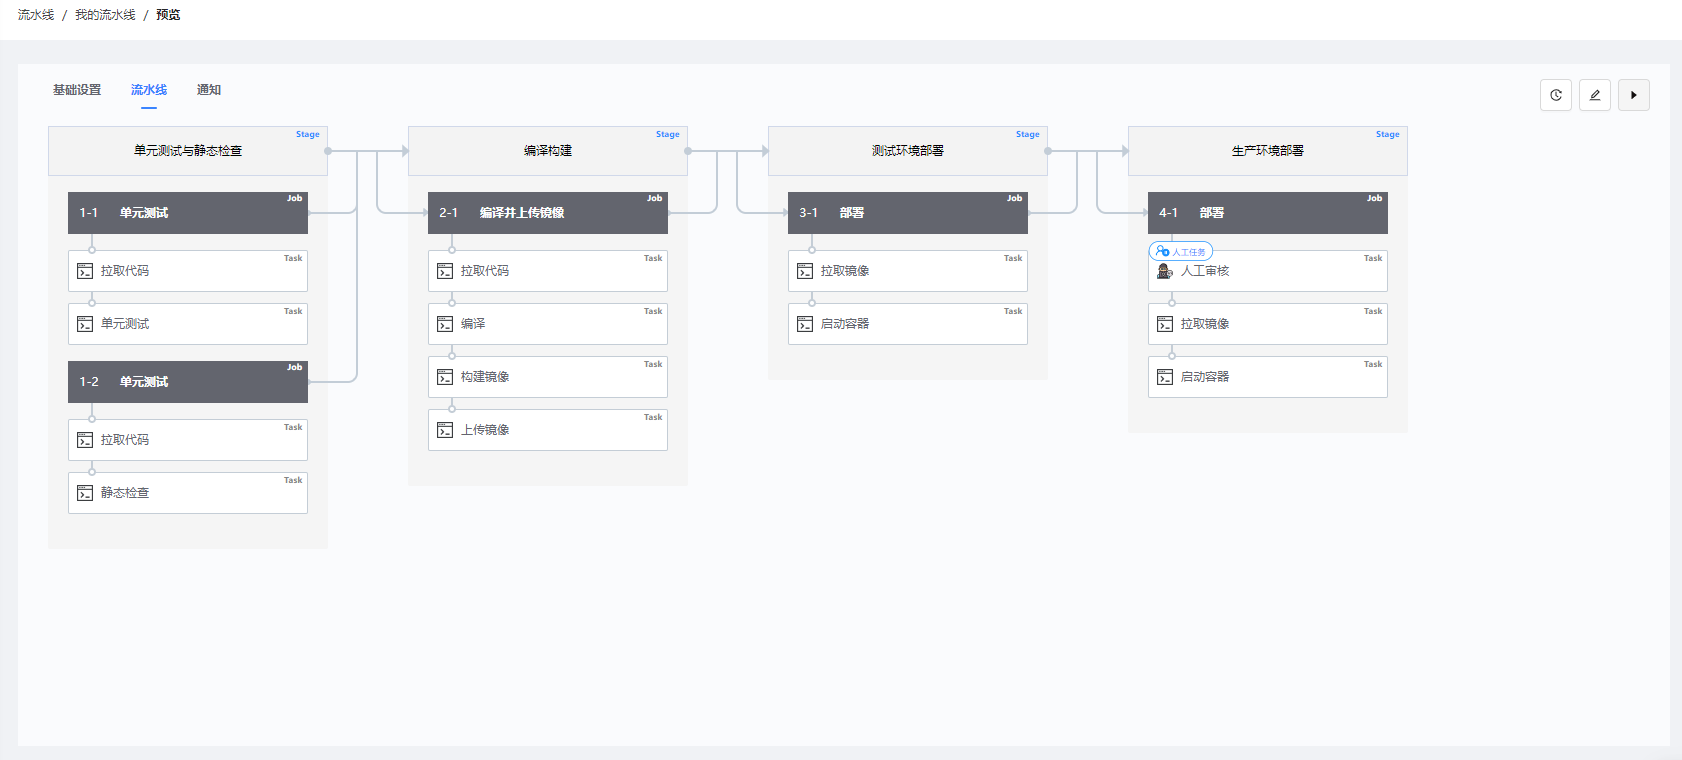
\includegraphics[width=1\textwidth]{流水线截图.png}
  \caption{流水线截图}
  \label{fig:流水线截图}
\end{figure}

对于人工干预流水线,主要的检查点是对流水线及其各个子概念的触发、跳过、重试、取消和人工审核,经过测试,结果均符合预期,如表\ref{tab:人工干预测试用例表}所示。

\begin{table}[ht]
  \centering
  \caption{人工干预测试用例表}
  \label{tab:人工干预测试用例表}
  \begin{tabular}{|p{1.5cm}|p{2.5cm}|p{3cm}|p{3cm}|p{1.5cm}|}
  \hline
  \multicolumn{1}{|p{1.5cm}|}{测试模块} & \multicolumn{4}{l|}{人工干预} \\ \hline
  \multicolumn{1}{|p{1.5cm}|}{模块功能} & \multicolumn{4}{l|}{流水线、阶段、作业的触发、跳过、重试、取消和人工审核} \\ \hline
  \multicolumn{1}{|p{1.5cm}|}{测试目的} & \multicolumn{4}{l|}{验证人工干预后系统的状态流转与作业执行是否符合预期} \\ \hline
  用例编号 & 检查点 & 操作步骤 & 预期输出 & 结果 \\ \hline
  2-1-1 & 触发流水线 & 1、进入图\ref{fig:流水线截图}所示的流水线预览页面; \newline 2、点击“触发”按钮。& 1、出现触发成功提示信息; \newline 2、在UI界面中看到流水线中作业的运行日志和状态流转。 & 符合预期 \\ \hline
  2-2-1 & 取消流水线 & 在用例2-1-1流水线执行页面中点击“中止”按钮。 & 流水线状态变为已取消,当前正在执行的作业状态变为已取消 & 符合预期 \\ \hline
  2-3-1 & 取消阶段 & 在用例2-1-1中点击正在执行中的阶段上的“中止”按钮。 & 指定的阶段状态变为已取消,阶段内的所有未执行完的作业状态变为已取消 & 符合预期 \\ \hline
  2-4-1 & 重试阶段 & 在用例2-3-1中点击被取消的阶段上的“重试”按钮。 & 原本已被取消的阶段变为执行中,阶段内的作业重新开始运行 & 符合预期 \\ \hline

  2-5-1 & 手动触发作业 & 选择类型为手动触发的作业,点击“触发”按钮 & 在节点资源充足的情况下,手动触发作业由就绪中转为执行中 & 符合预期 \\ \hline
  2-6-1 & 人工审核\newline——审核通过 & 选择类型为人工审核的作业的首个任务,点击“通过”按钮 & 在节点资源充足的情况下,人工审核作业由就绪中转为执行中 & 符合预期 \\ \hline
  2-6-2 & 人工审核\newline——审核驳回 & 选择类型为人工审核的作业的首个任务,点击“驳回”按钮 & 人工审核作业由就绪中转为执行失败 & 符合预期 \\ \hline
  2-7-1 & 取消作业 & 在用例2-1-1执行中的流水线上选择正在执行的流水线点击“取消”按钮 & 作业由执行中转为已取消 & 符合预期 \\ \hline
  2-8-1 & 跳过作业 & 在用例2-1-1执行中的流水线上选择正在执行的流水线点击“跳过”按钮 & 作业由执行中转为已跳过,下一个作业开始执行 & 符合预期 \\ \hline
  2-9-1 & 重试作业 & 在用例2-7-1选择已取消的作业上点击“重试”按钮 & 在节点资源充足的情况下,作业由已取消转为执行中 & 符合预期 \\ \hline
  \end{tabular}
\end{table}


\begin{table}[ht]
  \centering
  \caption{镜像管理测试用例表}
  \label{tab:镜像管理测试用例表}
  \begin{tabular}{|p{1.5cm}|p{2.5cm}|p{3cm}|p{3cm}|p{1.5cm}|}
  \hline
  \multicolumn{1}{|p{1.5cm}|}{测试模块} & \multicolumn{4}{l|}{镜像管理} \\ \hline
  \multicolumn{1}{|p{1.5cm}|}{模块功能} & \multicolumn{4}{l|}{镜像的制作、删除与上传} \\ \hline
  \multicolumn{1}{|p{1.5cm}|}{测试目的} & \multicolumn{4}{l|}{验证系统对镜像的操作能否正常执行,镜像服务器中镜像是否正常存储与清理} \\ \hline
  用例编号 & 检查点 & 操作步骤 & 预期输出 & 结果 \\ \hline
  3-1-1 & 制作镜像\newline——dockfile方法 & 1、进入“镜像管理”Tab页,点击“镜像制作”;\newline 2、填写镜像基本信息;\newline 3、上传Dockerfile文件后点击“构建”。& 1、出现制作成功提示信息; \newline 2、在“镜像列表”中查看到新制作的镜像。 & 符合预期 \\ \hline
  3-1-2 & 制作镜像\newline——commit方法 & 1、进入“镜像管理”Tab页,点击“镜像制作”;\newline 2、填写镜像基本信息;\newline 3、选择基础镜像点击“构建”;\newline 4、在终端进行配置操作;5、点击“构建”按钮。 & 1、出现制作成功提示信息; \newline 2、在“镜像列表”中查看到新制作的镜像。 & 符合预期 \\ \hline
  3-2-1 & 编辑镜像 & 1、在用例3-1-1或3-1-2的基础上,点击制作好的镜像上的“编辑”;\newline 2、编辑镜像基本信息后点击“保存”;& 镜像信息更新为编辑后的新内容。 & 符合预期 \\ \hline
  3-3-1 & 上传镜像 & 在用例3-1-1或3-1-2的基础上,点击制作好的镜像上的“上传”。& 1、出现上传成功提示信息;2、在镜像服务器中可以查看到对应镜像。 & 符合预期 \\ \hline
  3-4-1 & 删除镜像 & 在用例3-3-1基础上,点击已上传的镜像点击“删除” & 1、出现删除成功提示信息;2、在镜像服务器上查看对应的Manifest文件和Layer文件已被删除。 & 符合预期 \\ \hline
  \end{tabular}
\end{table}


\begin{table}[ht]
  \centering
  \caption{节点管理测试用例表}
  \label{tab:节点管理测试用例表}
  \begin{tabular}{|p{1.5cm}|p{2.5cm}|p{3cm}|p{3cm}|p{1.5cm}|}
  \hline
  \multicolumn{1}{|p{1.5cm}|}{测试模块} & \multicolumn{4}{l|}{节点管理} \\ \hline
  \multicolumn{1}{|p{1.5cm}|}{模块功能} & \multicolumn{4}{l|}{节点的注册、编辑、部署、上下线与删除} \\ \hline
  \multicolumn{1}{|p{1.5cm}|}{测试目的} & \multicolumn{4}{l|}{验证对系统对节点的操作能否正常执行,与节点服务器的连接与操作是否符合预期} \\ \hline
  用例编号 & 检查点 & 操作步骤 & 预期输出 & 结果 \\ \hline
  4-1-1 & 注册节点 & 1、进入“节点管理”Tab页,点击“注册新节点”;\newline 2、录入节点基本信息;\newline 3、点击“保存”。& 1、出现注册成功提示信息; \newline 2、在“节点列表”中查看到新注册的节点;\newline 3、查看到节点的状态为“待部署”。 & 符合预期 \\ \hline
  4-2-1 & 编辑节点 & 1、选择用例4-1-1创建的节点,点击“编辑”;\newline 2、编辑节点基本信息;\newline 3、点击“保存”;& 节点信息更新为编辑后的新内容。& 符合预期 \\ \hline
  4-3-1 & 一键部署 & 选择用例4-1-1创建的节点,点击“一键部署”;& 等待五秒左右,节点转变为“已部署”状态;& 符合预期 \\ \hline
  4-4-1 & 节点上线 & 选择用例4-3-1已部署的节点,点击“上线”;& 1、节点转变为“在线”状态;\newline 2、查看到与当前节点Tag相同的作业在此节点上运行。 & 符合预期 \\ \hline
  4-5-1 & 节点下线 & 选择用例4-4-1已上线的节点,点击“下线”;& 节点转变为“离线”状态 & 符合预期 \\ \hline
  4-6-1 & 节点删除 & 1、选择用例4-5-1已下线的节点,点击“删除”;\newline 2、在弹窗中点击“确认” & 出现删除成功提示信息。& 符合预期 \\ \hline
  \end{tabular}
\end{table}

\section{性能测试}
接下来将分别测试Backend部分、调度器与执行器的性能。

对于Backend部分,由于用户从前端通过Backend与系统进行数据交互,所以接口的响应时间直接影响用户的实际体验,决定了系统的可用性,故将作为重要的衡量指标。
接下来将使用测试软件 Jmeter 模拟用户请求,对于系统中的所有接口按照不同并发量进行压力测试,并记录平均相应时长。
接口测试情况如表\ref{tab:流水线管理接口响应时间测试表}所示。

\begin{table}[h]
  \centering
  \caption{流水线管理接口响应时间测试表}
  \label{tab:流水线管理接口响应时间测试表}
  \begin{tabular}{clll}
    \toprule
    并发量         & 最大时长            & 平均时长     & 是否符合预期                       \\
    \midrule
    50次         & 310ms              & 158ms     & 符合预期                 \\
    100次        & 408ms              & 180ms     & 符合预期                 \\
    500次        & 580ms              & 255ms     & 符合预期                     \\
    1000次       & 709ms              & 332ms     & 符合预期                     \\
    \bottomrule
  \end{tabular}
\end{table}

可见,在不高于1000次请求的并发量下,系统的平均响应时长均小于1秒,能够满足期望性能,保证系统可用性。

对于CI/CD流水线系统,对作业的处理能力也至关重要,尤其是企业内部往往存在周期性的发布高峰期,任务量会比平时高出数倍,
同时,随着企业服务的用户数量增长和业务扩展,流水线与流水线作业只会越来越多。
因此需要对系统在大作业量下的调度器和执行器性能进行测试,以保证系统能否很好地应对突发流量,并且能够在紧急情况下快速扩容,同时了解系统性能瓶颈,以便日后改进。

对调度器和执行器的整体性能测试如下:

\begin{table}[ht]
  \centering
  \caption{调度器与执行器}
  \label{tab:调度器与执行器性能测试计划表}
  \begin{tabular}{|p{2cm}|p{10cm}|}
  \hline
  测试模块 & 调度器与执行器 \\ \hline
  测试目的 & 测试调度器与执行器在不同作业量下的整体性能 \\ \hline
  测试流水线的结构 & 由4个阶段共五个作业组成,即图\ref{fig:流水线截图}所示结构。\\ \hline
  压测的作业量 & 从10个作业每分钟开始,每次增加5个,直至系统出现明显性能瓶颈为止。\\ \hline
  每次压测时长 & 3分钟\\ \hline
  数据记录 & 任务量、平均响应时长、最长响应时长、任务平均执行耗时、任务最长执行耗时\\ \hline
  \end{tabular}
\end{table}

\section{测试情况与测试结论}


% !TeX root = ../main.tex

\chapter{结论与展望}

\section{结论}

为了提升企业效能,贯彻敏捷开发思想,同时解决以Jenkins为代表的市面主流CI/CD流水线平台的痛点,
本文通过调研了国内外CI/CD流水线系统的研究现状,基于对企业内不同团队人员的需求分析,经过系统的概要设计、详细设计与测试,
完成了基于容器化的CI/CD流水线调度系统的设计与开发。
系统能够满足用户方便地对流水线以及流水线作业的构建与设计,允许用户进行丰富的人工干预操作,
同时允许用户管理流水线作业所使用的镜像与执行节点,并在流水线运行过程中对作业进行调度,控制其中各个实体的流转状态,最终将作业分发个不同的作业执行器进行执行,得到执行结果与产物。
经过功能与性能测试,能够满足用户需求。具体来说,本文完成的工作主要有以下几点。

首先,搜集并分析了当前CI/CD流水线系统的研究和发展现状,发现了以Jenkins为代表的主流系统的不足之处,明确了本系统着重需要实现的目标。
随后简要地介绍了Docker容器、Kubernetes和RocketMQ消息队列等技术,分析了其与CI/CD系统的相性与关联。

然后,对系统进行了概要设计与详细设计。系统将整个服务拆分为Backend、调度器与执行器三个服务,分别介绍了各个服务的设计思路与服务之间的交互,
并且从流水线管理、节点管理与镜像管理三个功能模块出发,具体地介绍了其内部算法与数据结构设计,并最终完成了基于CI/CD流水线调度系统的设计与开发。

最后,对系统的功能与性能进行测试。经过对测试用例的验证,以及对响应时间和作业执行时间的实验,证明本系统能够满足用户地使用需求。

\section{工作展望}

本系统为基于容器化的CI/CD流水线系统建设提供一种可行的解决方案,但系统中仍存在一些值得持续优化的方面,总结如下:

第一,执行器与调度器之间尚不具备心跳上报。如果一个正在运行作业的节点宕机,目前还无法立即恢复节点上正在运行的作业,使得用户无感知,这是一个将来重点优化的方向。

第二,从易用性的角度,对流水线的配置应更加模板化、插件化。
虽然本系统已经能够以很友好的方式让用户自己创建流水线、阶段、作业和插件,但是如果能够预设流水线模板、作业模板共用户在构建时进行选择,用户的使用效率和使用体验将有进一步提升,
同时可以考虑将任务以插件化的形式进行封装,提供插件时长共用户使用。后续可以考虑开发模板和插件的功能加入到系统中。

第三,节点负载情况对用户不透明。目前用户创建节点后,节点内部的作业运行、负载率等指标用户是无法看到的,使得用户对节点的管理失去了参考。
为提高用户进行节点管理的体验,应考虑对节点中部署监控工具或脚本,监控节点的CPU、内存、磁盘空间和网络使用情况,以监控大盘的形式提供给用户或管理员。

第四,系统存在性能瓶颈。
通过第六章的测试我们发现,当每分钟作业量超过35个时,系统开始出现了性能下滑,为了保证系统在未来能够承载更多业务,应对执行器硬件配置进行升级或增加服务器数量。
% \input{chapters/intro.tex}
% \input{chapters/floats.tex}
% \input{chapters/math.tex}
% \input{chapters/citations.tex}

\bibliography{bib/ustc}  % 参考文献使用 BibTeX 编译
% \printbibliography       % 参考文献使用 BibLaTeX 编译

\appendix


% \input{chapters/complementary.tex}

% \backmatter
% !TeX root = ../main.tex

\begin{acknowledgements}

三年的研究生时光如弹指一挥间,仿佛昨天才拿到了录取通知书,一转眼却就要落下帷幕。在此临别之际,我向研究生期间所有帮助过我的人们表达诚挚的感谢。

首先,感谢我的导师李曦教授,他以严谨的学术态度、深厚的专业知识以及对学生的严格要求,让我在这段时间里受益匪浅,感谢李老师在我论文的各个环节给予的悉心指导和耐心帮助。

其次,感谢企业中的两位领导张文平老师、盛海英老师,感谢他们在工作中给予我宝贵的实践机会,他们优秀的能力和卓越的领导力,激励我在职业道路上追求卓越,突破自我。
感谢企业中的项目负责人牛德利老师,作为同样是科大软院毕业的师兄,他在实习生活中给了我无微不至的指导和关怀,他的经验和智慧也让我收获很多,同时也感谢团队中的其他小伙伴,与你们的合作十分顺畅且开心。

最后,感谢与我一起成长的翟雪晨同学,我们从本科相识,转眼研究生都将要毕业,论文的篇章已经告一段落,人生的篇章还需我们继续书写。
感谢在论文撰写期间与我一起日夜奋斗的王晨浩同学和马瑞丰同学,你们的陪伴和指点,让我在这段时光不会孤独。

谢谢你们!

\end{acknowledgements}

% \input{chapters/publications.tex}

\end{document}
